\documentclass[a4paper,11pt]{book}
%\documentclass[a4paper,twoside,11pt,titlepage]{book}
\usepackage{listings}
\renewcommand{\lstlistingname}{Código}% Listing -> Código
\usepackage[utf8]{inputenc}
% \usepackage[style=list, number=none]{glossary} %
%\usepackage{titlesec}
%\usepackage{pailatino}
\usepackage[spanish,es-tabla]{babel}
\usepackage{amsmath,amssymb,amsthm,mathtools}
\usepackage{mdframed}
\usepackage{lipsum}
\usepackage{dcolumn}
\usepackage{titlesec}
\usepackage{caption}
\usepackage{subcaption}
\usepackage{pgfplots} %% PINTAR
\usepackage{tikz}
\usepackage{multirow}
\usepackage{graphicx}
\usepackage{siunitx, mhchem}
\usepackage{booktabs,makecell}
\usepackage{float}
\usetikzlibrary{arrows.meta}
\usepackage{verbatim} % comentarios
\graphicspath{{./imagenes/}}
\newcolumntype{.}{D{.}{\esperiod}{-1}}
\makeatletter
\makeatother

%%%%%%%%%% LO QUE YO HE INTRODUCIDO %%%%%%%%%%%%
 % Recuadrar teorema/lema y asignarlo a un capítulo
\newmdtheoremenv{teoremaBox}{Teorema}[chapter]
\newmdtheoremenv{lemaBox}{Lema}[chapter]
\newmdtheoremenv{proposicionBox}{Proposición}[chapter]
\newmdtheoremenv{corolarioBox}{Corolario}[chapter]

\newtheorem{observacion}{Observación}[chapter]
 % Usar recuadro negro el terminar demostración
\renewcommand\qedsymbol{$ \blacksquare $}
%\renewcommand\proof{\textit{Demostración:}  \qedsymbol}

% EVITAR QUE PONGA "CHAPTER *" AL INICIO DEL CAPÍTULO
\titleformat{\chapter}[display]{\normalfont\bfseries}{}{0pt}{\Huge}

\def\spanishoperators{adj traza vect dom dist sop vol sgn  Hess Jac rango grado diag img longitud Maximizar Minimizar Optimizar sec cotan cosec}
\newcommand{\refPar}[1]{(#1)}
\newcommand{\w}{\displaystyle}
\newcommand{\norm}[1]{\left\Vert#1\right\Vert}
\newcommand{\abs}[1]{\left\vert#1\right\vert}
\newcommand{\pre}[1]{\left\langle#1\right\rangle}
\newcommand{\set}[1]{\left\{#1\right\}}
\newcommand{\RR}{\mathbb{R}}
\newcommand{\NN}{\mathbb{N}}
\newcommand{\ZZ}{\mathbb{Z}}
\newcommand\restr[2]{{% ejemplo: \restr{f}{A}
		\left.\kern-\nulldelimiterspace #1 \vphantom{\big|} \right|_{#2} 
}}

\newcommand{\vecN}[2][N]{$\{{#2}_{1},...,{#2}_{#1} \}$ }
\newcommand{\vecSpace}{ $V$ }

%%%%%%%%%%%%%%%%%%%%%%%%%%%%%%%%%%%%%%%%%%%%%%%%%%%%%%%%%%%%%%

%\usepackage[chapter]{algorithm}
\RequirePackage{verbatim}
%\RequirePackage[Glenn]{fncychap}
\usepackage{fancyhdr}
\usepackage{graphicx}
\usepackage{afterpage}

\usepackage{longtable}

\usepackage[pdfborder={000}]{hyperref} %referencia

% ********************************************************************
% Re-usable information
% ********************************************************************
\newcommand{\myTitle}{Título del proyecto\xspace}
\newcommand{\myDegree}{Grado en ...\xspace}
\newcommand{\myName}{Nombre Apllido1 Apellido2 (alumno)\xspace}
\newcommand{\myProf}{Nombre Apllido1 Apellido2 (tutor1)\xspace}
\newcommand{\myOtherProf}{Nombre Apllido1 Apellido2 (tutor2)\xspace}
%\newcommand{\mySupervisor}{Put name here\xspace}
\newcommand{\myFaculty}{Escuela Técnica Superior de Ingenierías Informática y de
Telecomunicación\xspace}
\newcommand{\myFacultyShort}{E.T.S. de Ingenierías Informática y de
Telecomunicación\xspace}
\newcommand{\myDepartment}{Departamento de ...\xspace}
\newcommand{\myUni}{\protect{Universidad de Granada}\xspace}
\newcommand{\myLocation}{Granada\xspace}
\newcommand{\myTime}{\today\xspace}
\newcommand{\myVersion}{Version 0.1\xspace}


\hypersetup{
pdfauthor = {\myName (email (en) ugr (punto) es)},
pdftitle = {\myTitle},
pdfsubject = {},
pdfkeywords = {palabra_clave1, palabra_clave2, palabra_clave3, ...},
pdfcreator = {LaTeX con el paquete ....},
pdfproducer = {pdflatex}
}

%\hyphenation{}


%\usepackage{doxygen/doxygen}
%\usepackage{pdfpages}
\usepackage{url}
\usepackage{colortbl,longtable}
\usepackage[stable]{footmisc}
%\usepackage{index}

%\makeindex
%\usepackage[style=long, cols=2,border=plain,toc=true,number=none]{glossary}
% \makeglossary

% Definición de comandos que me son tiles:
%\renewcommand{\indexname}{Índice alfabético}
%\renewcommand{\glossaryname}{Glosario}

\pagestyle{fancy}
\fancyhf{}
\fancyhead[LO]{\leftmark}
\fancyhead[RE]{\rightmark}
\fancyhead[RO,LE]{\textbf{\thepage}}
\renewcommand{\chaptermark}[1]{\markboth{\textbf{#1}}{}}
\renewcommand{\sectionmark}[1]{\markright{\textbf{\thesection. #1}}}

\setlength{\headheight}{1.5\headheight}

\newcommand{\HRule}{\rule{\linewidth}{0.5mm}}


%Definimos los tipos teorema, ejemplo y definición podremos usar estos tipos
%simplemente poniendo \begin{teorema} \end{teorema} ...
\newtheorem{teorema}{Teorema}[chapter]
\newtheorem{ejemplo}{Ejemplo}[chapter]
\newtheorem{definicion}{Definición}[chapter]

\definecolor{gray97}{gray}{.97}
\definecolor{gray75}{gray}{.75}
\definecolor{gray45}{gray}{.45}
\definecolor{gray30}{gray}{.94}

\lstset{ frame=Ltb,
     framerule=0.5pt,
     aboveskip=0.5cm,
     framextopmargin=3pt,
     framexbottommargin=3pt,
     framexleftmargin=0.1cm,
     framesep=0pt,
     rulesep=.4pt,
     backgroundcolor=\color{gray97},
     rulesepcolor=\color{black},
     %
     stringstyle=\ttfamily,
     showstringspaces = false,
     basicstyle=\scriptsize\ttfamily,
     commentstyle=\color{gray45},
     keywordstyle=\bfseries,
     %
     numbers=left,
     numbersep=6pt,
     numberstyle=\tiny,
     numberfirstline = false,
     breaklines=true,
   }
 
% minimizar fragmentado de listados
\lstnewenvironment{listing}[1][]
   {\lstset{#1}\pagebreak[0]}{\pagebreak[0]}

\lstdefinestyle{CodigoC}
   {
	basicstyle=\scriptsize,
	frame=single,
	language=C,
	numbers=left
   }
\lstdefinestyle{CodigoC++}
   {
	basicstyle=\small,
	frame=single,
	backgroundcolor=\color{gray30},
	language=C++,
	numbers=left
   }

 
\lstdefinestyle{Consola}
   {basicstyle=\scriptsize\bf\ttfamily,
    backgroundcolor=\color{gray30},
    frame=single,
    numbers=none
   }


\newcommand{\bigrule}{\titlerule[0.5mm]}


%Para conseguir que en las páginas en blanco no ponga cabecerass
\makeatletter
\def\clearpage{%
  \ifvmode
    \ifnum \@dbltopnum =\m@ne
      \ifdim \pagetotal <\topskip
        \hbox{}
      \fi
    \fi
  \fi
  \newpage
  \thispagestyle{empty}
  \write\m@ne{}
  \vbox{}
  \penalty -\@Mi
}
\makeatother

\usepackage{pdfpages}
\begin{document}	
\begin{titlepage}
 
 
\newlength{\centeroffset}
\setlength{\centeroffset}{-0.5\oddsidemargin}
\addtolength{\centeroffset}{0.5\evensidemargin}
\thispagestyle{empty}

\noindent\hspace*{\centeroffset}\begin{minipage}{\textwidth}

\centering

\includegraphics[width=0.9\textwidth]{imagenes/logo_ugr.jpg}\\[1.4cm]

\textsc{ \Large TRABAJO FIN DE GRADO\\[0.2cm]}
\textsc{ DOBLE GRADO EN INGENIERÍA EN INGENIERÍA INFORMÁTICA Y MATEMÁTICAS}\\[1cm]
% Upper part of the page
% 
% Title
{\Huge\bfseries Titulo del Proyecto\\
}
\noindent\rule[-1ex]{\textwidth}{3pt}\\[3.5ex]
{\large\bfseries Subtitulo del Proyecto}
\end{minipage}

\vspace{2.5cm}
\noindent\hspace*{\centeroffset}\begin{minipage}{\textwidth}
\centering

\textbf{Autor}\\ {Pedro Manuel Flores Crespo (alumno)}\\[2.5ex]
\textbf{Directores}\\
{Manuel Ruíz Galán (tutor1)\\
Juan Carlos Torres Cantero (tutor2)}\\[2cm]

\includegraphics[width=0.3\textwidth]{imagenes/etsiit_logo.png}\\[0.1cm]
\textsc{Escuela Técnica Superior de Ingenierías Informática y de Telecomunicación}\\
\textsc{---}\\
Granada, mes de 201
\end{minipage}
%\addtolength{\textwidth}{\centeroffset}
%\vspace{\stretch{2}}
\end{titlepage}



%\frontmatter
\tableofcontents
%\listoffigures
%\listoftables
%
%\mainmatter
%\setlength{\parskip}{5pt}

\chapter{Resumen y palabras clave}

El trabajo fin de grado que presentamos supone la incursión a un campo dentro de la optimización, los teoremas de la alternativa, y sus aplicaciones, principalmente a la propia optimización y finanzas. El trabajo comienza con el teorema de Mazur-Orlicz-König, versión del conocido teorema de Hahn-Banach. Posteriormente, estudiamos el teorema de la alternativa de Gordan, esencial para el resto de resultados. Su primera aplicación se da en la teoría minimax, que nos conduce a resultados clásicos sobre separación de convexos. A continuación, deduciremos otro teorema de la alternativa, el de Farkas, y lo aplicaremos a la programación lineal. Para demostrar los resultados sobre optimización, volvemos al teorema de Gordan, que nos proporcionara los teoremas de Fritz John y Karush-Kuhn-Tucker. Finalmente, nos introducimos en el mundo de las matemáticas financieras obteniendo, gracias al teorema de separación, el primer teorema de asignación de precios para valorar opciones europeas. Concluimos realizando simulaciones de su valor en diferentes casos.\\

% Keywords command
\providecommand{\pclave}[1]
{
	\small	
	\textbf{\textit{Palabras clave: }} #1
}
\pclave{teoremas de la alternativa, teorema de Hahn-Banach, minimax, optimización, matemáticas financieras.}
\chapter{Resumen extendido y palabras clave en inglés}
The end of degree project that we present is an incursion into a field included in optimization, the theorems of the alternative, and their applications, mainly to the own optimization and finances.\\

Many of the theorems of the alternative are just reformulations of convex separation's theorems in certain contexts, so we start this memory with a study on Hahn-Banach's theorem. There are several equivalent versions of this result, collected for example in \cite{schechter1996handbook}. That is the reason why many authors talk about Hahn-Banach's theorems. We will focus on one of them, Mazur-Orlicz-König's theorem. Despite its geometrical charge, tt is mainly an algebraical result. We will provide a proof of that theorem -- the results in this work are self-contained --  and we will use it to give a convex version  of Gordan's theorem of alernative. Actually, it is an equivalent result due to S. Simons. This version is more general than the orginal Gordan's result and it will be extremmely useful in the next important results. \\

Then, we will apply the convex Gordan's theorem of the alternative in the minimax theory. A minimax inequality guarantees, under certain hypothesis, that in a two variables function we can substitute inf\hspace{0.5mm}sup for sup\hspace{0.5mm}inf. The power of minimax inequalities is clear when we use it -- in one that we will deduce from the convex Gordan's theorem -- to give classical convex separation's results. \\

Next, we will deduce from one separation's theorem the Farkas's lemma, which is one of the most known theorem of the alternative. This will allow us to prove, almost immediately, one of the key points of linear programming: the duality theorem. Considering more general optimization theorems, those in which the objective function and the inequalities constraints are differentiables, we wil establish, using Gordan's theorem of the alternative, the theorems of Fritz John and Karush-Kuhn-Tucker.\\

We will conclude with a little foray into the field of financial mathematics. After introducing some of the main concepts, like a derivate security; we will prove, as a consequence of one of the convex separation's theorem, the result kwonw as ``First Fundamental Theorem of Asset Pricing''. It can be used in the pricing of European's options in the binomial model. Finally, we have programmed using \textit{Sagemath 2.8} some examples in order to know how their price varies according to its parametres.\\

% Keywords command
\providecommand{\keywords}[1]
{
	\small	
	\textbf{\textit{Keywords: }} #1
}
\keywords{theorems of the alternative, Hahn-Banach's theorem, minimax, optimization, financial mathematics.}
\input{capitulos/Introducción.tex}
\chapter{Objetivos}
Los objetivos inicialmente previstos en la propuesta de TFG fueron:
\begin{itemize}
\item Realizar una recopilación de algunos teoremas de la alternativa.
\item Teorema de dualidad en programación lineal.
\item Teoremas de Karush-Kuhn-Tucker y Fritz John para programación convexa.
\item Aplicación a finanzas: teorema fundamental de valoración de activos financieros en mercados finitos.
\end{itemize}

Sin embargo, nuestro tratamiento final ha sido algo más ambicioso, pues hemos incluido todo un capítulo de aplicaciones de los teoremas de la alternativa a la teoría minimax y a la separación de convexos. Además, en lugar de considerar los teoremas de Karush-Kuhn-Tucker y Fritz John en un ambiente convexo, los hemos establecido en un contexto no lineal y diferenciable. La idea que nos ha llevado a ello ha sido aumentar el número y tipología de aplicaciones de los teoremas de la alternativa, mostrando su versatilidad en diversos campos.
\chapter{Desarrollo}
El proceso seguido en el desarrollo del TFG ha sido, por un lado, recopilar material sobre el tema y analizarlo, y por otro, darle estructura totalmente autocontenida, elaborando los diversos contenidos de forma jerarquizada en el sentido de que se deducen de los anteriores. A modo de esquema, los resultados se han estructurado atendiendo al siguiente esquema donde además se recoge la relación entre ellos: 
\begin{figure}[h!]
	\centering
	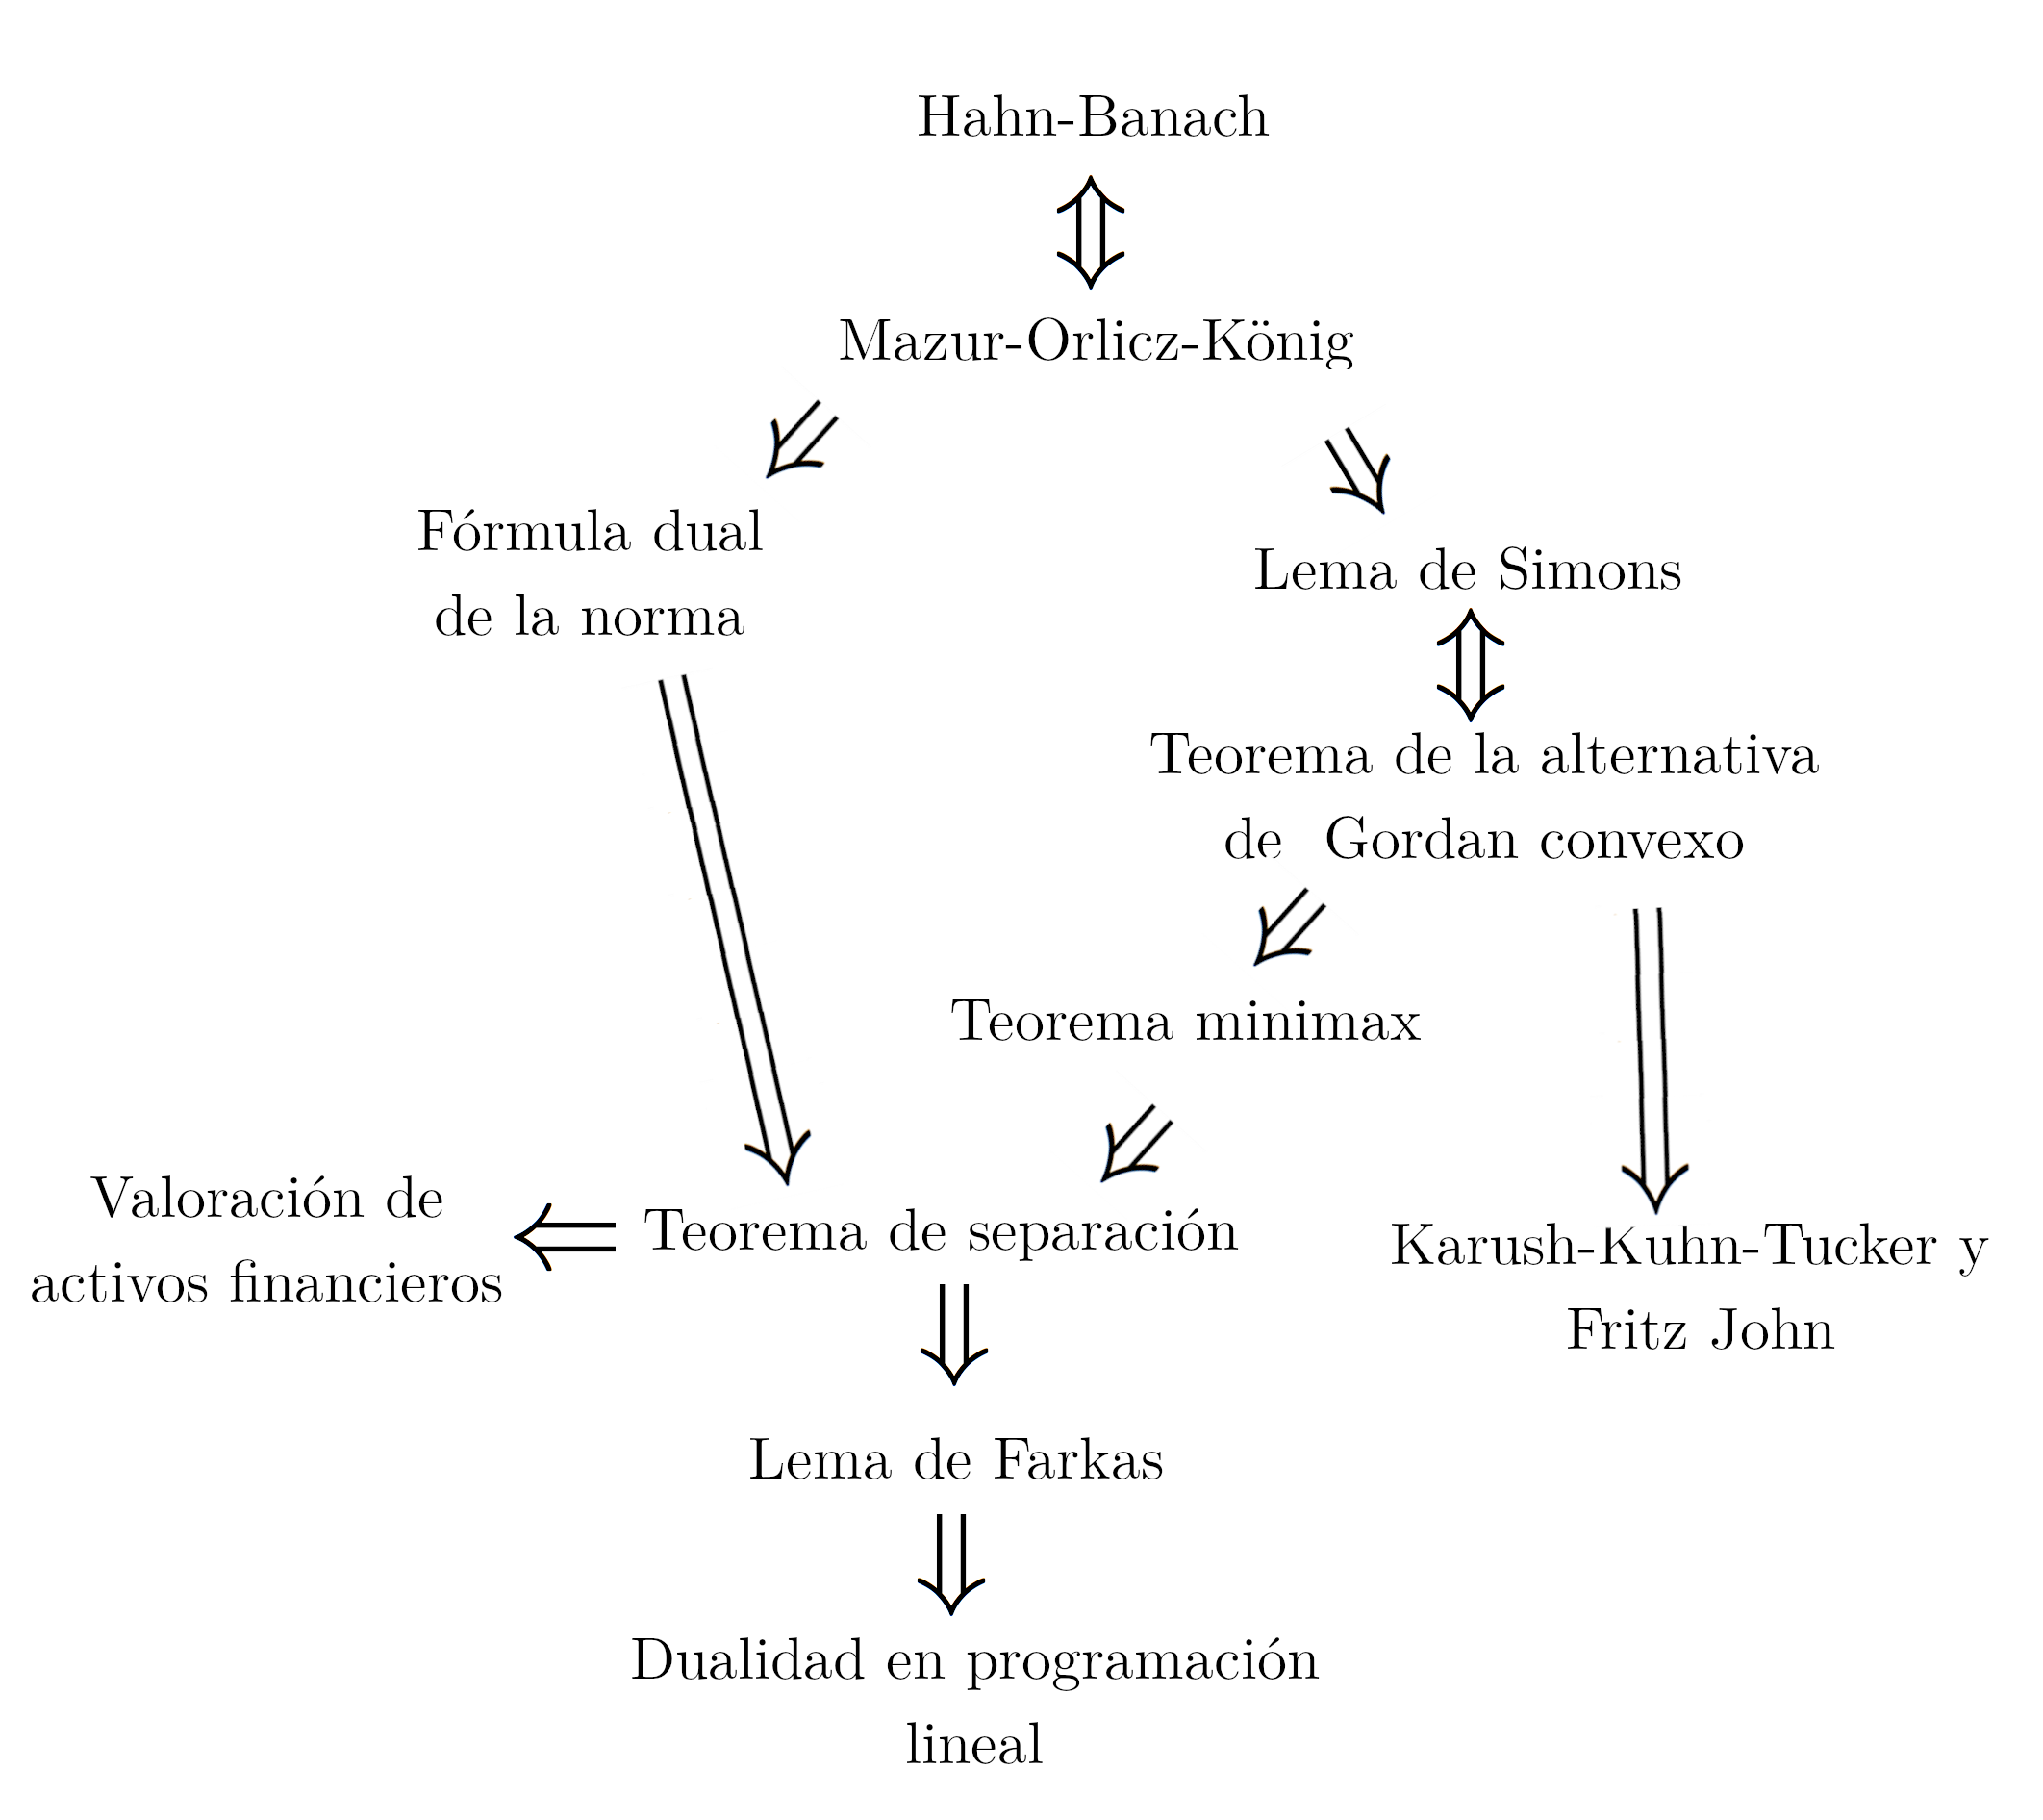
\includegraphics[width=0.9\linewidth]{imagenes/esquema.png}
	\label{fig:aux2}
\end{figure}

Como puede observarse, las técnicas son de carácter convexo y analítico funcional.
\\

\part{Teoremas de la alternativa, optimización convexa y valoración de activos financieros}
\chapter{Teoremas de la alternativa}
Los teoremas de la alternativa constituyen una potente herramienta en optimización. A pesar de tener un claro carácter convexo, se aplican incluso a problemas no convexos, tal y como se comprobará a lo largo de esta memoria. Nuestro punto de partida es el resultado del análisis  convexo, más importante, el teorema de Hahn-Banach. Es más, daremos una versión equivalente debida a H. König, conocida como el teorema de Mazur-Orlicz-König. Como consecuencia, obtendremos el teorema de la alternativa de Gordan, tanto en su versión convexa como una más general. 

\section{Teorema de Mazur-Orlicz-König}
El objetivo principal de esta sección es demostrar una versión equivalente no muy conocida del clásico teorema de Hanh-Banach, el teorema de Mazur-Orlicz-König. Iremos de una versión básica y algebraica del teorema de Hahn-Banach al teorema de Mazur-Orlicz-König siguiendo como aparece en el texto de S. Simons \cite{Simons2008}. \\
	
En primer lugar vamos a recordar la definición de funcional sublineal sobre un espacio vectorial \vecSpace . Notar que todos los espacios vectoriales que vamos a usar son reales. Del mismo modo, los espacios y conjuntos que usaremos asumiremos que son no vacíos.
	
\begin{definicion}
Sea \vecSpace un espacio vectorial. Decimos que el $P:\vecSpace \rightarrow \RR$ es sublineal si cumple las siguientes condiciones:
	\begin{itemize}
		\item $ P $ es subaditiva: $x_1, x_2 \in \vecSpace \Longrightarrow P(x_1 + x_2) \leq P(x_1) + P(x_2) $.
		\item $ P $ es positivamente homogénea: $x_1 \in \vecSpace $ y $ \lambda > 0 \Longrightarrow P(\lambda x) = \lambda P(x) $.
	\end{itemize}
\end{definicion}

Como consecuencia, podemos afirmar que $ P(0) = 0 $. En efecto:
\[
P(0) = P(2\times0) = 2\times P(0) \Longrightarrow P(0) = 0.
\]

Por ejemplo, toda norma o incluso toda seminorma sobre \vecSpace es un funcional sublineal. Así, dados $ a,b \in \RR $ con $ a <b $ tenemos que $ P:H^{1} (a,b) \longrightarrow \RR$ definida como \[ P(x) = \norm{x'}_{L^2(a,b)} \] es una seminorma y por ello sublineal. También, si $ \vecSpace = \RR $ y definimos la parte positiva \[ P(x) = [x]^{+} = \max \{0,x\}, \forall x \in \RR \] obtenemos un funcional sublineal sobre $\RR$. \\
	
El lema que exponemos a continuación, y que generalizaremos posteriormente en el lema \ref{lema2}, nos servirá para demostrar el teorema de Hanh-Banach. 
	
\bigskip
	\begin{lemaBox}\label{lema1}
		Sea\vecSpace un espacio vectorial y $P:\vecSpace \rightarrow \RR$ un funcional sublineal. Fijamos un elemento $ y \in \vecSpace $ y para todo $ x \in \vecSpace $ tomamos  
		\begin{center}
			$ P_y(x) := \displaystyle\inf_{\lambda > 0} \left[P(x+\lambda y) - \lambda P(y)\right] $
		\end{center}
		
		Entonces, $ P_y(\vecSpace) \subset \RR$, $ P_y:\vecSpace \longrightarrow \RR $ es sublineal, $ P_y \leq P $ y además $ P_y (-y) \leq  -P(y)$.
	\end{lemaBox} 
	\begin{proof}
		Fijamos $ y \in V $. Sea $ x \in V $ y $ \lambda > 0$. Como P es sublineal tenemos: 
		\begin{center}
			$ \lambda P(y) = P(\lambda y) =P(\lambda y +x-x) \leq P(x+\lambda y)+ P(-x)$.
		\end{center}
		Por lo tanto, se obtiene que $ P(x+\lambda y) - \lambda P(y) \geq -P(-x) $.  Tomando el ínfimo sobre $ \lambda >0 $ llegamos a $ P_{y}(x)\geq -P(-x) > -\infty$. Por consiguiente, $ P_y(\vecSpace) \subset \RR$, esto es $ P_y:\vecSpace \longrightarrow \RR $. \\
		
		Probaremos ahora que $ P_y $ es sublineal. Empezamos viendo la subaditividad. Tomamos $ x_1, x_2 \in V $ y sean $ \lambda_1, \lambda_2 > 0$ arbitrarios. Entonces, la definición de $ P_y $ da 
		\begin{equation*}
		\begin{split}
		( P(x_1 + \lambda_1 y) - \lambda_1 P(y) ) &+ ( P(x_2 + \lambda_2 y) - \lambda_2 P(y) ) \\
		& \geq ( P(x_1 + x_2 + (\lambda_1+\lambda_2)y)) - (\lambda_1+\lambda_2) P(y) \\
		&\geq P_y (x_1 + x_2 ).
		\end{split}
		\end{equation*}
		Tomando ínfimos sobre $ \lambda_1 $ y $ \lambda_2 $, $  P_y (x_1)  + P_y (x_2 ) \geq P_y (x_1 + x_2 ) $. Así, $ P_y $ es subaditiva. Para comprobar que es positivamente homogénea tomamos $ x \in V $ y $ \mu > 0 $. Entonces:
		\begin{equation*}
		\begin{split}
		P_y (\mu x) &= \inf_{\lambda > 0} \left[P(\mu x+\lambda y) - \lambda P(y)\right] \\
		&= \mu \inf_{\lambda > 0} \left[P(x+ (\lambda / \mu) y) - (\lambda / \mu) P(y)\right] \\
		&= \mu \inf_{\upsilon > 0} \left[P(x+ \upsilon y) - \upsilon  P(y)\right] \\
		&= \mu P_y (x).
		\end{split}
		\end{equation*}	
		Obtenemos que $ P_y $ es positivamente homogénea y como consecuencia sublineal. \\
		
		Para demostrar que $ P_y \leq P $, sea $ x \in V $ y tomando $ \lambda = 1 $ en la definición de $ P_y $,
		\[ P_y(x) \leq P(x+y) - P(y) \leq P(x)+ P(y) - P(y) = P(x) \]
		Como $ x \in \vecSpace $ es arbitrario, entonces $ P_y \leq P $. Finalmente, razonando de manera similar,
		\[P_y(-y) \leq P(-y+y) - P(y) = -P(y).  \]
		
	\end{proof}
\bigskip
El teorema de Hahn-Banach que hemos mencionado antes (básico y algebraico) se enuncia en estos términos:

\bigskip
	\begin{teoremaBox}[Hanh-Banach]\label{H-B}
		Sea V un espacio vectorial y $P:V \rightarrow \RR$ un funcional sublineal. Entonces existe un funcional lineal $ L:\vecSpace \longrightarrow \RR $ tal que $ L \leq P $.
	\end{teoremaBox}
\begin{figure}[h!]
	%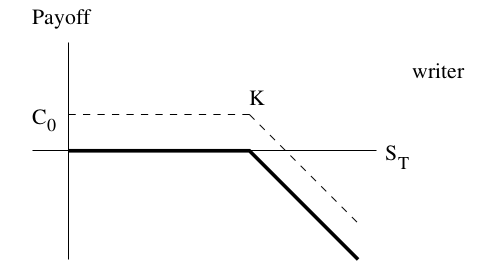
\includegraphics[width=1\linewidth]{Writer_call}
	\centering
	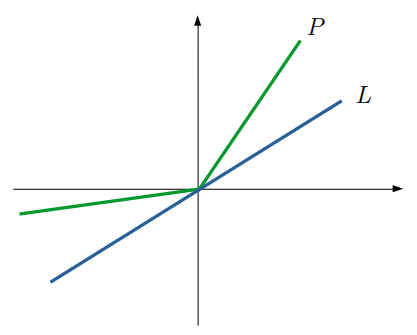
\includegraphics[width=0.6\linewidth]{H-B}
	\caption{Teorema de Hahn-Banach.}
\end{figure}

	\begin{proof}
		Sea $ \text{SUB} = \lbrace Q:\vecSpace \longrightarrow \RR : Q \leq P \rbrace$, es decir, el conjunto de funcionales sublineales sobre \vecSpace que minoren a $ P $. Nuestro propósito es emplear el lema de Zorn con objeto de probar que tiene un elemento minial y tal elemento será el funcional $ L $ que buscamos. Para ello, dados $ T_1 ,T_2 \in \text{SUB} $ consideramos la relación de orden usual, es decir:
		\begin{center}
			$ T_1 \leq T_2 \Longleftrightarrow T_1 (x) \leq T_2 (x) \quad \forall x \in \vecSpace $.
		\end{center}
		Primero probaremos que todo subconjunto $ \mathcal{T} $ totalmente ordenado de $SUB $ tiene una cota inferior en  SUB. Definimos $ Q(x):=\inf \{ T(x): T \in \mathcal{T} \} $ y queremos ver que $ Q(x) \in \RR $. Si $ x \in \vecSpace $ y $ T \in \mathcal{T} $, como T es subaditiva obtenemos la siguiente relación:
		\[ 0 = T(0) = T(x-x) \leq T(x) + T(-x) \Longrightarrow T(x) \geq -T(-x) \quad (1)\]  
		Por otro lado:
		\[ T \in \mathcal{Q} \Longrightarrow T(x) \leq P(x) \Longrightarrow -T(x) \geq -P(x) \quad (2)\] 
		Usando (1), (2) y tomando ínfimo sobre $  T $  llegamos a $ Q(x) \geq -P(x) \geq - \infty $. Por lo tanto $ Q:V \rightarrow \RR$. \\
		
		Ahora probaremos que $ Q $ es subaditiva. Para ello, tomamos $ x_1, x_2\in \vecSpace $. Sean $ T_1 , T_2 \in \mathcal{T} $ arbitrarios. Si $ T_1 \geq T_2 $ (el caso de $ T_2 \geq T_1 $ es análogo.):
		
		\begin{center}
			$ T_1 (x_1)+  T_2 (x_2) \geq T_2(x_1)+  T_2 (x_2) \geq T_2(x_1 +x_2) \geq Q(x_1 + x_2).$
		\end{center}
		Concluimos (en ambos casos) que $ T_1 (x_1)+  T_2 (x_2) \geq Q(x_1 + x_2)$. Tomando ínfimo en $ T_1 $ y $ T_2 $ obtenemos que $ Q (x_1)+  Q(x_2) \geq Q(x_1 + x_2)$. Así, $ Q $ es sublineal. Que sea positivamente homogénea es consecuencia de que $ T $ también lo es. Dado $ \mu > 0 $:
		\begin{equation*}
		\begin{split}
		Q(\mu x) &=\inf \{ T(\mu x): T \in \mathcal{T} \} \\ 
		& = \inf \{ \mu T( x): T \in \mathcal{T} \} \\ 
		&= \mu\inf \{ T( x): T \in \mathcal{T} \} \\ 
		&= \mu Q(x). 
		\end{split}
		\end{equation*}
		
		De este modo, Q es sublineal y como es claro que $ Q \leq P \Longrightarrow Q \in \text{SUB} $. Así, es directo que $ Q $ es el elemento minimal de $ \mathcal{T} $ en SUB.\\
		
		El lema de Zorn nos proporciona entonces un elemento minimal de SUB que llamaremos $ L $. Vamos a comprobar que $ L $ es lineal y, por tanto, es el funcional buscado. Tomamos ahora $ y \in \vecSpace $. Con la notación del lema anterior, $ L_y : \vecSpace \longrightarrow \RR $ es sublineal, $ L_y \leq L $ (como consecuencia $ L_y \in \text{SUB} $) y $ L_y (-y) \leq L(-y) $. De hecho, como $ L $ es minimal en SUB, $ L_y = L $ y por ello $ L (-y) \leq L(-y) $. Por otro lado, como L es subaditiva, $ L(-y) \geq -L(y) $. Combinando ambas desigualdades, $ L(-y) = -L(y) $. Tomamos $ x \in \vecSpace $ y $ \lambda < 0 $, usando la igualdad anterior llegamos a:
		\[ \qquad \quad
		L(\lambda x) = L (-(-\lambda)x) = -L(-\lambda x) = -(-\lambda)L(x) = \lambda L(x) \label{1}
		\] 
		obteniendo que $ L $ es homogénea. Si $ x_1, x_2 \in \vecSpace $, la subaditividad de $ L $ nos da $ L(-x_1-x_2) \leq L(-x_1) + L(-x_2) $. Usando la homogeneidad de $ L $:
		\begin{equation*}
		\begin{split} \qquad
		L(x_1+x_2) &= L(-(-x_1-x_2)) = -L(-x_1-x_2) \\ 
		& \geq -L(-x_1)-L(-x_2) = L(x_1) + L (x_2) \geq L(x_1+x_2). 
		\end{split}
		\end{equation*}
		Por ello, $	L(x_1+x_2) = L(x_1) + L (x_2) $ y por la arbitrariedad de $ x_1, x_2 \in \vecSpace $ concluimos que $ L $ es lineal.
		
	\end{proof}
\bigskip

Nos disponemos a probar, a partir de el teorema de Hahn-Banach el de Mzur-Orlicz-König, que supone un refinamiento. Antes, necesitamos un resultado técnico, que constituye una especie de versión global sobre un convexo del lema \ref{lema1}.
	
\bigskip 
	\begin{lemaBox}\label{lema2}
		Sea\vecSpace un espacio vectorial y $P:\vecSpace \rightarrow \RR$ un funcional sublineal. Sea $ D $ un subconjunto convexo de \vecSpace y sea $ \beta := \inf_D P \in \RR $. Para todo $ x \in V $ tomamos  
		\begin{center}
			$ Q(x) := \inf_{d \in D, \lambda > 0} \left[P(x+\lambda d) - \lambda \beta\right] $
		\end{center}
		
		Entonces, $ Q(\vecSpace) \subset \RR $, $ Q:V \rightarrow \RR$ es sublineal, $ Q \leq P $ y además $ \forall d \in D$ se cumple  $-Q(-d) \geq \beta$.
	\end{lemaBox} 
	\begin{proof}
		Si $ x \in \vecSpace,\text{ }d \in D $ y $ \lambda > 0 $, entonces
		\begin{center}
			$ P(x+ \lambda d) - \lambda \beta \geq -P(-x) + \lambda P(d)-\lambda\beta \geq -P(-x) \geq -\infty$.
		\end{center}
		La primera desigualdad se deduce de la linealidad de P ya que:
		\begin{equation*}
		\begin{split}
		\lambda P(d) &= P(\lambda d) \\ 
		&=P(\lambda d +x-x) \\ 
		&\leq P(x+\lambda d)+ P(-x)
		\end{split}
		\end{equation*}
		por lo que $ \lambda P(d)-P(-x) \leq P(x+\lambda d) $. La segunda se debe a que
		\[\beta = \inf_D P \Longrightarrow \lambda P(d) \geq \lambda\beta \Longrightarrow\lambda P(d) - \lambda\beta \geq 0. \]
		Tomando el ínfimo sobre $ d \in D  $ y $ \lambda > 0 $ llegamos a \[ Q(x)\geq -P(-x) > -\infty,\] por lo que $ Q(\vecSpace) \longrightarrow \RR$. Es relativamente fácil probar que $ Q $ es positivamente homogénea por lo que para ver que es sublineal solo queda comprobar la subaditividad. Para ello, tomamos $ x_1, x_2 \in V $. Sean $ d_1, d_2 \in D $ y $ \lambda_1, \lambda_2 > 0$ arbitrarios. Para simplificar la notación llamamos $ x := x_1 + x_2 $, $ \lambda := \lambda_1 + \lambda_2 $ y $ d:= (\lambda_1/\lambda)d_1 + (\lambda_2/\lambda)d_2 $. Notar que $ d \in D $, al ser este convexo. Entonces: 
		\begin{equation*}
		\begin{split}
		( P(x_1 + \lambda_1 d_1) - \lambda_1 \beta ) + ( P(x_2 + \lambda_2 d_2) - \lambda_2 \beta ) &\geq P(x + \lambda_1 d_1 + \lambda_2 d_2) - \lambda \beta\\
		& = P(x +\lambda d) - \lambda \beta\\ 
		& \geq Q(x) = Q(x_1 + x_2).
		\end{split}
		\end{equation*}
		Tomando ínfimo sobre $ d_1, d_2, \lambda_1 $ y $ \lambda_2 $, $  Q(x_1) + Q (x_2 ) \geq Q (x_1 + x_2 ) $. Así, $ Q $ es subaditiva y como consecuencia sublineal. Para concluir, fijamos $ d \in D $. Sea $ x \in \vecSpace $ arbitrario. Entonces, $ \forall \lambda > 0 $, $ Q(x) \leq P(x) + \lambda (P(d) - \beta )$. Tomando $ \lambda \longrightarrow 0 $, $ Q(x) \leq P(x)$ y como consecuencia $ Q \leq P $. Finalmente, sea $ d \in D $ arbitrario y tomando $ \lambda = 1 $:
		\[Q(-d) \leq Q(-d+d) - \beta = -\beta \Longrightarrow  -Q(-d) \geq \beta.  \]
		
	\end{proof}
\bigskip

Ya estamos preparados para probar el teorema de Mazur-Orlicz-König, debido a H. König \cite{König1, König2}. No solo es una versión equivalente del teorema de Hahn-Banach, también de un teorema de Mazur-Orlicz \cite{mo}, aunque es solo una reformulación. 

\bigskip
	
	\begin{teoremaBox}[Mazur-Orlicz-König]\label{M-O}
		Sea\vecSpace un espacio vectorial y $P:\vecSpace \rightarrow \RR$ un funcional sublineal.  Sea $ D $ un subconjunto no vacío y convexo de \vecSpace. Entonces existe un funcional $ L: \vecSpace \longrightarrow \RR $ lineal tal que $ L \leq P $ e $ \inf_D L = \inf_D P $.
	\end{teoremaBox}

Antes de pasar a la demostración, observemos que, aunque es un resultado puramente algebraico, tiene una fuerte interpretación geométrica: el teorema de Hahn-Banach garantiza, dado un funcional sublineal, $ P: \vecSpace \longrightarrow \RR $, la existencia de un funcional lineal $ L:\vecSpace \longrightarrow \RR $ con $ L \leq P $. En la imagen \ref{H-B-varios} mostramos unos ejemplos de funcionales que nos aporta el teorema de Hahn-Banach. \\

\begin{figure}[h!]
	%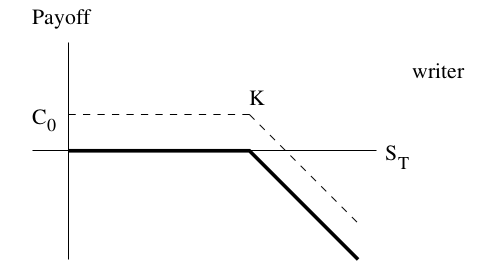
\includegraphics[width=1\linewidth]{Writer_call}
	\centering
	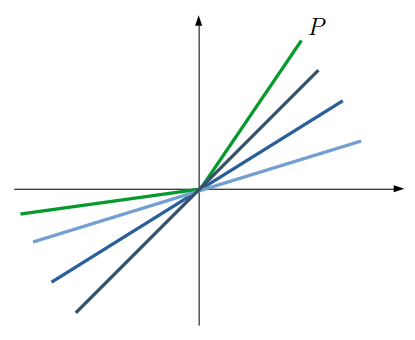
\includegraphics[width=0.6\linewidth]{H-B_2}
	\caption{Ejemplos de funcionales aportados por el teorema de Hahn-Banach.}
	\label{H-B-varios}
\end{figure} 

El teorema de Mazir-Orlicz-König, fijado un subconjunto convexo $ D $ de $ \vecSpace $, nos da solo los funcionales lineales que minoran a $ P $ y que cumplen
\[
\inf_D L = \inf_D P.
\]
En la imagen \ref{M-O-K-fotos} se muestra un ejemplo del teorema.
\begin{figure}[h!]
	%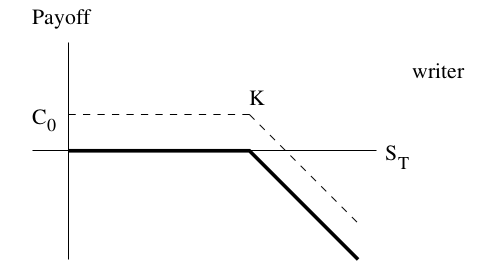
\includegraphics[width=1\linewidth]{Writer_call}
	\centering
	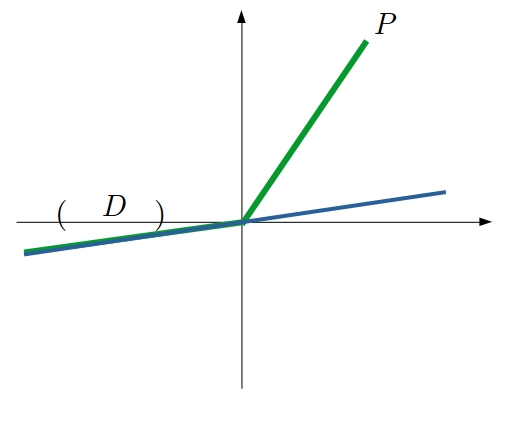
\includegraphics[width=0.6\linewidth]{M-O-K}
	\caption{Teorema de Mazur-Orlicz-König.}
	\label{M-O-K-fotos}
\end{figure} 

	\begin{proof}
		Sea $ \beta := \inf_D P $. En el caso de que $ \beta = -\infty $ por el teorema de Hanh-Banach tenemos que $ \exists L $ sobre \vecSpace tal que es lineal y $ L \leq P$. Así:
		\begin{center}
			$ L \leq P \Longrightarrow inf_D L \leq \inf_D P = -\infty \Longrightarrow inf_D L = \inf_D P.$ 
		\end{center}
		Supongamos entonces que $ \beta \in \RR $. Definimos el funcional auxiliar $ Q $ como en el lema \ref{lema2}. Del teorema de Hanh-Banach obtenemos que existe un funcional lineal $ L $ sobre \vecSpace tal que $ L \leq Q$ (como $ Q \leq P $ tenemos que $ L \leq P $). Sea $ d \in D $, entonces:
		\[
		L(d) = -L(-d) \geq -Q(-d) \geq \beta.
		\]
		Tomando ínfimo sobre $ d \in D $:
		\[
		\inf_D L \geq \beta = \inf_D P.
		\]
		Por otro lado, como $ L \geq P $:
		\[
		\inf_D L \leq\inf_D P.
		\]
		Juntando ambas desigualdades obtenemos $ \inf_D L =\inf_D P $.
	\end{proof}

\bigskip

%%% IGUALDAD
\newcommand{\normSpace}{E}
Antes de probar la eficiencia del teorema de Mazur-Orlicz-König en el siguiente apartado, presentamos una consecuencia bien conocida. En particular, nos será de utilidad posteriormente para el teorema de Separación. Recordemos dados $ \normSpace_1, \normSpace_2 $ dos espacios normados y $ T:\normSpace_1 \longrightarrow \normSpace_2 $ un operador lineal, entonces $ T $ es continuo si, y solo si, verifica la siguiente condición:
\[
\exists \alpha > 0 : \norm{T(x)} \leq \alpha \norm{x} \quad \forall x \in \normSpace_1,
\]
Consideramos el espacio vectorial dado por:
\[
\normSpace^* =  \lbrace T:\normSpace \longrightarrow \RR: T \text{ es lineal y continuo} \rbrace.
\]
conocido como el espacio dual (topológico) de $ E $. Para todo $ T \in \normSpace^* $ definimos su norma como:
\[
\norm{T} = \min \lbrace \alpha > 0:  \abs{T(x)} \leq \alpha \norm{x} \quad \forall x \in \normSpace\rbrace.
\]
De este modo, podemos escribir:
\begin{equation*}\label{desigNorma}
\abs{T(x)} \leq \norm{T} \norm{x}
\end{equation*}
siendo dicha desigualdad óptima. También podemos expresar su norma como el mínimo mayorante de un conjunto mayorado, es decir, el supremo:
\[
\norm{T} = \sup \lbrace \norm{T(x)}/\norm{x} : \forall x \in \normSpace \setminus \{0\}\rbrace.
\]
Para $  x \in \normSpace_1 \setminus \{0\} $ tenemos que $ \abs{T(x)}/\norm{x} = \norm{T(x/\norm{x})}$ y es claro que $ \{ x/\norm{x} : x \in \normSpace_1 \setminus \{0\}\} $ es la esfera unidad de $ \normSpace $ que notamos como $ S_\normSpace $. Si en vez de la esfera consideramos la bola unidad, $ B_\normSpace $ el supremo no varía. Efectivamente, si $ x \in B_\normSpace  $ se tiene que $ x = \norm{x}u $ con $ u \in  S_\normSpace$, y por ello $ \abs{T(x)} = \norm{x}\norm{T(u)} \leq \abs{T(u)} $ ya que $ \norm{x} \leq 1 $. De este modo, también tenemos que:
\begin{equation*}\label{normSup}
\norm{T} =\sup_{x \in B_\normSpace} \abs{T(x)}.
\end{equation*}

En este momento, estamos en disposición de enunciar y demostrar la igualdad que deseamos:

\bigskip
\begin{corolarioBox}\label{iguSupNor}
	Dado un espacio normado $ \normSpace $ y $ x \in \normSpace $, entonces se cumple que:
	\begin{equation}\label{iguNorm}
	\sup_{x^* \in B_{\normSpace ^ *}} x^*(x) = \norm{x}.
	\end{equation}
\end{corolarioBox}
\begin{proof}
	Sea $ x_0 \in E$ y sea $ D := \{x_0\} $. Consideramos el funcional 
	\begin{equation*}
	\begin{split}
	P:\normSpace \longrightarrow &\RR \\
	x \longmapsto &\norm{x}.
	\end{split}
	\end{equation*} 
	Es claro que $ P $ es sublineal y que $ D $ es convexo. Podemos aplicar el Teorema de Mazur-Orlicz-König, teorema \ref{M-O}, y obtenemos que existe un funcional $ L:\normSpace \longrightarrow \RR $ lineal tal que $ L \leq P $ e $ \inf_D L = \inf_D P $. Como $ L \leq P $, entonces 
	\begin{equation*}
	\norm{L(x)} \leq \norm{P(x)} = \norm{x} \quad \forall x \in \normSpace.
	\end{equation*}
	Concluimos que $ L $ es continua. Además, como tenemos que $ L \in \normSpace ^* $, llamamos $ L = x^* $ y llegamos a que $ \norm{L} = \norm{x^*}  \leq 1$, es decir, $ x^* \in  B_{\normSpace ^ *} $.  Por su parte, como  $ \inf_D L = \inf_D x^* = \inf_D P $ y $ D = \{x_0\} $ entonces, $ x^*(x_0) = \norm{x_0} $. De este modo, llegamos a que existe $ x^* \in B_{\normSpace^*} $ tal que $ x^*(x_0) = \norm{x_0} $. Si tomamos cualquier elemento $ y^* \in B_{\normSpace^*}  $, entonces \[ \norm{y^*(x_0)} \leq \norm{y^*} \norm{x_0} \leq \norm{x_0} \] y podemos asegurar que:
	\[
	\sup_{x^* \in B_{\normSpace ^ *}} x^*(x_0) = \norm{x_0}.
	\] 
	Como $ x_0 \in \normSpace $ es arbitrario, la desigualdad enunciada queda probada.
\end{proof}
\bigskip

\section{Teorema de la alternativa de Gordan. Reformulaciones.}
\newcommand{\ttt}{\textbf{\emph{t}}}
\newcommand{\sss}{\textbf{\emph{s}}}
\newcommand{\xx}{\textbf{\emph{x}}}
\newcommand{\yy}{\textbf{\emph{y}}}
\newcommand{\vv}{\textbf{\emph{v}}}
\newcommand{\ww}{\textbf{\emph{w}}}
\newcommand{\zz}{\textbf{\emph{z}}}

Una vez que disponemos de la herramienta fundamental, el teorema de Mazur-Orlicz-König, nos disponemos a dar una versión convexa del teorema de la alternativa de Gordan. Antes de ello, y haciendo uso de este teorema tipo Hahn-Banach, probaremos el lema de Simons, sobre cierta condición de optimalidad para funciones convexas. \\

Antes de comenzar, necesitamos hacer la siguiente definición. Para agilizar la lectura, cuando indicamos $ N\in \NN $ estamos suponiendo que $ N \geq 1 $. También, para $ N \in \NN $, notaremos con caracteres en negrita a los elementos de $ \RR^N $, por ejemplo, $  \ttt = (t_1,...,t_N)\in \RR^N$. 

\begin{definicion}
	Dado $ N \in \NN $ llamamos símplex unitario de $ \RR^N $ al conjunto de $ \RR^N $ definido como:
	\begin{equation*}
	\Delta_N := \left\lbrace \ttt \in \RR^N: \sum_{i=1}^{N}{t_i} = 1, \hspace{0.5em} t_1,...,t_N \geq 0 \right\rbrace .
	\end{equation*}
\end{definicion}

Recordamos ahora la noción de envolvente convexa de un subconjunto cualquiera $ X $ de un espacio vectorial $ \vecSpace $, que notamos como $ \mathrm{co}(X) $ y que se define como la intersección de todos los conjuntos convexos que contienen a $ X $. Nótese que $ \Delta_N = \mathrm{co}\{e_1,...e_N\} $. \\

Antes de continuar veamos que $ \Delta_N $ es convexo y compacto:

\begin{itemize}
	\item  Convexo: tenemos que comprobar que dados $ \ttt, \sss \in \Delta_N \text{ y } \lambda \in \lbrack 0,1 \rbrack $ entonces $ \lambda\ttt + (1-\lambda)\sss \in \Delta_N $. En efecto, las coordenadas $ \lambda t_i + (1-\lambda)s_i $ verifican:
	\begin{itemize}
		\item [i) ] $ \lambda t_i + (1-\lambda)s_i \geq 0 $ para todo $ i = 1,..., N $, ya que $ t_i, s_i \geq 0 $ y $ 0 \leq \lambda \leq 1 $.
		\item [ii) ] 
		\begin{equation*}
		\begin{split}
		\sum_{i=1}^{N} (\lambda t_i + (1-\lambda)s_i) &=   \lambda \sum_{i=1}^{N} t_i + (1-\lambda)\sum_{i=1}^{N} s_i \\
		&= \lambda + (1 - \lambda) \\ &= 1,
		\end{split}
		\end{equation*}ya que $ \sum_{i=1}^{N} t_i = \sum_{i=1}^{N} s_i = 1  $.
	\end{itemize}
	
	Por lo tanto, $ \lambda\ttt + (1-\lambda)\sss \in \Delta_N \text{ para todo }\lambda \in \lbrack 0,1 \rbrack $.
	
	\item Compacto: al encontrarnos en $ \RR^N $ y aplicando el conocido Teorema de Heine-Borel basta y sobra ver que $ \Delta_N $ es cerrado y acotado. Pero claramente es acotado por lo que nos centraremos en probar que es cerrado. Sea $ \lbrace \ttt_n \rbrace_{ n \in \NN} $ una sucesión de $ \Delta_N $ y sea $ \ttt_0 \in \RR^N $ tal que $ \lbrace \ttt_n \rbrace_{ n \in \NN} \longrightarrow \ttt_0 $. Tenemos que comprobar que $ \ttt_0 \in \Delta_N $. 
	\begin{itemize}
		\item[i) ] Como todas las coordenadas de cada $ \ttt_n $ para $ n \in \NN $ son no negativas las de $ \ttt_0 $ también lo son.
		\item[ii) ] La función $ f: \RR^N \longrightarrow \RR $ definida como $ f(\ttt) =  \sum_{i=1}^{N} t_i $ es continua. Claramente $ f(\ttt) = 1 $ para todo $ \ttt \in \Delta_N $ y por ello $ \lbrace f(\ttt_n) \rbrace_{ n \in \NN} \longrightarrow 1$. Por continuidad de $ f $ y unicidad de límite tenemos que $ f(\ttt_0) = 1 $ pero eso equivale a que la suma de sus componentes vale 1.
	\end{itemize} 
	
	Así, hemos demostrado que $ \ttt_0 \in \Delta_N $ y por lo tanto $ \Delta_N $ es compacto. 
\end{itemize}


\paragraph{}Antes de continuar, notamos que el espacio vectorial de todas las aplicaciones lineales de $ \RR^N $ a $ \RR $, con $ N \in \NN $, se puede identificar con $ \RR^N $. Esto se debe a que si $ L:\RR^N \longrightarrow \RR $ es lineal, entonces es de la forma $ L(\xx) = a_1x_1 + \cdots + a_Nx_N $, que se corresponde con $ \textbf{\emph{a}} = (a_1,\dots,a_N) \in \RR^N $. Del mismo modo, dado el vector tenemos la aplicación lineal asociada. En definitiva, el espacio dual de 
$ \RR^N $ se identifica con $ \RR^N $ .
\paragraph{} También presentamos el producto escalar usual en $ \RR^N $ que definimos como:
\[
\begin{split}
\langle \cdot, \cdot \rangle : \RR^N \times \RR^N \longrightarrow &\RR \\
(\xx, \yy) \longmapsto &\langle \xx, \yy \rangle = \sum_{i=0}^{N}x_iy_i.
\end{split}
\]

Antes de enunciar el lema de Simons, hacemos otra identificación, esta vez, correspondiente a un símplex unitario:
\bigskip
\begin{lemaBox}\label{lema2.1}
	Sea $ N \in \NN $ y $ S: \RR^N \longrightarrow \RR $ definida por: \[ S(\xx):=\max\{x_1,...,x_N\}.\] Entonces, $ S $ es sublineal. Además, si $ L:\RR^N \longrightarrow \RR $ es un funcional lineal tal que $ L \leq S $ entonces $ L $ es de la forma \[ L(\xx) = t_1 x_1 + ... + t_N x_N \] con $ (t_1,...,t_N) \in \Delta_N$. De hecho, el recíproco también es cierto, es decir, si $ L = \ttt = (t_1,...,t_N) \in \Delta_N $ entonces $ L \leq S $.
	
	%%%%%% NOTA %%%%%%%%
	%% Las aplicaciones lineales coninciden con el dual del espacio. Es decir, podemos identificar la aplicación con sus coeficientes obeniendo de ese modo un punto del espacio.
	
\end{lemaBox}
\begin{proof}
	Claramente, $ S $ es positivamente homogénea. También es sub\-aditiva ya que dados $ x,y \in \vecSpace $ : 
	\begin{equation*}
	\begin{split}
	S(\xx+\yy) &= \max \{x_1 + y_1, ..., x_N +y_N \}\\ 
	&\leq \max\{x_1, ..., x_N\} + \max \{y_1, ...,y_N\} = S(\xx) + S(\yy).
	\end{split}
	\end{equation*}
	
	Por ello, $ S $ es sublineal. Para terminar veamos que  \[\left\lbrace L:\RR^N \longrightarrow \RR : L \text{ lineal y }L\leq S \right\rbrace  =  \Delta_N \]
	a través de la correspondencia mostrada anteriormente entre $ \RR^N $ y su dual.
	
	\begin{itemize}
		\item[$ \supseteq $ )] Sea $ \mathbf{t} \in \Delta_N$, definimos $ L:\RR^N \longrightarrow \RR $ como $ L(\xx):= \langle \mathbf{t},\xx \rangle $. Es evidente que $ L $ es lineal en $ \xx $ al ser el producto escalar bilineal. Dado $ \xx \in \RR^N $,
		\begin{equation*}
		L(\xx) = \sum_{i=1}^{N}{t_i x_i} \leq \sum_{i=1}^{N}{t_i S(\xx)} = S(\xx)\sum_{i=1}^{N}{t_i} = S(\xx),
		\end{equation*}
		donde la primera desigualdad se debe a que $ x_i \leq S(\xx)$ para todo $ x_i$ con $ i=1,...,N $ y a que $ t_i \geq 0 $ ya que $ \mathbf{t} \in \Delta_N$. Esto también justifica la última igualdad ya que $ \sum_{i=1}^{N}{t_i} = 1 $.
		
		\item[$ \subseteq $ )] Sea $ L = \ttt = (t_1,...,t_N) \in \RR^N $ lineal tal que para todo $ \xx \in \RR^N $ cumple que $ \sum_{i=1}^{N}{t_i x_i} \leq S(\xx)$. Así, si tomamos $ e_i \in \RR^N $ donde $ e_i $ representa el i-ésimo elemento de la base usual de $ \RR^N $ con $ i=1,...,N $, entonces 		
		\begin{equation*}
		L(-e_i) = -t_i \leq 0 \Longrightarrow t_i \geq 0 \quad \forall i=1,...,N.
		\end{equation*}
		Si ahora llamamos $ e = \sum_{i=1}^{N}{e_i} $, obtenemos:
		\begin{equation*}
		\begin{rcases*}
		L(e) = \sum_{i=1}^{N}{t_i} \leq \max \{1, ...,1\} = 1 \\
		L(-e) = -\sum_{i=1}^{N}{t_i} \leq \max \{-1, ...,-1\} = -1
		\end{rcases*} \Longrightarrow \sum_{i=1}^{N}{t_i} = 1.
		\end{equation*}
		Concluimos entonces que $ L = \ttt = (t_1,...,t_N) \in \Delta_N $.
	\end{itemize}
	
\end{proof}
\bigskip

Enunciamos ahora el lema de Simons \cite{Simons2008}. Tal y como se ha mencionado antes, se trata de un resultado sobre funciones convexas y cierta condición de optimalidad: dos funciones distintas poseen el mismo ínfimo en un convexo. Esto sugiere el uso del teorema de Mazur-Orlicz-König.
\bigskip
\begin{lemaBox}[Simons]\label{Simons}
	Sea $ C $ un subconjunto convexo de un espacio vectorial y $ N \in \NN $. Dadas $  $ $ f_1, \dots, f_N : C \longrightarrow \RR $, funciones convexas, entones existe $ \ttt \in \Delta_N $ que cumple
	\[
	\inf_{c \in C}\left[ \max_{i=1\dots,N } f_i(c)\right] = \inf_{c \in C} \left[ \sum_{i=1}^{N} t_i f_i(c) \right].
	\] 
\end{lemaBox}
\begin{proof}
	Sea  $ \vecSpace = \RR^N $. Definimos $S:\vecSpace \longrightarrow \RR $ como \[ S(x_1, ..., x_N) := \max \{x_1, ..., x_N\}. \] Por el lema \ref{lema2.1}, $ S $ es sublineal. Tomamos el subconjunto:
	\[ 
	D = \{ (x_1, ..., x_N)\in V: \exists c \in C \quad \text{ tal que } \quad \forall i = 1,...N,\quad f_i(c) \leq x_i \}.
	\]
	Comprobemos en primer lugar que $ D $ es un subconjunto convexo de $ \vecSpace $. Sean $ x, y \in D $, por ello, existen $ c_x, c_y \in C $ tales que $ f_i (c_x) \leq x_i  $ y $ f_i (c_y) \leq y_i \quad \forall i=1,...,N $. Dado $ \lambda \in [0,1] $, llamamos $ c := (1-\lambda)c_x + \lambda c_y $ que pertenece a $ C $ por ser este convexo. Veamos que $ c $ es el elemento necesario de $ C $ para que cualquier combinación convexa de $ x $ e $ y $ esté en $ D $. Así, para todo $ i =1,...,N  $:	
	\[
	f_i(c) = f_i((1-\lambda)c_x + \lambda c_y) \leq (1-\lambda)f(c_x) + \lambda f(c_y) \leq (1-\lambda)x_i + \lambda y_i ,
	\]
	donde la primera desigualdad se debe a que las $ f_i $ son convexas y la segunda a que $ x,y \in D $. Por ello, $ (1-\lambda)x_i + \lambda y_i \in D , \quad \forall \lambda \in [0,1] $ por lo que $ D $ es convexo. Aplicando el Teorema de Mazur-Orlizc-König, existe $ L $ funcional lineal en $ \vecSpace $ tal que $ L \leq S $ e $ \inf_D L = \inf_D S $. \\
	
	Nuevamente, por el lema \ref{lema2.1} tenemos que $ L = \ttt \in \Delta_N$. Finalmente:
	\[
	\inf_D L =\inf_{c \in C} \left[ \sum_{i=1}^{N} t_i f_i(c) \right]
	\]
	e
	\[
	\inf_D S = \inf_{c \in C}\left[ \max_{i=1\dots,N } f_i(c)\right]
	\]
	por lo que 
	\[ \inf_{c \in C}\left[ \max_{i=1\dots,N } f_i(c)\right] = \inf_{c \in C} \left[ \sum_{i=1}^{N} t_i f_i(c) \right]. \] 
\end{proof}
\bigskip
Enuciamos ahora el Teorema de la Alternativa de Gordan en su versión clásica.
\bigskip
\begin{teoremaBox}[Teorema de la alternativa de Gordan]\label{GordanClasic}
	Dados $N, M \in \NN   $, sean $ \{\xx_1,...\xx_N\}$ con $ \xx_i \in \RR^M \text{ para } i=1,...,N$. Entonces una, y solo una, de la siguientes afirmaciones se cumple:
	
	\begin{itemize}
		\item[i*)] $ \exists \mathbf{t} \in \Delta_N $ tal que  $  0 = \displaystyle \sum_{i=1}^{N}{t_i \xx_i}$.
		\item[ii*)] $ \exists \yy \in \RR^M $ tal que cumple $ \displaystyle \max_{i=1,...,N} \langle \yy, \xx_i \rangle < 0 $.
	\end{itemize}
\end{teoremaBox}
\bigskip
Omitimos esta demostración ya que a continuación mostramos la versión convexa del mismo y será la que probaremos. Después veremos que la versión convexa  implica la clásica por lo que quedará probada. Antes de continuar, destacar que la interpretación geométrica de este resultado se observa en la imágen \ref{fig:gordan-clasic}.

\begin{figure}[h!]
	\begin{minipage}{0.5\textwidth}
		\centering
		%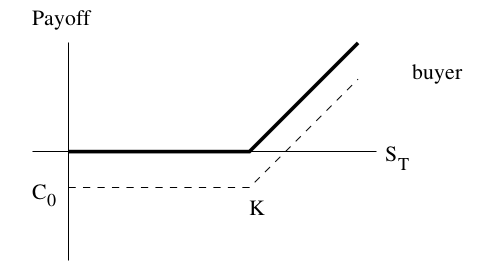
\includegraphics[width=1\linewidth]{Buyer_call} 
		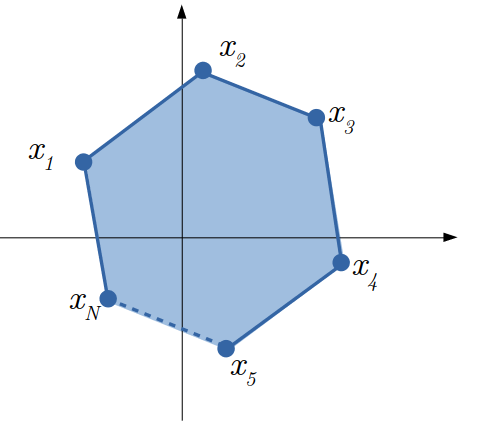
\includegraphics[width=1\linewidth]{Gordan-i*} 
		%\caption{Alternativa $ i*) $.}
		%\label{fig:gordan-i*}
	\end{minipage}
	\begin{minipage}{0.5\textwidth}
		%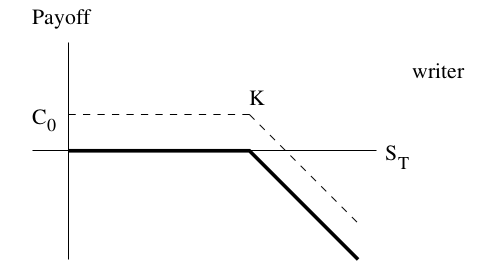
\includegraphics[width=1\linewidth]{Writer_call}
		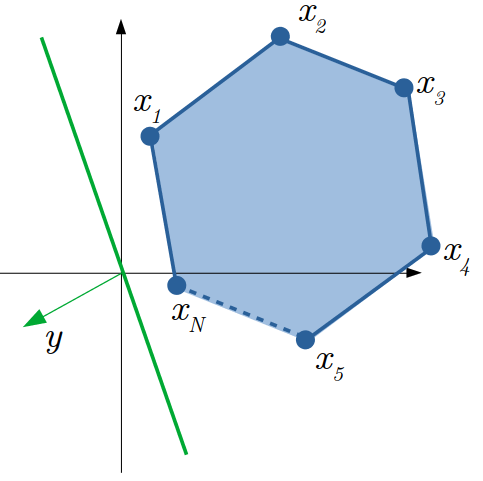
\includegraphics[width=1\linewidth]{Gordan-ii*}
		%\caption{Alternativa $ ii*) $.}
		%\label{fig:gordan-ii*}
	\end{minipage}
	\caption{A la izquierda alternativa $ i*) $ y a la derecha la alternativa $ ii*) $.}
	\label{fig:gordan-clasic}
\end{figure}

\bigskip
\begin{teoremaBox}[Teorema de la Alternativa de Gordan-versión convexa]\label{Gordan}
	Sean $ C $ un subconjunto convexo de un espacio vectorial, $ N \in \NN $ y  $ f_1,...,f_N : C \longrightarrow \RR $ funciones convexas. Entonces una, y solo una, de la siguientes afirmaciones se cumple:
	\begin{itemize}
		\item[i)] $ \exists \mathbf{t} \in \Delta_N $ tal que $ 0 \leq \displaystyle \inf_{c\in C}  \sum_{i=1}^{N}{t_i f_i (c)}$.
		\item[ii)] $ \exists c \in C $ que cumple $\displaystyle \max_{i=1\dots,N } f_i(c) < 0 $.
	\end{itemize}
\end{teoremaBox}
\begin{proof}
	Veamos que las alternativas $ i)$ y $ ii) $ son excluyentes y exhaustivas. Para ello, veamos que $ \neg i) \Longleftrightarrow ii) $. Suponemos inicialmente que $  \inf_{ c\in C}\left[\max_{i=1\dots,N } f_i(c) \right] \in \RR $.
	
	\begin{itemize}
		\item [$ \Leftarrow $)] Si existe $ c_0 \in C $ tal que $ \max_{i=1\dots,N } f_i(c) < 0 $, entonces, dado $ \ttt \in \Delta_N $,
		\[
		\inf_{ c \in C} \sum_{i=0}^{N}t_i f_i(c) \leq \sum_{i=0}^{N}t_i f_i(c_0) < 0
		\]
		donde la última desigualdad se debe a que $ \ttt \in \Delta_N $. Hemos probado entonces $ \neg i) $.
		\item[$ \Rightarrow $)] 	Si aplicamos el lema de Simons, lema \ref{Simons}, a las funciones $ f_1,...,f_N $ obtenemos:
		
		\begin{equation*}
		\exists t \in \Delta_N \text{ : } \inf_{ c\in C}\left[\max_{i=1\dots,N } f_i(c) \right] = \inf_{c \in C} \sum_{i=1}^{N}t_i f_i (c).
		\end{equation*}
		Entonces, de $ \neg i) $ sabemos que, para este $ \ttt \in \Delta_N $ (como para cualquier otro)
		\[
		\inf_{ c \in C} \sum_{i=0}^{N}t_i f_i(c) < 0
		\]
		luego
		\[
		\inf_{ c\in C}\left[\max_{i=1\dots,N } f_i(c) \right] < 0,
		\]
		como queríamos demostrar.
		
	\end{itemize}
	
	Para finalizar, si $  \inf_{ c\in C}\left[\max_{i=1\dots,N } f_i(c) \right] =-\infty $ es claro que estamos en el caso $ ii) $ y se prueba como en el caso de que dicho ínfimo sea un valor real.
\end{proof}
\bigskip
Destacamos las siguientes observaciones:
\bigskip
\begin{observacion}
	Esta versión convexa del teorema implica la versión clásica del mismo.
\end{observacion}

Para ello, basta aplicar la versión convexa del teorema a $ C := \RR^M $ y a las funciones $ f_1,...,f_N : C \longrightarrow \RR $ definidas por \[ f_i(c):=\langle c, \xx_i \rangle , \forall i=1,...,N.\] Notar que las funciones $ f_1,...,f_N $ son lineales por la izquierda y como consecuencia son convexas. En este caso, la alternativa $ ii) $ implica $ ii*) $ ya que:

\begin{equation*}
\exists c \in C = \RR^M \text{ : } \max_{i=1,...,N} {\langle c,x_i \rangle}  =  \max_{i=1,...,N}f_i (c) < 0 .
\end{equation*}
Por su parte, la alternativa $ i) $ nos da:
\begin{equation*}
\exists \mathbf{t} \in \Delta_N \text{ : } 0 \leq \inf_{c \in \RR^M}  \sum_{i=1}^{N}{t_i f_i(c) } = \inf_{c \in \RR^M} \sum_{i=1}^{N}{t_i\langle c, \xx_i \rangle} = \inf_{c \in \RR^M} \langle c, \sum_{i=1}^{N}{t_i 	\xx_i} \rangle. 
\end{equation*}
Hemos obtenido por ello que  $0  \leq \inf_{c \in \RR^M} \langle c, \sum_{i=1}^{N}{t_i \xx_i} \rangle  $ lo que significa que $ 0 \leq \langle c, \sum_{i=1}^{N}{t_i \xx_i} \rangle  $ para todo $ c \in \RR^M $. Usando la bilinealidad del producto escalar:
\[
0 \leq \langle -c, \sum_{i=1}^{N}{t_i \xx_i} \rangle \Longleftrightarrow 	0 \leq -\langle c, \sum_{i=1}^{N}{t_i \xx_i} \rangle 
\Longleftrightarrow  \langle c, \sum_{i=1}^{N}{t_i \xx_i}\rangle \leq 0, \quad \forall c \in \RR^M.
\]
Juntando ambas desigualdades obtenemos que $ 0 =  \langle c, \sum_{i=1}^{N}{t_i \xx_i}\rangle, \quad \forall c \in \RR^M $. Como la igualdad anterior se cumple para todo elemento de $ \RR^M $ entonces podemos deducir que $ \sum_{i=1}^{N}{t_i \xx_i} = 0 $	ya que $ \sum_{i=1}^{N}{t_i \xx_i} \in (\RR^M)^{\perp} = \{0\} $. Así pues, tenemos que $ i) $ equivale a $ i*) $. \hspace{5.7cm}\qedsymbol 

\bigskip
\begin{observacion}
	El lema de Simons (lema \ref{Simons}) y el teorema convexo de la Alternativa de Gordan (teorema \ref{Gordan}) son equivalentes.
\end{observacion}

\paragraph{} Ya hemos visto que el Lema de Simons implica el Teorema de la Alternativa de Gordan. Veamos que el recíproco también es cierto.  \\

Llamamos $ \alpha := \inf_{ c\in C}\left[\max_{i=1\dots,N } \{f_i(c)\} \right] $. Si $ \alpha = -\infty $. Por el lema \ref{lema2.1} sabemos que $ \forall \ttt \in \Delta_N $ se cumple que $ \sum_{i=1}^{N} t_i f_i(c) \leq \max_{i=1\dots,N } \{f_i(c)\}$ para todo $ c \in C$. Tomando ínfimos en C:
\[
\inf_{c \in C}\left[ \sum_{i=1}^{N} t_i f_i(c) \right] \leq \inf_{ c\in C}\left[\max_{i=1\dots,N } \{f_i(c)\} \right] = -\infty \Longrightarrow \inf_{ c \in C}\left[ \sum_{i=1}^{N} t_i f_i (c)\right] = -\infty 
\]
y por ello $ \forall \ttt \in \Delta_N $ (en particular para uno cualquiera) se cumple que

\[
\inf_{c \in C}\left[ \sum_{i=1}^{N} t_i f_i (c) \right] = \inf_{ c\in C}\left[\max_{i=1\dots,N } \{f_i(c)\} \right]. \]
Supongamos ahora que $ \alpha \in \RR $. Sean las funciones $ g_1, ..., g_N: C \longrightarrow \RR $ definidas como $ g_i = f_i - \alpha $ con $ i=1,...,N$. Veamos que las funciones $ g_1, ..., g_N $ son convexas como consecuencia de que $ f_1, ..., f_N $ lo son. Sean $ i = 1, \dots, N $, $ c_1,c_2 \in C $ y $ \lambda \in \left[0,1\right] $:
\begin{equation*}
\begin{split}
g_i(\lambda c_1 + (1-\lambda) c_2) &= f_i(\lambda c_1 + (1-\lambda) c_2) - \alpha \\
&\leq \lambda f_i(c_1) + (1-\lambda)f_i(c_2) - \alpha \\
&= \lambda f_i(c_1) + (1-\lambda)f_i(c_2) - \lambda \alpha + (1-\lambda)\alpha \\
&= \lambda( f_i(c_1) - \alpha ) + (1-\lambda) (f_i (c_2) - \alpha) \\
&= \lambda g_i(c_1) + (1-\lambda) g_i (c_2).
\end{split}
\end{equation*}
Obtenemos así que $ g_i $ es convexa para todo $ i = 1, ..., N $. Si usamos el Teorema de la Alternativa de Gordan obtenemos que solo se puede dar una y solo de las siguientes posibilidades:

\begin{itemize}
	\item[i)] $ \exists \mathbf{t} \in \Delta_N $ tal que $ 0 \leq \inf_{c \in C}  \sum_{i=1}^{N}{t_i g_i (c)}$.
	\item[ii)] $ \exists c \in C $ que cumple $ \max_{i=1\dots,N } \{g_i(c)\}  < 0 $.
\end{itemize}

Razonemos que no se puede dar $ ii) $. Si fuese así, tendríamos que $ \exists c \in C $ tal que $ \max_{i=1\dots,N } \{g_i(c)\} =  \max_{i=1\dots,N } \{f_i(c) - \alpha \} < 0 $. En particular, se cumpliría \[ f_j(c) - \alpha < 0 \Longrightarrow f_j(c) < \alpha = \inf_{ c\in C}\left[\max_{i=1\dots,N } \{f_i(c)\} \right],\hspace{2mm} \forall  j \in {1,...,N}. \] Esto es imposible por la propia definición de $ \alpha $. Por ello, afirmamos que $ \exists \mathbf{t} \in \Delta_N $ tal que $ 0 \leq \inf_{C}  \sum_{i=1}^{N}{t_i g_i}$. Desarrollando el sumatorio:
\begin{equation*}
\begin{split}
0 &\leq \inf_{c \in C}  \sum_{i=1}^{N}{t_i g_i (c)}\\
 &= \inf_{c \in C}  \sum_{i=1}^{N}{t_i(f_i(c) - \alpha)} \\
&= \inf_{c \in C} \left[ \sum_{i=1}^{N}{t_i f_i(c)} - \sum_{i=1}^{N}{t_i\alpha} \right]\\
&= \inf_{c \in C} \left[ \sum_{i=1}^{N}{t_i f_i(c)} -\alpha \sum_{i=1}^{N}{t_i} \right] \\ 
&= \inf_{c \in C} \left[ \sum_{i=1}^{N}{t_i f_i(c)} - \alpha \right] \\
&= \inf_{c \in C} \left[ \sum_{i=1}^{N}{t_i f_i(c)}\right] - \alpha.
\end{split}
\end{equation*}
Por lo tanto:
\[
0 \leq \inf_{c \in C} \left[ \sum_{i=1}^{N}{t_i f_i(c)}\right] - \alpha \Longleftrightarrow \inf_{c \in C}\left[ \max_{i=1\dots,N } \{f_i(c)\}\right] = \alpha  \leq \inf_{c \in C} \left[ \sum_{i=1}^{N}{t_i f_i(c)}\right].
\]
El lema \ref{lema2.1} nos aporta la otra desigualdad y llegamos nuevamente a que $ \exists \ttt \in \Delta_N $ que cumple:
\[
\inf_{c \in C}\left[ \max_{i=1\dots,N } \{f_i(c)\}\right] = \inf_{c \in C} \left[ \sum_{i=1}^{N}{t_i f_i(c)}\right]. \]
\hspace{12.2cm}\qedsymbol 

\bigskip

Mencionemos antes de terminar que el teorema de la alternativa de Gordan no solo es equivalente al lema de Simons. Otro tipo de teorema de la alternativa equivalente es el lema de Farkas que estudiaremos en el capítulo 3. Son muchos los teoremas de la alternativa que se conocen, y siempre vinculados a la optimización: véase, por ejemplo, la amplia muestra que aparece recogida en \cite{giorgi2004mathematics}. A modo de ejemplo, y usando la notación clásica matricial, enunciaremos algunos de los resultados más conocidos:

\bigskip
\begin{teoremaBox}[Motzkin]
Dados $ N,M \in \NN $, tomamos las matrices $ A,B,D \in \RR^{M\times N} $. Entonces una, y solo una, de las siguientes condiciones se cumple:
\begin{itemize}
\item[m1)] $ \exists \xx \in \RR^N  $ tal que $ A\xx = 0 $, $ B\xx \geq 0 $ y $ D\xx > 0$.
\item[m2)] $ \exists \yy, \vv, \ww \in \RR^M $ tales que $ \yy^T A + \vv^T B + \ww^T D = 0 $, $ \vv \geq 0 $ y $\ww \geq 0 $.
\end{itemize} 
\end{teoremaBox}
\bigskip

\begin{teoremaBox}[Tucker]
Dados $ N,M \in \NN $, tomamos $ A,B,D \in \RR^{M\times N} $. Entonces una, y solo una, de las siguientes condiciones se cumple:
	\begin{itemize}
		\item[m1)] $ \exists \xx \in \RR^N  $ tal que $ A\xx = 0 $, $ B\xx \geq 0 $ y $ D\xx \geq 0$.
		\item[m2)] $ \exists \yy, \vv, \ww \in \RR^M $ tales que $ \yy^T A + \vv^T B + \ww^T D = 0 $, $ \vv \geq 0 $ y $\ww > 0 $.
	\end{itemize} 
\end{teoremaBox}
\bigskip

\begin{teoremaBox}[Primer teorema de la alternativa de Fenchel]
	Dados $ N,M \in \NN $, tomamos $ A,B \in \RR^{M\times N} $. Entonces una, y solo una, de las siguientes condiciones se cumple:
	\begin{itemize}
		\item[m1)] $ \exists \xx, \zz \in \RR^N  $ tales que $ A\xx + B\zz = 0 $, $ \xx \geq 0 $ y $ \zz \geq 0$.
		\item[m2)] $ \exists \yy \in \RR^M $ tal que $ \yy^T A \geq 0 $ e $ \yy^T B > 0 $.
	\end{itemize} 
\end{teoremaBox}
\bigskip

\chapter{Alternativa y minimax}
\newcommand{\topSpace}{X}
\newcommand{\topSpaceY}{Y}
Este capítulo se centra en el uso de los teoremas de la alternativa en la teoría minimax, surgida a finales de la década de 1920 de la mano de J. von Neumann en el seno de la teoría de juegos. Sin embargo, nosotros aplicaremos un teorema minimax deducido del teorema de la alternativa de Gordan para obtener resultados de separación de convexos
\section{Una desigualdad minimax}
\paragraph{}En esta sección llegaremos a otro de los resultados clave del trabajo. Será uno de los denominados teoremas minimax. A rasgos generales y a modo introductorio, podemos decir que un teroema minimax es un resultado que afirma, bajo ciertas hipótesis, que:
\[
\inf_{y \in Y} \sup_{x \in X} f(x,y) = \sup_{x \in X} \inf_{y \in Y} f(x,y),
\] 
donde $ X \text{ e } Y$ son conjuntos y $ f: X \times Y \longrightarrow \RR $. Obviamente, esta igualdad no es cierta en general tal y como mostramos en el siguiente ejemplo. Definimos $ f:\{0,1\} \times \{0,1\} \longrightarrow \RR$ como:
\[
f(x,y) = \begin{cases}
0, & \mbox{si $ x=y $ } \\
1, & \mbox{si $ x\neq y$ }
\end{cases}.
\]
Por un lado tenemos
\[
\inf_{ y \in Y}\sup_{x \in X} f(x,y) = \min_{ y \in Y}\max_{x \in X} f(x,y) = \min_{ y \in Y}\{1\} = 1,
\]
y por otro
\[
\sup_{x \in X} \inf_{ y \in Y}f(x,y) = \max_{x \in X}\min_{ y \in Y}f(x,y) = \min_{ y \in Y}\{0\} = 0.
\]
Notemos que la desigualdad 
\[
\inf_{y \in Y} \sup_{x \in X} f(x,y) \geq \sup_{x \in X} \inf_{y \in Y} f(x,y)
\] 
siempre se da ya que si $ (x_0, y_0) \in X \times Y $, entonces:
\[
\sup_{x \in X} f(x,y_0) \geq f(x_0,y_0) \geq \inf_{y \in Y}f(x_0,y) .
\]
Por ello, los teoremas minimax solo nos aportan la otra desigualdad necesaria, de ahí que este tipo de resultados se conozcan también como desigualdad minimax. \\

Antes de continuar, exponemos la siguiente definición que aparecerá posteriormente en el teorema. Se trata de una propiedad más débil que la continuidad para funciones reales. 
\bigskip
\begin{definicion}
Sea $ \topSpace $ un espacio topológico. Decimos que $ f:\topSpace \longrightarrow \RR $ es superiormente semicontinua en $ X $ si para todo $ r \in \RR $ se cumple que el conjunto $ \lbrace x \in \topSpace : f(x) \geq r \rbrace $ es cerrado.
\end{definicion}
\bigskip
Es claro que toda función continua en $ \topSpace $ es superiormente semicontinua, aunque el recíproco no es cierto, tal y como prueba la función $ f:\RR \longrightarrow \RR $ dada por 
\[
f(x) = \begin{cases}
0, & \mbox{si $ x < 0 $ } \\
1, & \mbox{si $x \geq 0$ }.
\end{cases}
\]

Para funciones superiormente semicontinuas, podemos enunciar los siguientes resultados. En particular, el lema \ref{supConMax} es análogo al del caso continuo.
\bigskip
\begin{lemaBox}\label{infDeSupSemi}
El ínfimo de una familia de funciones reales $ (f_\lambda)_{\lambda \in \Lambda} $ definidas en el mismo espacio topológico $ X $, si es finito, determina una función superiormente semicontinua. 
\end{lemaBox}
\bigskip

Este hecho es inmediato de la definición pues dado $ r \in \RR $, 
\begin{equation*}
\begin{split}
	\{ x \in X: \hspace{1.5mm} \inf_{ \lambda \in \Lambda}f_\lambda(x) \geq r\} &= \{ x \in X: \hspace{1.5mm} \lambda \in \Lambda \Longrightarrow f_\lambda(x) \geq r\}\\
	&=\bigcap_{\lambda \in \Lambda} \{ x \in X: \hspace{1.5mm}f_\lambda(x) \geq r \},
\end{split}
\end{equation*}
que es cerrado por ser intersección de cerrados. \\

\bigskip
\begin{lemaBox}\label{supConMax}
Si $ X $ es un espacio topológico compacto y $ f:X \longrightarrow \RR $ es superiormente semicontinua, entonces $ f $ alcanza su supremo en $ X $.
\end{lemaBox}
\bigskip

La demostración de este resultado está recogida en \cite{borwein}. \\

En estos momentos nos encontramos en condiciones de enunciar y demostrar el siguiente teorema minimax, más general que el de von Neumann. Los ingredientes de la prueba son las condiciones topológicas que se suponen y el teorema de de la alternativa de Gordan, versión convexa, en forma equivalente del lema de Simons. Seguimos la demostración dada por \cite{Simons2008}.
\bigskip
\begin{teoremaBox}\label{MinMax}
Sean $ \topSpace,\hspace{0.5mm} \topSpaceY $ subconjuntos convexos de sendos espacios vectoriales (no tienen que ser el mismo) tal que $ \topSpace $ está dotado de una topología que lo hace compacto. Supongamos además que $ f:  \topSpace \times \topSpaceY \longrightarrow \RR $ es:
\begin{itemize}	
\item[i)] cóncava y superiormente semicontinua en $ \topSpace $ y
\item[ii)] convexa en $ \topSpaceY $.
\end{itemize}
Entonces:
\begin{equation*}\label{eqMinMax}
\inf_{y \in Y} \max_{x \in X} f(x,y) = \max_{x \in X} \inf_{y \in Y} f(x,y).
\end{equation*}
\end{teoremaBox}
\begin{proof}
En primer lugar, por lemas \ref{infDeSupSemi} y \ref{supConMax}  podemos escribir máximo en ambos casos en vez de supremo ya que $ f $ es superiormente semicontinua en $ \topSpace $, por ello $ \inf_{y \in Y} f(x,y) $ también lo es y $ \topSpace $ es compacto. Como hemos explicado anteriormente, solo necesitamos la desigualdad 
\begin{equation}\label{desAux1}
\inf_{y \in Y} \max_{x \in X} f(x,y) \leq \max_{x \in X} \inf_{y \in Y} f(x,y).
\end{equation}  Definimos $ \alpha := \inf_{y \in Y} \max_{x \in X} f(x,y) $. Si $ \alpha = -\infty $ no hay nada que probar, por lo que supondremos que $ \alpha \in \RR $. Primero vamos a reescribir el resultado a probar. La desigualdad (\ref{desAux1}) es equivalente a
\[
\exists x_0 \in X:\text{ }\alpha \leq \inf_{y \in Y} f(x_0,y),
\]
ya que si existe un elemento en $ X $ que lo cumpla el máximo también lo cumplirá y recíprocamente. O lo que es lo mismo:
\[
\exists x_0 \in X:\text{ }y \in \topSpaceY \Longrightarrow \alpha \leq f(x_0,y),
\]
o lo que es igual, 
%ya que al menos x_0 está en dicho intersección
\begin{equation}\label{desAux2}
\bigcap_{y\in \topSpaceY}\{x \in \topSpace: \alpha \leq f(x, y) \} \neq \emptyset.
\end{equation}
Como $ f $ es superiormente semicontinua en $ \topSpace $ estamos ante una intersección de cerrados. Usando la propiedad de intersección finita ($ \topSpace $ es compacto) obtenemos que \eqref{desAux2} equivale a
\[
N\in\NN, \text{ }y_1,\dots,y_N \in \topSpaceY \Longrightarrow \bigcap_{i=1}^{N}\{x \in \topSpace: \alpha \leq f(x, y_i) \} \neq \emptyset.
\]
\[
\big\Updownarrow
\]
\[
N\in\NN, \text{ }y_1,\dots,y_N \in \topSpaceY \Longrightarrow \exists x_0\in\topSpace:\alpha \leq \min_{i=1\dots,N }f(x_0,y_i).
\]
\[
\big\Updownarrow
\]
\begin{equation}\label{desAux}
N\in\NN, \text{ }y_1,\dots,y_N \in \topSpaceY \Longrightarrow \alpha \leq \max_{x \in X} \min_{i=1\dots,N }f(x,y_i).
\end{equation}
Esta última condición es cierta. En efecto, sean $ N \in \NN $ e \vecN{y}$ \in \topSpaceY$. Aplicamos el lema de Simons, lema \ref{Simons}, tomando $ C := \topSpace $ y $ f_i: \topSpace \longrightarrow \RR $ definidas como \[
 f_i(x):=-f(x,y_i), \quad i=1,\dots,N.\]
Como $ f $ es cóncava respecto a $ X $ tenemos que las $ f_i $ son convexas en $ X $ con $  i=1,\dots,N $. De este modo, existe $ \ttt \in \Delta_N$ tal que
\[
\inf_{x \in \topSpace} \max_{i=1\dots,N } \{f_i(x)\} = \inf_{x \in \topSpace} \left[ \sum_{i=1}^{N} t_i f_i(x) \right].
\] 
Si ponemos la igualdad en función de $ f $ y recordamos que alcanza el supremo en $ X $,
\[
\inf_{x \in \topSpace} \max_{i=1\dots,N } \{-f(x,y_i)\} = \inf_{x \in \topSpace} \left[ \sum_{i=1}^{N} t_i (-f(x,y_i)) \right]
\] 
\[
\big\Downarrow
\]
\[
\max_{x \in \topSpace} \min_{i=1\dots,N } \{f(x,y_i)\} = \max_{x \in \topSpace} \left[ \sum_{i=1}^{N} t_i f(x,y_i) \right]. 
\] 
Al ser $ f $ convexa en $ \topSpaceY $:
\begin{equation*}
\begin{split}
\max_{x \in \topSpace} \min_{i=1\dots,N } \{f(x,y_i)\} &= \max_{x \in \topSpace} \left[ \sum_{1=1}^{N} t_i f(x, y_i) \right] \\
&\geq \max_{x \in \topSpace} \left[ f(x,\sum_{i=1}^{N} t_i y_i) \right] \\
&\geq \inf_{y \in Y} \max_{x \in \topSpace} f(x,y) \\
&= \alpha.
\end{split}
\end{equation*}
Hemos probado entonces la desigualdad (\ref{desAux}) y con ello el teorema.
\end{proof}
\bigskip
\input{capitulos/separación.tex}

\chapter{Optimización}
Si en el capítulo anterior dábamos las primeras aplicaciones del teorema de Gordan en forma de teorema minimax y, consecuentemente, de teoremas de separación, ahora usamos los teoremas de la alternativa en su contexto original: a optimización. Tras presentar un nuevo resultado de la alternativa, el lema de Farkas, abordamos el estudio de dos problemas clásicos: uno de dualidad en programación lineal; otro de paso de un problema de optimización con restricciones (en este caso de tipo desigualdad) a otro sin restricciones, vía los teoremas de Fritz-John y Karush-Kuhn-Tucker. Para el primero de ellos usamos el de Farkas y para el segundo el teorema de Gordan en su versión clásica.

\section{Lema de Farkas}
\newcommand{\bb}{\textbf{\emph{b}}}
\newcommand{\cc}{\textbf{\emph{c}}}

En el capítulo anterior hemos vimos como uno de los teoremas de separación implica el único teorema de la alternativa que hemos visto hasta el momento. Ahora, vamos a deducir de manera parecida otro teorema de la alternativa. Antes exponemos la siguiente definición.

\begin{definicion}
	Dados $ M, N \in \NN $ y $ \{\xx_1,\dots, \xx_M \} \subset \RR^N  $, llamamos cono generado por $ \{\xx_1,\dots, \xx_M \} $ al conjunto de $ \RR^N $ dado por:
	\begin{equation*}
	\mathrm{cone}\{\xx_1,\dots, \xx_M \} := \left\lbrace \sum_{j=1}^{N}{\mu_j \xx_j } : \text{ } \mu_1,...,\mu_N \geq 0 \right\rbrace .
	\end{equation*}
\end{definicion}

Veamos que $ \mathrm{cone}\{\xx_1,\dots, \xx_M \} $ es un subconjunto convexo y cerrado de $ \RR^N $:

\begin{itemize}
	\item  Convexo: tenemos que comprobar que dados $ \ttt, \sss \in \mathrm{cone}\{\xx_1,\dots, \xx_M \} $ y $ \lambda \in \lbrack 0,1 \rbrack $ entonces $ \lambda\ttt + (1-\lambda)\sss \in \mathrm{cone}\{\xx_1,\dots, \xx_M \} $. En efecto:
	
	\begin{equation*}
	\begin{split}
	\lambda\ttt + (1-\lambda)\sss &=   \lambda \sum_{j=1}^{N}{\mu_j^t \xx_j } + (1-\lambda)\sum_{j=1}^{N}{\mu_j^s \xx_j } \\
	&= \sum_{j=1}^{N}{\lbrack \lambda \mu_j^t \xx_j  + (1-\lambda)\mu_j^s\xx_j \rbrack} \\
	&= \sum_{j=1}^{N}{\lbrack \lambda \mu_j^t  + (1-\lambda)\mu_j^s \rbrack \xx_j}.
	\end{split}
	\end{equation*}
	Como $ \mu_j^t \text{ y } \mu_j^s $ son no negativos, entonces $ \lambda \mu_j^t  + (1-\lambda)\mu_j^s  $ también es una cantidad no negativa para $ j=1,\dots,M $. Así, podemos concluir que $ \lambda\ttt + (1-\lambda)\sss \in \mathrm{cone}\{\xx_1,\dots, \xx_M \} $ y por tanto es un subconjunto convexo.
	
	\item Cerrado: sea $ \lbrace \ttt_n \rbrace_{ n \in \NN} $ una sucesión de $ \mathrm{cone}\{\xx_1,\dots, \xx_M \} $ y sea $ \ttt_0 \in \RR^N $ tal que $ \lbrace \ttt_n \rbrace_{ n \in \NN} \longrightarrow \ttt_0 $. Si notamos $ \ttt_n = \sum_{j=1}^{N}{\mu_j^n \xx_j }$, entonces:
	\[
	\lbrace \ttt_n \rbrace_{ n \in \NN} = \lbrace \sum_{j=1}^{N}{\mu_j^n \xx_j } \rbrace_{ n \in \NN} \longrightarrow \sum_{j=1}^{N}{\mu_j^0 \xx_j } = \ttt_0.
	\]
	Como para cada $ \ttt_n $ cumple que $ \mu_j^n \geq 0$ con $ j=1,\dots,N $ podemos asegurar que $ \mu_j^0 \geq $ con $ j=1,\dots,N $. Hemos demostrado que $ \ttt_0 $ se expresa como combinación de $ \{\xx_1,\dots, \xx_M \} $ con coeficientes no negativos. Por lo tanto, $ \ttt_0 \in \mathrm{cone}\{\xx_1,\dots, \xx_M \}  $ y por consiguiente es cerrado. 
\end{itemize} 

Enunciamos ahora otro de los teoremas de la alternativa más conocidos.
\bigskip
\begin{lemaBox}[Farkas]
	Sean $ M,N \in \NN $ y $ \{\xx_1,\dots, \xx_M \} \subset \RR^N $ y $ \bb \in \RR^N $. Entonces una, y solo una, de la siguientes alternativas se cumple:
	\begin{itemize}
		\item[i')] $ \exists \mu_1,\dots,\mu_M \geq 0 $ tal que $ \bb = \sum_{j=1}^{M} \mu_j \xx_j$.
		\item[ii')]$ \exists \zz_0 \in \RR^N $ que cumple que:
		\begin{enumerate}
			\item $ \displaystyle\max_{ j=1,\dots,M} \langle \zz_0, \xx_j \rangle \leq 0$ y
			\item $ \langle \zz_0, \bb\rangle > 0$.
		\end{enumerate} 
	\end{itemize}
\end{lemaBox}

\begin{proof}
	Planteamos las siguientes alternativas, que obviamente son excluyentes, y que implican las de la tesis del lema:
	\begin{itemize}
		\item[a)] $\bb \in \mathrm{cone}\{\xx_1,\dots, \xx_M \} $. Estamos en el caso $ i') $  ya que:
		\[
		\bb \in \left\lbrace \sum_{j=1}^{N}{\mu_j \xx_j } : \text{ } \mu_1,...,\mu_N \geq 0 \right\rbrace .
		\]
		\item[b)] $ \bb \notin \mathrm{cone}\{\xx_1,\dots, \xx_M \} $. Por su parte, esta alternativa equivale a $ ii') $. En efecto: 
		
		\begin{itemize}
			\item[$ ii') \Longrightarrow b) $] Razonamos por reducción al absurdo. Suponemos por ello que el elemento $ \bb \in \mathrm{cone}\{\xx_1,\dots, \xx_M \} $, entonces, podemos expresar $ \bb =  \sum_{j=1}^{N}{\mu_j\xx_j } $ donde $ \mu_1,...,\mu_N \geq 0$. Como se da $ ii') $, en particular se cumple 1 y obtenemos, para el $ \zz_0 $ cuya existencia se garantiza,
			\begin{equation*}
			\begin{split}
			\langle \zz_0, \bb \rangle & = \langle \zz_0, \sum_{j=1}^{N}{\mu_j \xx_j } \rangle \\
			&= \sum_{j=1}^{N}{\mu_j\langle \zz_0, \xx_j \rangle } \leq 0.
			\end{split}
			\end{equation*}
			
			Por otro lado, por 2 se tiene que  $ \langle \zz_0, b\rangle > 0$. Así, obtenemos que
			\[
			\langle \zz_0, \bb \rangle \leq 0 <  \langle \zz_0, \bb \rangle,
			\]
			lo cual es imposible.
			\item[$ b) \Longrightarrow ii') $] Si $ \bb \notin \mathrm{cone}\{\xx_1,\dots, \xx_M \} $ aplicamos el teorema de separación \ref{separacion1} a los conjuntos $ \{b\} $ que es compacto y convexo y a $ \mathrm{cone}\{\xx_1,\dots, \xx_M \} $ que es cerrado y convexo. Obtenemos que:
			\[
			\exists \zz_0 \in \RR^N: \text{ } \sup_{a \in \mathrm{cone}\{\xx_1,\dots, \xx_M \}} \langle \zz_0, a \rangle < \langle \zz_0, \bb \rangle.
			\]
			Por un lado, es obvio que $ 0 \in \mathrm{cone}\{\xx_1,\dots, \xx_M \} $ y por ello:
			\[
			0 = \langle \zz_0, 0\rangle \leq \sup_{a \in \mathrm{cone}\{\xx_1,\dots, \xx_M \}} \langle \zz_0, a \rangle < \langle \zz_0, \bb \rangle.
			\]
			Hemos obtenido por tanto que es cierto $ 2 $. Para probar $ 1 $, fijamos $ a_0 \in \mathrm{co}\{\xx_1,\dots, \xx_M \}$. Entonces, dado $ \rho > 0 $,
			\[
			\rho\langle \zz_0, a_0 \rangle = \langle \zz_0, \rho a_0 \rangle \leq \sup_{a \in \mathrm{cone}\{\xx_1,\dots, \xx_M \}} \langle \zz_0, a_0 \rangle.
			\]
			Llegamos a que el conjunto $ \lbrace\rho\langle \zz_0, a_0 \rangle: \text{ } \rho > 0 \rbrace  $ está acotado y eso solo es posible si $ \langle \zz_0, a_0 \rangle \leq 0 $. La arbitrariedad de $ a_0 $ nos aporta que 
			\[ \sup_{a \in \mathrm{cone}\{\xx_1,\dots, \xx_M \}} \langle \zz_0, a \rangle= 0 \] de donde 
			\[
			\max_{ j=1,\dots,M} \langle \zz_0, \xx_j \rangle \leq \sup_{a \in \mathrm{cone}\{\xx_1,\dots, \xx_M \}} \langle \zz_0, a \rangle \leq 0  
			\]
			ya que obviamente $  \{\xx_1,\dots, \xx_M \} \subset \mathrm{cone}\{\xx_1,\dots, \xx_M \} $. En particular, hemos probado 1.
		\end{itemize}
	\end{itemize}
\end{proof}
\bigskip
\input{capitulos/programación-lineal.tex}
\chapter{Teoremas de Fritz John y de Karush-Kuhn-Tucker}
		\newcommand{\barx}{\bar{x} }
		\newcommand{\dd}{\textbf{\emph{d}}}
		
	En primer lugar, empezamos recordando la definición de derivada direccional. 
	\begin{definicion}
			Sea $ D \subset \RR^M $ con $ M \in \NN $ y sea la función $ g: D \longrightarrow  \RR$, definimos la derivada direccional de g en $ x \in D $ en la dirección del vector $ d\in \RR^M $ como
			\[
			g'(x;d) = \lim_{t\rightarrow0}\frac{g(x+td) - g(x)}{t}
			\]
			siempre y cuando el límite exista. Diremos que g es diferenciable en el sentido de Gâteaux en x si $ g'(x;\cdot):\RR^M \longrightarrow \RR $ es lineal y en ese caso escribimos $ \nabla g(x) = g'(x;\cdot) $, es decir, $ g'(x;d) = \langle \nabla g(x), d\rangle $ con $ d \in \RR^M $.
	\end{definicion}
	
	Dentro del contexto de este trabajo, cuando decimos que una función es diferenciable nos referimos a que lo es en el sentido de Gâteaux. A estas funciones también las llamaremos Gâteaux diferenciables. Destacamos que este concepto de diferenciabilidad es más débil que el de Fréchet, que es el más frecuente dentro de nuestros estudios. De hecho, si una función $ g $ es diferenciable en $ x_0 \in D$ en el sentido de Fréchet, y notamos su derivada como $ Dg(x_0) $ entonces $ g $ también es diferenciable en el sentido de Gâteaux en $ x_0 $ y además $ Dg(x_0) = \nabla g(x_0) $. El recíproco no es cierto tal y como mostramos en el siguiente ejemplo:\\
	
	EJEMPLO \\
	
	A continuación, demostremos cómo se calcula la derivada de la función máximo, lo que nos será útil en posteriores resultados.
	\begin{proposicionBox}\label{dirDeriv}
		Sean $ D \subset \RR^M$ ($ M \in \NN $) , $ \barx $ un punto del interior de $ D $ y sean $ g_1, ..., g_N : D \longrightarrow \RR $  funciones continuas y diferenciables en $ \barx $ donde $ N \in \NN $. Definimos $ g:D \longrightarrow \RR $ como $ g(x):=\max_{i=1,...,N}\{g_i(x)\} $ y el conjunto de índices $ K = \lbrace  i : g_i(\barx) =  g(\barx) \rbrace $. Entonces, para toda dirección $ d \in \RR^M $ la derivada direccional de $ g $ existe en todo $ \RR^M $ y viene dada por la siguiente expresión:
		\begin{equation}
			g'(\barx;d) = \max_{i \in K}\{ \langle \nabla g_i(\barx), d \rangle\}, \quad d\in\RR^M.
		\end{equation}
	\end{proposicionBox}
	\begin{proof}
		Podemos suponer sin pérdida de generalidad que el conjunto $ K = \{1, ..., N \} $ ya que aquellas $ g_i $ que no alcancen el máximo no afectarán al cálculo de la derivada de $ g $. Para cada $ i \in K $ tenemos la siguiente desigualdad:
		\begin{equation*}
			\liminf_{t\rightarrow0}\frac{g(\barx+td) - g(\barx)}{t} \geq \liminf_{t\rightarrow0}\frac{g_i(\barx+td) - g_i(\barx)}{t} = \langle \nabla g_i(\barx), d \rangle.
		\end{equation*}	
		La primera desigualdad se deduce de la definición de $ g $ ya que es el máximo de las $ g_i $ para $ i=1,...,N$ y la segunda igualdad de que todas las $ g_i $ son diferenciables en $ \barx $ y por tanto existe el límite de la definición de derivada direccional y coincide con el límite inferior. Por lo tanto:
		\[
		\liminf_{t\rightarrow0}\frac{g(\barx+td) - g(\barx)}{t} \geq \max_{i=1,...,N}\langle \nabla g_i(\barx), d \rangle.
		\]
		Por otro lado, afirmamos que :
		\begin{equation*}
			\limsup_{t\rightarrow0}\frac{g(\barx+td) - g(\barx)}{t} \leq \max_{i=1,...,N}\langle \nabla g_i(\barx), d \rangle.
		\end{equation*}
		De lo contrario, existirían una sucesión $ \{t_n\}\rightarrow 0 $ y $ \varepsilon > 0 $ que cumplirían:
		\[
		\frac{g(\barx+t_n d) - g(\barx)}{t_n} \geq \max_{i=1,...,N}\langle \nabla g_i(\barx), d \rangle + \varepsilon \quad \forall n \in \NN.
		\]
		Tomamos ahora una sucesión parcial $ \{t_{\sigma(n)}\}_{n \in \NN} $ con $ \sigma:\NN \longrightarrow \NN $ estrictamente creciente y $ j \in K $ un índice fijo tal que para todo $ k \in \{\sigma(n)\}_{n \in \NN} $ se cumple que $ g(\barx + t_k d) = g_j (\barx + t_k d)$. Tomando límite obtenemos que :
		\begin{equation*}
		\begin{split}
		\limsup_{t\rightarrow0}\frac{g(\barx+td) - g(\barx)}{t} &= 	\limsup_{t\rightarrow0}\frac{g_j(\barx+td) - g_j(\barx)}{t} \\
		&= \langle \nabla g_j(\barx), d \rangle \\ &\geq \max_{i=1,...,N}\langle \nabla g_i(\barx), d \rangle + \varepsilon,
		\end{split}
		\end{equation*}
		lo cual, es imposible. Finalmente, hemos obtenido que:
		\[
		\limsup_{t\rightarrow0}\frac{g(\barx+td) - g(\barx)}{t} \leq \max_{i=1,...,N}\langle \nabla g_i(\barx), d \rangle \leq 	\liminf_{t\rightarrow0}\frac{g(\barx+td) - g(\barx)}{t}.
		\]
		Como el límite inferior es siempre menor o igual que el superior concluimos que ambos coinciden y por lo tanto existe el límite y además:
		\[
		\lim_{t\rightarrow0}\frac{g(\barx+td) - g(\barx)}{t} = g'(\barx;d) = \max_{i=1,...,N}\langle \nabla g_i(\barx), d \rangle.
		\]
	\end{proof}

	Nuestro objetivo ahora es encontrar soluciones a problemas del siguiente tipo:
	
		\begin{equation}\label{probMin}
		\begin{cases}
		\inf_{x\in D} f(x)\\
		\begin{split}
		\text{s.a. } g_1(x) &\leq 0 \\
		&\vdots \\
		g_N(x) &\leq 0, \quad N \in \NN
		\end{split}
		
		\end{cases} 
		\end{equation}
		donde $ D \subset \RR^M$, $ f  $ es la función objetivo y las restricciones $ g_i $ con $ i =1,\dots, N $ funciones reales definidas en $ D $ y continuas. Si un punto satisface todas las restricciones diremos que es \textit{factible}  y como consecuencia llamamos \textit{región de factibilidad} al conjunto de todos los puntos factibles. Para un punto factible $ \barx $ definimos el \textit{conjunto activo} como $ I(\barx) = \{i: g_i(\barx) = 0\}$. Para este problema y asumiendo que $ \barx \in C $, llamamos \textit{vector de multiplicadores de Lagrange para $ \barx $} a $ \lambda \in (\RR^N)^+ $ si $ \barx $ es un punto crítico de:
		\[
		L(x;\lambda) = f(x) + \sum_{i=1}^{N} \lambda_i g_i(x),
		\]
		es decir, se cumple que (cuando $ f,g_1,\dots,g_N $ sean diferenciables):
		\[
		\nabla f(\barx) + \sum_{i=1}^{N} \lambda_i \nabla g_i(\barx) = 0
		\]
		y además $ \lambda_i = 0 $ si $ i \notin I(\barx) $.
		\begin{teoremaBox}[Teorema de Fritz John]\label{FritzJohn}
			Supongamos que el problema (\ref{probMin}) tiene un mínimo local en $ \barx \in D $. Si las funciones $ f, g_i $ con $ i \in I(\barx) $ son diferenciables en $ \barx $ entonces existen $ \lambda_0, \lambda_i \in \RR^+ $ para $ i \in I(\barx) $, no todas cero, que satisfacen:
			\[
			\lambda_0 \nabla f(\barx) + \sum_{i \in I(\barx)} \lambda_i \nabla g_i(\barx) = 0.
			\]
		\end{teoremaBox}
		\begin{proof}
			Consideramos la función 
			\[
			g(x) = \max \{ f(x) - f(\barx),\text{ } g_i(x) : i \in I(\barx)\}.
			\]
			Como $ \barx $ es un mínimo local del problema (\ref{probMin}) también lo es de $ g $. Esto se debe a que como $ f(x) \geq f(\barx) $ entonces $ f(x) - f(\barx) \geq 0$ para todo $ x $ en un entorno de $ \barx $. Por otro lado, $ g_i(x) \leq 0 $ para todo $ x \in D $ y como $ i \in I(\barx) $ entonces $ g_i(\barx)=0 $. De este modo $ g(x) \geq 0 \text{ } $ para todo $ x $ en un entorno de $ \barx $ y $ g(\barx) = 0 $ por lo que efectivamente alcanza un mínimo local en $ \barx $. Por la proposición \ref{dirDeriv} tenemos que para toda dirección $ d \in \vecSpace $ se cumple:
			\[
			g'(\barx;d) = \max \{ \langle \nabla f(\barx), d\rangle , \langle \nabla g_i(\barx),d \rangle : i \in I(\barx)\} \geq 0,
			\]
			ya que si $ g'(\barx;d) < 0 $, para todo $ t > 0 $ suficientemente pequeño tendríamos que $ g(\barx + td) < g(\barx) $ lo que contradice que $ g $ alcanza de mínimo local en $ \barx $. \\
			
			Por lo tanto, el sistema 
			\begin{equation*}
			\begin{cases}
			\langle \nabla f(\barx), d\rangle  < 0 \\
			\langle \nabla g_i(\barx),d \rangle < 0\text{ con } i \in I(\barx)
			\end{cases}
			\end{equation*}
			
			no tiene solución (para ninguna dirección) ya que al menos uno es no negativo. Si aplicamos el Teorema de la Alternativa de Gordan en su versión clásica, teorema \ref{GordanClasic}, vemos que solo se puede dar la alternativa i*) y en ese caso obtenemos que:
			\[
			 \exists \ttt = (t_0, ..., t_{M})\in \Delta_{M+1}  \text{ tal que }0 = t_0 \nabla f(\barx) + \sum_{i \in I(\barx)}  t_i \nabla g_i (\barx),
			 \]
			con $ M $ el cardinal del conjunto $ I(\barx) $. La demostración concluye llamando $ \lambda_0 = t_0 $ y $ \lambda_i = t_i $ con $ i \in I(\barx) $.
		\end{proof}
	
		\paragraph{}El teorema de Fritz John nos pueden aportan una gran desventaja y es que es posible que $ \lambda_0 = 0 $ por lo que la función objetivo es independiente a las restricciones. Por ello, necesitamos imponer algunas condiciones extra. En esta situación diremos que se cumple la \textit{condición de Mangasarian-Fromovitz} si existe una dirección $ d_0 \in \vecSpace $ que satisface que $ \langle \nabla g_i(\barx),d_0 \rangle < 0 $ para todo índice $ i \in I(\barx)$. Enunciamos ahora otro teorema que soluciona el problema que acabamos de comentar.
		
		\begin{teoremaBox}[Teorema de Karush-Kuhn-Tucker]
		Supongamos que el problema (\ref{probMin}) tiene un mínimo local en $ \barx \in D $. Si las funciones $ f, g_i $ con $ i \in I(\barx) $ son diferenciables en $ \barx $ y se cumple la condición de Mangasarian-Fromovitz entonces existe un vector de multiplicadores de Lagrange para $ \barx $.
		\end{teoremaBox} 
	
		\begin{proof}
		Del teorema \ref{FritzJohn} de las condiciones de Fritz John obtenemos que:
		\[
		\exists \ttt = (t_0, ..., t_{M})\in \Delta_{M+1}  \text{ tal que }0 = t_0 \nabla f(\barx) + \sum_{i \in I(\barx)}  t_i \nabla g_i (\barx)
		\]		
		con $ M $ el cardinal de $ I(\barx) $. Si multiplicamos escalarmente la igualdad por $ d_0 $ (dirección del espacio vectorial que nos aporta el requisito de  Mangasarian-Fromovitz) obtenemos:
		\[
		0 = t_0 \langle \nabla f(\barx), d_0 \rangle + \sum_{i \in I(\barx)}  t_i \langle \nabla g_i (\barx), d_0 \rangle.
		\]
		El requisito también nos da que $ t_0 \neq 0$. Razonemos por reducción al absurdo. Si se diese el caso tendríamos que
		\[
		0 = \sum_{i \in I(\barx)}  t_i \langle \nabla g_i (\barx), d_0 \rangle.
		\]
		Al tener $ \ttt \in \Delta_{M+1} $ se cumple que todas sus compnentes son positivas y $ \sum_{i \in I(\barx)}  t_i = 1 $ (estamos suponiendo que $ t_0 = 0 $ por lo que no influye en la suma de la definición de $ \Delta_{M+1} $) por lo que algún término es distinto de 0. Tenemos garantizado que $  \langle g_i (\barx), d_0 \rangle < 0 \quad \forall i \in I(\barx) $. Así tendríamos que:
			\[
		0 = \sum_{i \in I(\barx)}  t_i \langle \nabla g_i (\barx), d_0 \rangle < 0,
		\]
		lo cual es imposible. Por ello, concluimos que $ t_0 \neq 0 $. La demostración concluye tomando $ \lambda_i = t_i / t_0 $ para $ i \in I(\barx) $.
		\end{proof}
		

\chapter{Valoración de activos financieros}
En este último capítulo del trabajo no centramos en las \textit{matemáticas financieras}, más concretamente, nuestro objetivo es obtener precio de un activo financiero determinado. Para ello, será esencial el teorema de separación de convexos. De este modo, primero introduciremos los conceptos financieros que son necesarios para la comprensión de nuestro problema. Destacan el denominado \textit{principio de arbitraje} y las \textit{opciones compra}, que son los activos que queremos valorar. En la segunda sección, estableceremos el modelo matemático de nuestro mercado siguiendo el propuesto por \cite{elliot1999mathematics}. Al acabar la misma, y gracias al teorema de separación, demostraremos el ``primer teorema fundamental de asignación de precios''. Finalmente, se ha incluido una sección donde aplicaremos este último resultado para valorar las \textit{opciones de compra} y estudiaremos cómo varía ese valor en función de sus parámetros.

\section{Preliminares financieros}
Nos introducimos ahora en el mundo de las denominadas \textit{matemáticas financieras}. En las secciones anteriores hemos expuesto todas las herramientas matemáticas necesarias para el trabajo y en esta vamos a explicar los conceptos económicos o financieros. Una vez se haya completado este apartado estaremos dispuestos a enunciar y probar la aplicación de los teoremas de la alternativa culmen de este trabajo que nos servirá para la valoración de activos financieros en mercados finitos. \\

Nos preguntamos entonces: ``¿qué es un \textit{activo}?''. Un activo o título de valor se define como un recurso con valor que alguien posee con el fin de obtener un beneficio en el futuro. Podemos diferenciar entre activos seguros, como depósitos en el banco o bonos del estado, y activos con riesgo, como las acciones. Uno de los conceptos más importantes que tenemos es nuestro modelo del mercado financiero es el \textit{principio de no arbitraje}. Este principio intuitivamente nos dice que no podemos obtener beneficio si no corremos algún riesgo. Puede resultar un poco confuso ya que acabamos de diferencias entre activos seguros y con riesgo. Esto se debe a que un activo, aunque se llame seguro, no significa que tenga el  beneficio asegurado. Por ejemplo, si tenemos nuestro dinero en una cuenta bancaria es posible que el banco quiebre y perdamos todos nuestros ahorros. Así, en la realidad estas oportunidades, llamadas de arbitraje, son muy raras y cuando se dan suponen una ganancia muy pequeña en comparación con la cantidad de dinero que se está manejando globalmente.\\

Cuando nos movemos en el ámbito financiero también debemos de tener en cuenta el \textit{valor del dinero}. Nuestro dinero se va devaluando con el paso del tiempo debido a muchas causas como , por ejemplo, la falta de riesgo absoluto antes mencionadas. Es preferible obtener una cantidad de dinero en este momento que en el futuro ya que no tendremos el mismo poder adquisitivo. Por eso, cuando alguien tiene una deuda debe devolver el dinero con cierto interés porque, de otro modo, sería injusto para la persona que presta el dinero. Además, dicho interés es en cierta medida una estimación, ya que no se puede saber con seguridad, el precio en un futuro. Lo mismo pasa con los activos con riesgo, solo sabemos el precio que tienen en este momento. Por tanto, es posible que el precio en el futuro sea mayor que el actual o menor. Matemáticamente, podemos representar su valor mediante una variable aleatoria que generalmente mide el retorno en vez del precio aunque se puede pasar de una a otra fácilmente. Podemos suponer una situación con gran número de posibles retornos intentando abarcar la mayor cantidad de situaciones que nos podríamos encontrar. Sin embargo, el caso binomial, en el que solo existen dos posibilidades, es el más habitual ya que es lo suficientemente simple de manejar y además refleja bastantes situaciones del mercado financiero real. Este modelo también supone que en cada paso el retorno tiene el mismo comportamiento. El retorno para un instante se suele definir como:
\[
R_t = \frac{S_t}{S_{t-1}},
\]
donde $ S_t $ es la variable aleatoria por la que se rige el precio del activo. También se puede definir el retorno como $ K_t = R_t - 1 = (S_t-S_{t-1})/S_{t-1}$. El espacio de probabilidad $ \Omega $ denota todos los posibles escenarios $ \omega \in \Omega $ en los que varía el precio. Como nos hemos restringido al caso binomial, $ \Omega = \{ \omega_1, \omega_2\} $. Tenemos por tanto la variable aleatoria $ R_t:\Omega \longrightarrow (-1.\infty) $ definida como:
\[
R_t = \begin{cases}
1+ u & \text{ con probabilidad } p\\
1+ d & \text{ con probabilidad } 1-p
\end{cases}
\]
% Cómo definir K ya que es parecido a la R_t. Ver página 60 para ver que la probabilidad es la misma pero E(K) = r y la nuestra es E(R) = 1 + r y K = R- 1.
cumpliendo $ -1 < d < u $ y $ 0 < p <1 $. La primera condición es importante ya que garantiza que todos los precios van a ser positivos tal y como especificaremos más adelante. Si por ejemplo $ d < 0 $, significa que $ R_t < 1 $ y por tanto $ S_t < S_{t-1} $, es decir, hemos perdido dinero. Si por es contrario es positivo, significa que hemos obtenido beneficio. No se tiene que dar que $ d < 0 < u$ ya que podríamos estar en una situación en la que siempre perdamos dinero o lo ganemos. El valor $ d $ significa la menor ganancia y $ u $ la mayor. Deberíamos denotar como $ R_t(\omega) $ al retorno obtenida en el paso $ t $ si el mercado sigue el escenario $ \omega \in \Omega $. El árbol de probabilidad para dos pasos se observa en la figura \ref{arbol2Pasos}.

\begin{comment}
% Set the overall layout of the tree
\tikzstyle{level 1}=[level distance=2.5cm, sibling distance=3cm]
\tikzstyle{level 2}=[level distance=2.5cm, sibling distance=2cm]

% Define styles for bags and leafs
\tikzstyle{bag} = [text width=4em, text centered]
\tikzstyle{end} = [circle, minimum width=3pt,fill, inner sep=0pt]

% The sloped option gives rotated edge labels. Personally
% I find sloped labels a bit difficult to read. Remove the sloped options
% to get horizontal labels. 
\begin{figure}[h!]
\centering
\begin{tikzpicture}[grow=right, sloped]
\node[bag] {1}
child {
node[bag] {$ 1+d $}        
child {
node[label=right:
{$ (1+d)^2 $}] {}
edge from parent
node[above] {$1-p$}
}
child {
node[label=right:
{$(1+d)(1+u)$}] {}
edge from parent
node[above] {$p$}
}
edge from parent 
node[above] {$1-p$}
}
child {
node[bag] {$ 1+u $}        
child {
node[label=right:
{$(1+u)(1+d)$}] {}
edge from parent
node[above] {$1-p$}
}
child {
node[label=right:
{$(1+p)^2$}] {}
edge from parent
node[above] {$p$}
}
edge from parent         
node[above] {$p$}
};
\end{tikzpicture}
\caption{Ganancias en un árbol binomial de dos pasos.}
\end{figure}

Por lo tanto, si denotamos al precio de una activo en el paso $ n \in \NN$ como $ S(n) $ tenemos que:
\[
S(n) = S(0)(1+u)^i(1+d)^{n-i} \text{ con probabilidad } { n \choose i}p^i(1-p)^{n-i},
\]
donde $ S(0) $ es el precio actual del activo. \\

\end{comment}

% Set the overall layout of the tree
\tikzstyle{level 1}=[level distance=2.5cm, sibling distance=3cm]
\tikzstyle{level 2}=[level distance=2.5cm, sibling distance=2cm]

% Define styles for bags and leafs
\tikzstyle{bag} = [text width=4em, text centered]
\tikzstyle{end} = [circle, minimum width=3pt,fill, inner sep=0pt]

% The sloped option gives rotated edge labels. Personally
% I find sloped labels a bit difficult to read. Remove the sloped options
% to get horizontal labels. 
\begin{figure}[h!]
	\centering
	\begin{tikzpicture}[grow=right, sloped]
	\node[bag] {1}
	child {
		node[bag] {$ 1+d $}        
		child {
			node[label=right:
			{$ (1+d)^2 $}] {}
			edge from parent
			node[above] {$1-p$}
		}
		child {
			node[label=right:
			{$(1+d)(1+u)$}] {}
			edge from parent
			node[above] {$p$}
		}
		edge from parent 
		node[above] {$1-p$}
	}
	child {
		node[bag] {$ 1+u $}        
		child {
			node[label=right:
			{$(1+u)(1+d)$}] {}
			edge from parent
			node[above] {$1-p$}
		}
		child {
			node[label=right:
			{$(1+u)^2$}] {}
			edge from parent
			node[above] {$p$}
		}
		edge from parent         
		node[above] {$p$}
	};
	\end{tikzpicture}
	\caption{Ganancias en un árbol binomial de dos pasos.}
	\label{arbol2Pasos}
\end{figure}
Por lo tanto, el precio el instante $ 1 $ viene dado por
\[
S_1 =  \begin{cases}
S_0(1+u) & \text{ con probabilidad } p\\
S_0(1+d) & \text{ con probabilidad } 1-p
\end{cases},
\]
donde $ S_0 $ es el precio actual del activo y que es conocido. Siguiendo un razonamiento ``binomial'', el precio $ S_t $ de un activo se calcula de la siguiente forma:
\begin{equation}\label{valorBino}
S_t = S_0(1+u)^i(1+d)^{t-i} \text{ con probabilidad } { t \choose i}p^i(1-p)^{t-i},
\end{equation}
para $ i = 1,\dots,t $, donde $ i $ es el número de escenarios en los que la ganancia es $ u $ (por ello hay $ t-i $ escenarios en los que la ganancia es $ d $).\\

Los activos que hasta ahora hemos presentado son denominados \textit{primarios} porque son independientes de otros títulos de valor. Por otro lado tenemos los activos \textit{derivados} que son aquellos cuyo valor cambia en función de otros activos denominados subyacentes que pueden ser primarios u otros derivados. Ejemplos de activos derivados son:
\begin{enumerate}
	\item Contrato forward (a plazo): es un acuerdo entre dos partes para comprar o vender cierto activo con riesgo a un precio fijo en un momento determinado en el futuro. 
	\item Contrato de futuros: es un tipo de contrato forward pero que está estandarizado y negociado en un mercado organizado, como el de Chicago.
	\item Opciones: es un contrato mediante el cual el comprador de la opción adquiere el derecho pero no la obligación de comprar o vender un activo subyacente al vendedor de la misma. El precio al que se puede ejercer el derecho de compra o de venta del activo se denomina precio de ejercicio o también strike price. Existen dos tipos de opciones: 
	\begin{enumerate}
		\item Europeas: solo pueden ser ejercidas en la fecha de vencimiento.
		\item Americanas:  se puede ejercer en cualquier momento hasta la fecha de vencimiento.
	\end{enumerate}
	A su vez, distinguimos entre:
	\begin{itemize}
		\item Opciones de compra (\textit{call}): otorga al poseedor de la misma la posibilidad de comprar el activo.
		\item Opciones de venta (\textit{put}): da al poseedor de la misma la posibilidad de vender el activo.
	\end{itemize}
	
	En este capítulo nos centraremos en las opciones europeas. 
\end{enumerate} 

Si la situación es la que se ha explicado anteriormente, el propietario de una opción puede obtener un beneficio sin riesgo. Por ejemplo, supongamos que tenemos un opción que nos otorga el derecho de comprar un bien a un determinado precio. Si en el momento de ejercer dicha opción el precio de mercado es más bajo, no ejerzo el derecho y la compro a precio de mercado. Por otro lado, si es más alto puedo ejercer la opción y pagar menos dinero. De este modo, si $ S_t $ representa la variable aleatoria que modela el precio del activo y $ K $ es el precio acordado en la opción, el \textit{payoff} o ganancia obtenida en una opción \textit{call} es $ C_T = \max\{S_T-K, 0\} = \left[S_T - K\right]^+ $ y de una opción \textit{put} $ P_T = \max\{K-S_T, 0\} = \left[K-S_T\right]^+ $. Por eso, el comprador debe pagar una prima para obtener una opción. Este precio no puede ser ni demasiado bajo ni demasiado alto ya que, de ese modo, nadie compraría la opción. Si representamos por $ C_0 $ el precio de una opción y no tenemos en cuenta que el precio del dinero cambia con el tiempo, las ganancias o pérdidas de las opciones \textit{call} y \textit{put} se representan en las gráficas \ref{graphCall} y \ref{graphPut} respectivamente.  \\

\begin{figure}[h!]
	\begin{minipage}{0.5\textwidth}
		\centering
		%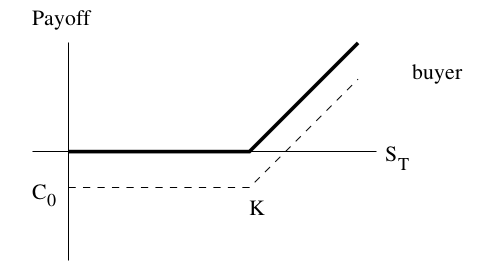
\includegraphics[width=1\linewidth]{Buyer_call} 
		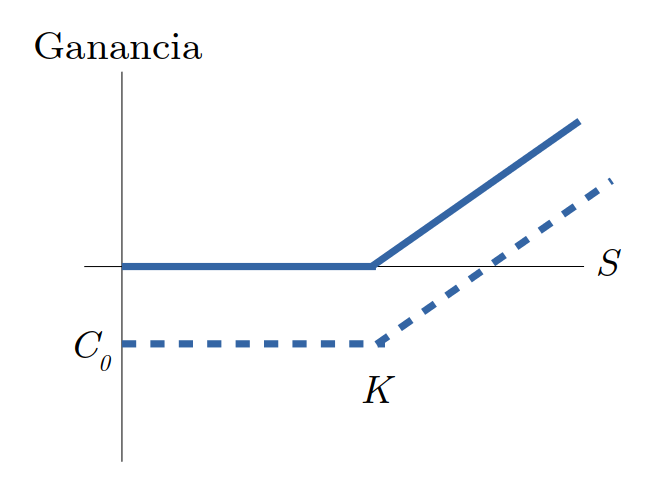
\includegraphics[width=1\linewidth]{Buyer_call_mio} 
		\caption*{Propietario}
		%\label{fig:subim1}
	\end{minipage}
	\begin{minipage}{0.5\textwidth}
		%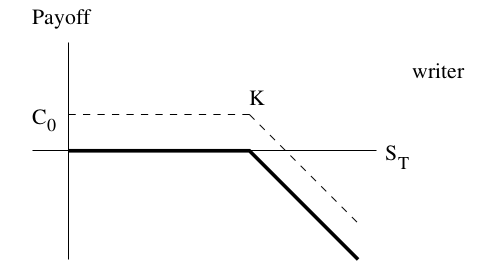
\includegraphics[width=1\linewidth]{Writer_call}
		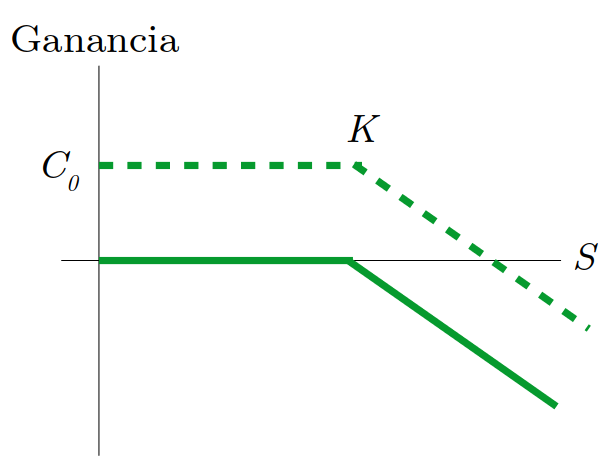
\includegraphics[width=1\linewidth]{Writer_call_mio}
		\caption*{Vendedor}
		
		%\label{fig:subim2}
	\end{minipage}
	\caption{Ganancia opción \textit{call}.}
	\label{graphCall}
\end{figure}

\begin{figure}[h!]
	
	\begin{minipage}{0.5\textwidth}
		\centering
		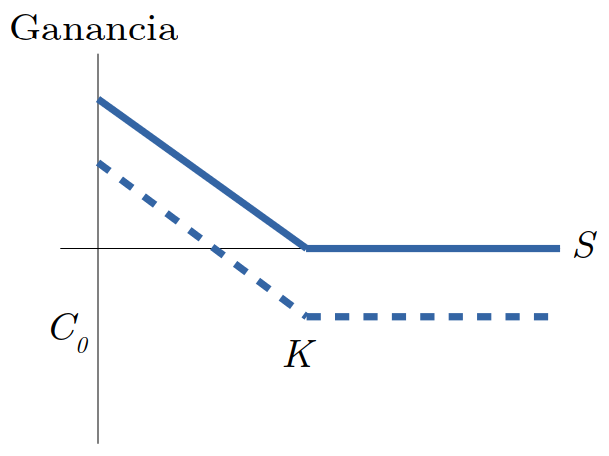
\includegraphics[width=1\linewidth]{Buyer_put_mio} 
		\caption*{Propietario}
		%\label{fig:subim1}
	\end{minipage}
	\begin{minipage}{0.5\textwidth}
		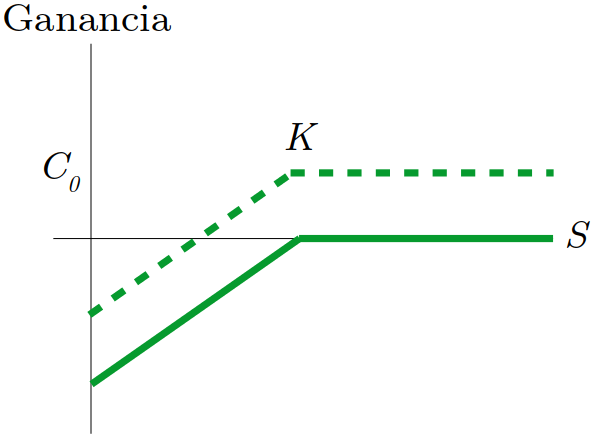
\includegraphics[width=1\linewidth]{Writer_put_mio}
		\caption*{Vendedor}
		%\caption{Tras cuatro iteraciones.}
		
		%\label{fig:subim2}
	\end{minipage}
	\caption{Ganancia opción \textit{put}.}
	\label{graphPut}
\end{figure} 
Uno de los problemas más importantes es determinar de manera única el precio ``justo'' de una opción en un momento determinado para que ambas partes estén de acuerdo. Para más información acerca de conceptos financieros, se pueden consultar \cite{elliot1999mathematics} y el manual para universitarios publicado por la Comisión Nacional del Mercado de Valores.\\

\section{Primer teorema fundamental}
Una vez explicada de manera simplificada el contexto financiero debemos formalizar matemáticamente el modelo del mercado. Para ello, seguimos \cite{elliot1999mathematics}. Fijamos el conjunto de tiempos $ \mathbb{T} = \{0,1,\dots,T\}$ con $ T $ el instante en el que finaliza el modelado de nuestra actividad económica. También fijamos el espacio de probabilidad $ (\Omega, \mathcal{F}, P) $. Este espacio contiene todos los posibles estados del mercado. La información de la que disponen los inversores acerca de la estructura en cada momento $ t \in \mathbb{T}$ viene dada por una sucesión finita y creciente de sub-$ \sigma $-álgebras de $ \mathcal{F} $, $ \mathcal{F}_0 \subset \cdots \subset \mathcal{F}_T = \mathcal{F} $ con $ \mathcal{F}_0 $ trivial, es decir, contiene solamente conjuntos con medida 0 o 1. A este secuencia se le denomina filtración y se denota como $ \mathbb{F} = (\mathcal{F}_t)_{t \in \mathbb{T}} $. El sentido financiero de esta filtración es indicar la información conocida hasta el momento acerca de la evolución de los precios. Por ejemplo, si comenzamos a modelar nuestro mercado hoy, $ \mathcal{F}_0 $ nos aporta únicamente el valor actual. Sin embargo, mañana tendremos la información de los precios en ese momento junto con la obtenida hoy, por lo que es claro que $ \mathcal{F}_0 \subset \mathcal{F}_1  $. También es claro que al llegar al instante final tenemos toda la información acerca del modelo. Llamamos $ d  $ a la dimensión de nuestro mercado, es decir, el número de activos que manejamos. La evolución de los precios de los activos viene dada  por el proceso estocástico $ S = \{S^i_t:\hspace{1mm} t \in \mathbb{T},\hspace{1mm} i=0,\dots,d\} $ donde cada $ S^i_t $ es una variable aleatoria. Todos son activos con riesgos menos el marcado por $ 0 $. Asumimos que el proceso $ S_t^i $ es $ \mathcal{F}_t $-medible para $ i=0,\dots,d $, es decir, se adapta a la filtración $ \mathbb{F} $. Eso significa que para cada $ t \in \mathbb{T} $ se conocen los precios de cada activo hasta ese instante como se ha explicado anteriormente. En general, primero se escoge $ S $ y se toma $ \mathbb{F} $ como la filtración que genera. La tupla $ (\Omega, \mathcal{F}, P, \mathbb{F}, S) $ es la que modela nuestro mercado de valores. \\

El poder adquisitivo de una misma cantidad decrece con el tiempo, consideramos el factor de descuento (o de actualización) en el instante $ t $ dado por $ \beta_t < 1 $ y notamos al valor actual como $ \bar{S}_t = \beta_t S_t $. Sin pérdida de generalidad se puede asumir que $ S^0(0) = 1 $ por lo que podemos expresar todas las unidades en función a dicho valor. En ese caso, el factor $ \beta_t = 1/S^0_t $ es la cantidad de dinero que necesitamos para invertir en bonos en el instante 0 para tener una unidad en el instante $ t $. Podríamos considerar que tomar $ S^0(0) = 1 $  es una simple normalización de los precios. El factor de descuento se puede ver como $ \beta_t = (1+r)^{-t} $. Para entender esta fórmula podemos ver la situación contraria: calcular una cantidad con cierto intereses. De este modo, $ r $ representa el interés considerado o cómo aumentará el valor del dinero en el futuro. Así, el valor de una cantidad $ S $ en el futuro es $ (1+r)S $ considerando solo un paso o $ (1+r)^t S $ si consideramos varios. Por eso, al actualizar pasamos dicho término dividiendo y llegamos a la fórmula de $ \beta_t $ expuesta. Observemos que en ocasiones, como en el caso continuo, el papel de $ (1+r)^t $ es una función exponencial.\\

La cartera de inversión o portafolio para el instante $ t \in \mathbb{T} $ viene dada por la variable aleatoria $ d+1 $ dimensional $ \theta_t = (\theta_t^0,\dots,\theta_t^d) $. Cada $ \theta_t^i $ indica el número de activos del tipo $ i $ que tiene un inversor en el instante $ t $. El valor de la cartera viene determinado por $ V_t(\theta) $ donde
\[
V_0(\theta) = \langle \theta_1 , S_0\rangle, \hspace{2.5mm} V_t(\theta) = \langle \theta_t , S_t\rangle = \sum_{i=0}^{d} \theta_t^i S_t^i \text{ para } \hspace{0.5mm} t \in \mathbb{T}, t \geq 1.
\]
Cada inversor selecciona la cartera de inversión del instante $ t $ una vez se conocen los precios del momento anterior $ t-1 $. La estrategia de inversión $ \theta = \{\theta_t: \hspace{0.5mm}t=1,\dots,T\} $ es el conjunto de todas las carteras de inversión \textit{predecibles}. Decimos que una cartera $ \theta_{t} $ es predecible si depende solamente de los precios de los activos hasta el instante $ t-1 $. Cuando cada cartera de inversión $ \theta_{t+1} $ se puede financiar completamente con las ganancias o pérdidas actuales decimos que la estrategia es \textit{autofinanciada}, es decir, 
\begin{equation*}\label{selfinance}
\langle \theta_{t+1}, S_t \rangle = \langle \theta_{t}, S_t \rangle,
\end{equation*} Notamos $ \Delta X_t = X_t - X_{t-1} $ para cualquier función sobre $ \mathbb{T} $. Si una cartera es autofinanciada, escribimos la ganancia de una cartera de inversión entre los instantes $ (t-1,t] $ como 
\[
\Delta V_t(\theta) = \langle\theta_t, S_t \rangle - \langle\theta_{t-1}, S_{t-1}\rangle = \langle\theta_t, S_t \rangle - \langle\theta_{t}, S_{t-1}\rangle = \langle\theta_{t}, \Delta S_{t}\rangle.
\]
De este modo, la ganancia asociada a la estrategia $ \theta $ hasta el instante $ t $ viene dada por
\[
G_0(\theta) = 0, \hspace{2.5mm} G_t(\theta) = \langle\theta_{1}, \Delta S_{1}\rangle + \cdots + \langle\theta_{t}, \Delta S_{t}\rangle \text{ para } \hspace{0.5mm} t \in \mathbb{T}, t \geq 1.
\]
Vemos entonces que una estrategia es autofinanciada si, y solo si
\begin{equation}\label{selfinifonlyif}
V_t(\theta) = V_0(\theta) + G_t(\theta), \hspace{1mm} \forall t \in \mathbb{T}.
\end{equation}

Destacamos que todas la definiciones anteriores se pueden definir también en base a los valores actualizados $ \bar{S}_t $. \\

También es necesario imponer o aclarar una serie de suposiciones sobre nuestro modelo financiero:
\begin{enumerate}
	\item Ninguna de las transacciones conlleva un coste extra.
	\item Positividad: todos los precios son positivos, es decir,
	\[
	S_t^i > 0 \text{ para } t \in \mathbb{T},\hspace{1mm} i=0,\dots,d.
	\]
	\item Divisibilidad, liquidez y \textit{short selling} (venta en corto): el número de activos que posee un inversor puede ser cualquier valor real. Así,
	\[
	\theta_t^i \in \RR \text{ para } t \in \mathbb{T},\hspace{1mm} i=0,\dots,d.
	\]
	La divisibilidad hace referencia a que $ \theta_t^i $ puede ser una fracción. Claramente, no podemos tener, por ejemplo, media acción. Sin embargo, cuando estamos trabajando con un gran número de acciones podemos considerar que tienen cifras decimales para trabajar con números menores. El hecho de que tome valores en $ \RR $ también significa que podemos comprar o vender el número de acciones deseado, es decir, no imponemos ninguna restricción. Este hecho se conoce como liquidez. Claramente, en mercados reales sí existe dicha restricción en el volumen de las transacciones pero nosotros estamos trabajando con un modelo idealizado. Finalmente, cuando dichos valores son positivos decimos que el inversor tiene una posición larga o \textit{long position}. Si por el contrario estos son negativos, tiene una posición corta o \textit{short position}, por ejemplo, cuando vende algún tipo de bono. Estas acciones se suelen llevar a cabo, por ejemplo, en las denominadas ventas en corto o \textit{short selling} que se usan cuando se prevé que un determinado activo va a bajar de valor. Así, suponemos que tenemos una acción cuyo precio actual es 100 cuyo valor suponemos que va a disminuir. Antes de que baje más, la vendemos, es decir, tomamos una posición \textit{short}. Pasado un periodo de tiempo, la acción bajan a 70 por lo que tomamos una posición \textit{long} y las compramos de nuevo. De este modo, tenemos las misma cantidad de activos que al principio pero hemos obtenido un beneficio de 70. En estas operaciones también corremos el riesgo de perder dinero ya que es posible que el valor de los activos crezca en vez de disminuir. 
	
	\item Solvencia: el valor de todas las carteras de inversión debe ser siempre positivo,
	\[
	V_t (\theta) \geq 0\text{ para todo } t \in \mathbb{T}.
	\]
	En este caso, decimos que la cartera es \textit{admisible}. A la clase de estrategias autofinanciadas y admisibles la denotaremos como $ \Theta_a $.
	\item El espacio $ \Omega $ es finito, es decir, las variables aleatorias $ S_t^i $ no pueden tomar infinitos valores. Así, tenemos que $ \Omega = \{ \omega_1,\dots,\omega_n\} $.
\end{enumerate}

Ya tenemos el modelo financiero sobre el que vamos a trabajar. Exponemos ahora unos resultados que nos servirán posteriormente para probar el teorema principal del capítulo.
\bigskip
%% Parecido Prop 4.1 del otro libro Mathematics for finance
%% LEMMA 2.2.1
\begin{lemaBox}\label{2.2.1}
	Dada $ V_0 $ una función $ \mathcal{F}_0 $-medible y para $ d \in \NN  $ sean los procesos reales y predecibles $ \theta^1,\dots,\theta^d $, el único proceso predecible $ \theta^0 $ que convierte a $ \theta = (\theta^0,\theta^1,\dots,\theta^d) $ en una estrategia autofinanciada con valor $ V_0 (\theta)= V_0 $ viene dado por
	\[
	\theta^0_t = V_0 + \sum_{i=1}^{t-1}(\theta^1_i\Delta\bar{S}^1_i+\cdots+\theta^d_i\Delta\bar{S}^d_i) - (\theta^1_t\bar{S}^1_{t-1}+\cdots+\theta^d_t\bar{S}^d_{t-1}).
	\]
\end{lemaBox}
\begin{proof}
	Claramente $ \theta^0 $ es predecible. Para ver que la estrategia es autofinanciada, por \eqref{selfinifonlyif} solo necesitamos ver que $ \theta^0_t $ es la única solución predecible de la ecuación 
	\begin{equation*}
	\begin{split}
	\bar{V}_t(\theta) &= \theta^0_t + \theta^1_t\bar{S}^1_t+\cdots+\theta^d_t\bar{S}^d_t \\
	&= V_0 + \sum_{i=1}^{t}(\theta^1_i\Delta\bar{S}^1_i+\cdots+\theta^d_i\Delta\bar{S}^d_i)
	\end{split}
	\end{equation*}
\end{proof}
\bigskip
Introducimos ahora el concepto de \textit{viabilidad}, esencial para lo que sigue. Decimos que un mercado es viable si para toda estrategia admisible y autofinanciada no contiene ninguna oportunidad de arbitraje. La ausencia de arbitraje significa que si el valor inicial de una cartera de inversión es $ V_0(\theta) = 0 $ entonces $ V_T(\theta) = 0 $ con probabilidad 1 para toda $ \theta \in\Theta_a $. La viabilidad del mercado impone la siguiente restricción.

\bigskip
%% LEMMA 3.2.1
\begin{lemaBox}\label{3.2.1}
	Si el modelo de mercado es viable, las ganancias actualizadas a cualquier proceso predecible $ \hat{\theta} \in \RR ^d $ no pueden pertenecer a 
	\[
	C = \{Y \in \RR^n: Y_i \geq 0\text{ para } i=1,\dots,n \text{ y } \exists i \text{ tal que } Y_i > 0\}.
	\]
\end{lemaBox}
\begin{proof}
	En primer lugar vemos que $ C $ es el octante positivo de $ \RR^n $ sin el origen, que claramente es un cono y es convexo. La ausencia de arbitraje significa que para toda estrategia admisible $ \theta \in \Theta_a $ tal que $ V_0(\theta) = 0 $ entonces
	\[
	\bar{V}_t(\theta) = \bar{G}_t (\theta) \notin C.
	\]
	Por el lema \ref{2.2.1}, dados los procesos predecibles $ \hat{\theta} = (\theta^1, \dots,\theta^d) $, existe un único proceso real $ \theta^0 $ tal que $ \theta = (\theta^0, \theta^1,\dots, \theta^d) $ es autofinanciada y $ V_0(\theta) = 0 $. Las ganancias con los valores actualizados viene dada por
	\[
	\bar{G}_t(\hat{\theta}) = \sum_{j=1}^{t} \langle \theta_j, \Delta \bar{S}_j \rangle =   \sum_{j=1}^{t} \left( \sum_{i=1}^{d} \theta_j^i \Delta \bar{S}_j^i  \right).
	\]
	Supongamos que $ \bar{G}_t(\hat{\theta}) \in C $; si $ \beta_T $ denota el factor de descuento en el instante $ T $,
	\[
	V_T(\theta) = \beta_T^{-1} \bar{V}_t(\theta) = \beta_T^{-1}(V_0 (\theta) + \bar{G}_t(\theta)) = \beta_T^{-1}\bar{G}_t(\theta).
	\]
	Vemos entonces que $ V_T(\theta) $ es no negativa y estrictamente positiva con probabilidad no nula, lo que contradice la viabilidad al existir arbitraje.
\end{proof}
\bigskip
Nuestro objetivo es caracterizar la viabilidad de un mercado en términos de los incrementos de $ \bar{S} $. Para ello son necesarias las martingalas.
\bigskip
\begin{definicion}
	Un proceso $ \mathbb{F} $-adaptado $ M = (M_t)_{t\in \mathbb{T}} $ es una $ ( \mathbb{F},P)$-mar\-tingala si $ E(|M_t|) < \infty $ para todo $ t \in \mathbb{T} $ y 
	\[
	E(M_{t+1}|\mathcal{F}_t) = M_t \textit{ para todo } t \in \mathbb{T}\setminus{T}.
	\]
	Si $ M = (M_t) $ es una martingala y $ \phi = (\phi_t)_{t\in \mathbb{T}} $ es un proceso predecible en $ (\Omega, \mathcal{F}, P, \mathbb{F}, S) $ entonces al proceso $ X = \phi \cdot M $ dado por
	\[
	X_0=0, \hspace{2mm}X_t = \phi_1\Delta M_1+\cdots+ \phi_t\Delta M_t \hspace{1.5mm} t \geq1
	\]
	se le denomina martingala transformada de $ M $ por $ \phi $.
\end{definicion}

Notamos que $ M $ es una martingala si, y solo, si
\[
E(\Delta M_{t+1} |\mathcal{F}_t ) = 0 \text{ para todo } t\in \mathbb{T}\setminus\{T\}.
\]
También es importante destacar que, por la linealidad de la esperanza, cualquier combinación lineal de martingalas es una martingala. \\

Que los precios en el mercado sigan una martingala no debe de ser extraño. Recordemos que para $ t \in \mathbb{T} $, $ \mathcal{F}_t $ indica la cantidad de información acerca de los precios de los activos hasta dicho momento. Por lo tanto, la esperanza condicionada solo nos indica que estamos calculando el valor esperado a partir de lo que conocemos hasta ahora. Además, para que el mercado sea ``justo'', dicho valor en el futuro debería ser, en media, el que tenemos ahora. \\

El siguiente resultado es meramente técnico y nos servirá posteriormente. 

\bigskip
%% THEOREM 2.3.5
\begin{teoremaBox}\label{2.3.5}
	Un proceso real $ M $ es una martingala si, y solo si, 
	\[
	E((\phi \cdot M)_t) = E(\sum_{i=1}^{t}\phi_i\Delta M_i) = 0, \hspace{1mm} \forall t \in \mathbb{T}\setminus\{0\}
	\]
	para todo proceso $ \phi $ predecible y acotado.
\end{teoremaBox}
\begin{proof}
	Si $ M $ es un martingala, también lo es la tranfomada $ X = \phi \cdot M $ y $ X_0 =0 $ ya que
	\[
	E(\Delta X_{t+1}|\mathcal{F}_t) = E(\phi_{t+1}\Delta M_{t+1}|\mathcal{F}_t) =  \phi_{t+1} E(\Delta M_{t+1}|\mathcal{F}_t) = 0.
	\] 
	Por ello, $ E((\phi \cdot M)_t) = 0 $ para todo $ t \geq 1 $ en $ \mathbb{T} $.
	Demostremos ahora la otra implicación. Para $ s > 0 $, sea $ A \in \mathcal{F}_s $ y definimos el proceso predecible $ \phi $ como $ \phi_{s+1} = 1_A $ y $ \phi_t = 0 $ para el resto de $ t\in \mathbb{T} $. Entonces, para $ t > s $ se tiene que
	\[
	0 = E((\phi \cdot M)_t) = E(1_A(M_{s+1}-M_s)).
	\]
	Como es cierto para todo $ A \in \mathcal{F}_s $, se cumple que $ E(\Delta M_{s+1} | \mathcal{F}_s) = 0 $ por lo que $ M $ es una martingala.
\end{proof}
\bigskip
Nos encontramos ahora un contexto general donde no asumimos que el modelo sea finito o que $ \mathbb{F} $ sea generada por $ S $. Supongamos que el proceso de los precios actualizados $ \bar{S} $ es una martingala bajo una probabilidad $ Q $, esto es:
\[
E_Q (\Delta \bar{S}^i_t | \mathcal{F}_{t-1}) = 0, \text{ para } t \in \mathbb{T}\setminus \{0\} \text{ e } i = 0,\dots,d,
\]
donde $ E_Q $ significa la esperanza respecto de la probabilidad (medida) $ Q $. Sea $ \theta \in \Theta_a $ una estrategia admisible tal que los procesos de los precios actualizados son integrables respecto a $ Q $. Por \eqref{selfinifonlyif} tenemos que:
\begin{equation*}
\begin{split}
\bar{V}_t(\theta) &= V_0(\theta) + \bar{G}_t(\theta) \\
&= \langle \theta_{1}, S_0 \rangle + \sum_{u=1}^{t} \langle \theta_{u}, \Delta \bar{S}_u \rangle \\
&= \sum_{i=1}^{d}(\theta_1^i S_0^i + \sum_{u=1}^{t} \theta_{u}^i \Delta \bar{S}_u^i).
\end{split}
\end{equation*}
Vemos entonces que $ \bar{V}(\theta) $ es una constante más una suma finita de martingalas transformadas, por lo que también es una martingala con valor inicial $ V_0 (\theta) $. Entonces, tenemos que: \[ E(\bar{V}_t (\theta)) = E(V_0 (\theta)) = V_0(\theta) .\] 
Esta situación imposibilita la existencia de arbitraje. Si sabemos de antemano que los procesos de los precios actualizados son integrables respecto a $ Q $, supongamos que $ V_0 (\theta) = 0$ y $ V_T (\theta) \geq 0$ casi seguramente (respecto a $ Q $). Como $ E_Q = (\bar{V}_t ( \theta)) = 0 $ se sigue que $ V_T(\theta) = 0$ casi seguramente (respecto a $ Q $). Esto sigue siendo verdadero casi seguramente para $ P $, demostrando que $ P $ y $ Q $ tienen los mismos conjuntos vacíos. Llegamos entonces a la siguiente definición:
\bigskip
\begin{definicion}
	Una probabilidad $ Q $ que sea equivalente a $ P $ como media $ (Q\sim P) $ es una medida martingala equivalente (EMM) para $ S $ si el proceso de los precios actualizados $ \bar{S} $ es una martingala bajo $ Q $ para la filtración $ \mathbb{F} $. Es decir, para cada $ i =0,\dots, d $ tenemos que $ \bar{S}^i $ es una $ (\mathbb{F},Q) $-martingala.
\end{definicion}
\bigskip
Todo lo presentado anteriormente, nos aporta el siguiente resultado que acabamos de demostrar:
\bigskip
\begin{proposicionBox}\label{martThenViab}
	Si existe una medida martingala equivalente para $ S $, entonces el modelo de mercado discreto es viable, es decir, no contiene ninguna oportunidad de arbitraje.	
\end{proposicionBox}
\bigskip
El recíproco de esta afirmación es cierto, tal y como exponemos en el siguiente teorema que es el objetivo final de este capítulo y en el que usaremos el teorema de la alternativa de Gordan en forma equivalente del teorema de separación establecido en el corolario \ref{coroSep}. Recibe el nombre de ``primer teorema fundamental de asignación de precios''.
\bigskip
\begin{teoremaBox}(Primer reorema fundamental de asignación de precios)\label{VIABLEiofEMM}
	Un modelo de mercado discreto es viable si, y solo si, existe una medida de martingala equivalente para $ S $.
\end{teoremaBox}
\begin{proof}
	Ya sabemos por la proposición \ref{martThenViab} que la existencia de una medida de martingala equivalente garantiza la viabilidad del modelo por lo que solo tenemos que probar la otra implicación. \\
	
	Suponemos entonces que el modelo es viable. Necesitamos construir una medida $ Q \sim P $ en la que los precios son martingalas relativas a la filtración $ \mathbb{F} $. Sea $ C $ es el cono convexo de todas las variables aleatorias reales $ \phi $ en $ (\Omega, \mathcal{F}) $ tales que $ \phi(\omega) \geq 0 $ casi seguramente y $ \phi(\omega_i) > 0 $ para al menos un $ \omega_i = \Omega = \{\omega_i,\dots, \omega_n \} $. Asumimos $ p_i = P(\{\omega_i\}) > 0 $. Por el lema \ref{3.2.1}, hemos visto que para un mercado viable debemos tener $ \bar{G}_t(\hat{\theta}) \notin C$ para todos los procesos predecibles $ \hat{\theta} \in  \RR^d $. Por otro lado, el conjunto definido por tales ganancias 
	\[
	L = \{\bar{G}_t(\hat{\theta}):\hspace{0.5mm} \hat{\theta}=(\theta^1,\dots,\theta^d),\text{ con } \theta^i \text{ predecible para } i=1,\dots,d \},
	\]
	es un subespacio vectorial del espacio de todas las funciones reales y  $ \mathcal{F} $-medibles en $ \Omega $. Como $ L $ y $ C $ son disjuntos, podemos separar $ L $ y el subconjunto compacto de $ C $ definido como $ K =\{X\in C: \hspace{0.5mm} E_P(X) = 1\} $ gracias al corolario \ref{coroSep}. Sea $ \xx^0 \in \RR^d $ el elemento que proporciona dicho resultado. Tomamos $ \xi_i = (0,\dots,\frac{1}{p_i},\dots,0) $ para $ i \leq n $. Vemos que $ E_P(\xi_i) = \frac{p_i}{p_i} = 1$ por lo que $ \xi_i \in K $ y $ \langle \xx^0, \xi_i \rangle = \frac{x^0_i}{p_i} > 0$. Por ello, $ x^0_i > 0$ para todo $ i=1,\dots,n $.
	
	Definimos ahora el funcional lineal $ g(\xx) = \frac{\langle \xx^0, \xx\rangle}{\alpha} $ donde $ \alpha = \sum_{i=1}^{n} x^0_i$. Sea $ p^* \in \RR^d$ un vector con $ p^*_i = \frac{x_i^0}{\alpha} $ por lo que $ \sum_{i=1}^{n} p^*_i = 1 $. Usamos el vector $ p^* $ para inducir una probabilidad $ P^* $ en $ \Omega = \{\omega_1,\dots,\omega_n\} $ haciendo $ P^*(\{\omega_i\}) = p^*_{i} > 0 $. Veamos que $ P^* $ es la martingala equivalente deseada. En efecto, sea $ E^*(\cdot) $ que denota la esperanza relativa a $ P^* $. Nuevamente, por el corolario \ref{coroSep}, tenemos que $ g(\xx) = \frac{1}{\alpha}\langle \xx^0,\xx\rangle = 0$ para todo $ \xx\in L $. En particular, esta situación se da para  para $ \bar{G}_T (\hat{\theta}) $ con $ \hat{\theta}=(\theta^1,\dots,\theta^d) $ un vector de procesos predecibles por lo que.
	\[ E^*(\bar{G}_T (\hat{\theta})) = 0.\]
	Hemos conseguido una estrategia auto-financiada $ \theta $ con $ V_0(\theta) = 0 $. Como $ \bar{V}_t (\theta) = V_0(\theta) + \bar{G}_T (\theta)$, implica que $ E^*(\bar{V}_t (\theta)) = 0 $ para cada $ \theta $. Por el lema \ref{2.2.1} podemos generar tal $ \theta $ para cada proceso predecible de $ n $  dimensiones. En particular, lo podemos hacer para $ (0,\dots, \theta^i,\dots,0) $ donde $ i\leq n $. Por lo tanto
	\[
	E^*(\sum_{t=1}^{T}\theta_t^i\Delta \bar{S}^i_t) = 0
	\]
	se da para cada proceso predecible y acotado $ (\theta^i)_{i=1,\dots,T} $. El teorema \ref{2.3.5} implica que cada $ S^i $ es una martingala bajo $ P^* $. Por ello, $ P^* \sim P $.
\end{proof}
\bigskip
\input{capitulos/aplicación.tex}

\part{Procesamiento de nubes de puntos generadas por escáner láser}
\chapter{Iterative Closest Point (ICP)}
	\thispagestyle{empty}
	
	\newcommand{\ii}{\textbf{\emph{i}}}
	\newcommand{\jj}{\textbf{\emph{j}}}
	\newcommand{\kk}{\textbf{\emph{k}}}
	\newcommand{\qq}{\textbf{\emph{q}}}
	\newcommand{\pp}{\textbf{\emph{p}}}
%	\newcommand{\vv}{\textbf{\emph{v}}}
%	\newcommand{\xx}{\textbf{\emph{x}}}
%	\newcommand{\uu}{\textbf{\emph{u}}}
%	\newcommand{\ww}{\textbf{\emph{w}}}
%	\newcommand{\aaa}{\textbf{\emph{a}}}
	\newcommand{\nn}{\textbf{\emph{n}}}
%	\newcommand{\bb}{\textbf{\emph{b}}}
	
	\paragraph{}En esta sección explicaremos el primer algoritmo denominado \textit{Iterative Closest Point} (ICP), o Iteración del Punto más Cercano. Este algoritmo se utiliza en la etapa de alineación y su finalidad es que todas las tomas de datos estén referenciadas respecto al mismo sistemas de coordenadas. Este proceso también se suele denominar \textit{registro de datos} o \textit{data registration}. Veremos el método inicial propuesto en $ 1\,992 $ por Paul J.Besl and Neil D.MacKay \cite{ICPBesl}. Como veremos, este es un algoritmo complejo en tiempo y por ello, se tarda bastante en obtener los resultados deseados. Por ello, una vez estudiado el algoritmo se propondrán unas pequeñas mejoras del mismo que consistirán, básicamente, en el uso de las normales en cada punto para acelerar el proceso.\\
	
	Antes de explicar el algoritmo necesitamos unas nociones previas acerca de los \textit{cuaternios}. Los utilizaremos para la representación de las rotaciones en tres dimensiones, frente a la forma tradicional de representación matricial, y serán de gran ayuda a la hora de demostrar la convergencia del algoritmo. Tanto para la explicación de los cuaternios como su 
	uso en optimización se ha tomado como referencia \cite{QuatYan}.
\begin{figure}[h!]
	\begin{minipage}{0.5\textwidth}
		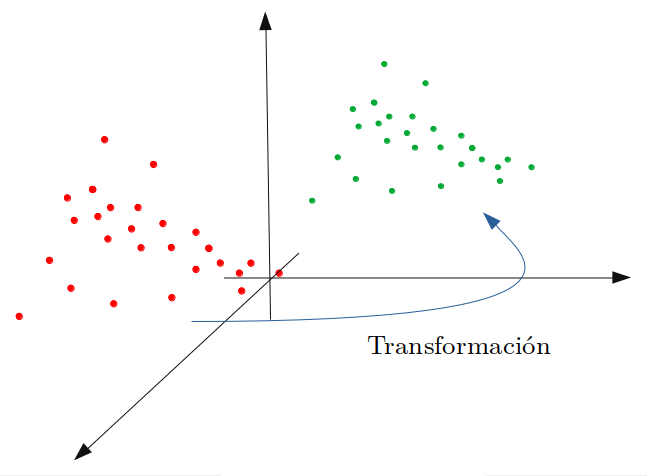
\includegraphics[width=0.8\linewidth, height=4.5cm]{Otros/Ej_Alineado_1} 
		%\caption*{Vista 1}
		%\label{fig:subim1}
	\end{minipage}
	\begin{minipage}{0.5\textwidth}
		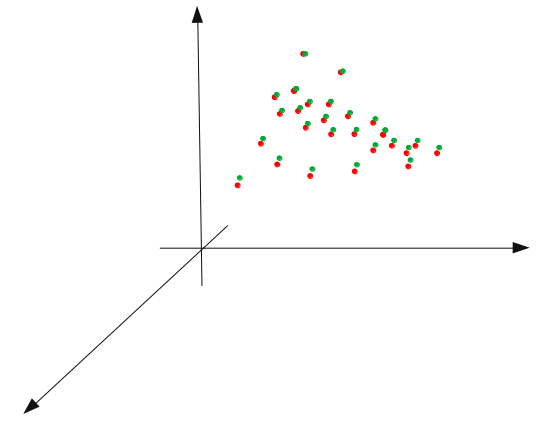
\includegraphics[width=0.8\linewidth, height=4.5cm]{Otros/Ej_Alineado_2}
		%\caption*{Vista 2}
		%\label{fig:subim2}
	\end{minipage}
	\caption{Antes y después de alinear dos nubes de puntos.}
\end{figure}

	\section{Cuaternios}
		Su desarrollo se atribuye a W.R Hamilton en $ 1\,843 $.  Son una extensión de los números complejos. Mientras que estos últimos solo incluyen la unidad imaginaria $ \ii$, los cuaternios añaden las unidades imaginarias $ \ii, \jj, \kk $ tales que:
		\begin{equation*}
			\ii^2 = \jj^2 = \kk^2 = \ii\jj\kk = -1.
		\end{equation*} 
		
		Así, el conjunto de los cuaternios se define como:
		\begin{equation*} 
			\lbrace q_0 + q_1 \ii + q_2 \jj + q_3 \kk : q_0, q_1, q_2, q_3 \in \RR \rbrace.
		\end{equation*}
		Podemos ver a los cuaternios como la suma de un escalar $ q_0 \in \RR$ y de un vector de $ \RR^3 $ que llamamos $ \qq = (q_1,q_2,q_3)$ donde la base usual de $ \RR^3 $ viene dada por los vectores unitarios $ \ii =(1,0,0), \jj = (0,1,0) \text{ y } \kk = (0,0,1)$. Notaremos $
		q = q_0 + \qq =  q_0 + q_1 \ii + q_2 \jj + q_3 \kk $. Si la parte escalar es 0, es decir, $ q_0 = 0 $ hablamos de un \textit{cuaternio puro}. Por otro lado, a modo de notación podemos expresar $ q $ como vectores de cuatro dimensiones, es decir, si $ q $ es de la forma mencionada podemos pensar que $ q = (q_0, q_1, q_2, q_3) \in \RR^4 $.
		
		\begin{subsection}{Suma y producto}
			La suma de dos cuaternios se realiza componente a componente. Por ello, dados los cuaternios
		 	\begin{equation*}
		 	\begin{split}
		 	q &= q_0 + q_1 \ii + q_2 \jj + q_3 \kk = q_0 + \qq \\
		 	p &= p_0 + p_1 \ii + p_2 \jj + p_3 \kk = p_0 + \pp,
		 	\end{split}
		 	\end{equation*}
			definimos su suma de la siguiente manera:
			
			\begin{equation*}
			q + p= (q_0 + p_0 )+ (q_1 + p_1 )\ii + (q_2 + p_2 ) \jj + (q_3 + p_3 ) \kk.
			\end{equation*}
			Es directo comprobar que la suma es asociativa y conmutativa.\\
			
			El producto, por su parte, sigue una serie de reglas introducidas por Hamilton y que las presentamos a continuación:
			\begin{equation*}
			\begin{split}
			\ii^2 &= \jj^2 = \kk^2 = \ii\jj\kk = -1.\\
			\ii\jj &= 	\kk = 	-\jj\ii.\\
			\jj\kk &= \ii = -\kk\jj. \\
			\kk\ii &= 	\jj = -	\ii\kk.
			\end{split}
			\end{equation*}
			Por ello, el producto de dos cuaternios viene dado por:
			\begin{equation*}
			\begin{split}
			pq&= (p_0 + p_1 \ii + p_2 \jj + p_3 \kk)(q_0 + q_1 \ii + q_2 \jj + q_3 \kk) \\
			&= p_0q_0 - (p_1q_1+p_2q_2+p_3q_3) + p_0(q_1\ii+q_2\jj+q_3\kk) \\
			&+ q_0(p_1\ii+p_2\jj+p_3\kk) + (p_2q_3-p_3q_2)\ii +  (p_3q_1-p_1q_3)\jj \\
			&+ (p_1q_2-p_2q_1)\kk.
			\end{split}
			\end{equation*}
			Podemos simplificar esta expresión usando el producto escalar y vectorial de $ \RR^3 $ quedando la expresión más concisa:
			\[
			pq = p_0q_0 - \langle \pp , \qq \rangle + p_0\qq + q_0\pp + \pp \times \qq.
			\]			
			No es difícil comprobar que el producto es asociativo y distributivo respecto a la suma pero no conmutativo. La no conmutatividad se puede observar del hecho de que el producto vectorial no es conmutativo. Es importante notar que los cuaternios son cerrados bajo la suma y el producto definidos anteriormente. En el caso del producto, obtenemos otro cuaternio con parte escalar $ p_0q_0 -  \langle \pp , \qq \rangle $ y vector $ p_0\qq + q_0\pp + \pp \times \qq $. \\
			
			Este conjunto con las operaciones de suma y producto forman un anillo no conmutativo. El elemento neutro para la suma sería un cuaternio donde $ q_0 = q_1 = q_1 = q_3 = 0 $ y dado un elemento $  q = q_0 + \qq $ su opuesto sería $ -q = -q_0-\qq  $. Por su parte, el elemento neutro para el producto sería un cuaternio con parte real $ 1 $ y vector $ \mathbf{0} $.
		\end{subsection}
	
		\subsection{Conjugado, norma e inverso}
			Sea el cuaternio dado por $ q = q_0 + q_1 \ii + q_2 \jj + q_3 \kk $. Notamos a su \textit{conjugado} como $ q^* $ y que se define como:
			\[
			q^* = q_0 - \qq = q_0 - q_1 \ii - q_2 \jj - q_3 \kk.
			\]
			
			De la definición obtenemos las siguientes propiedades básicas del manejo de cuaternios:
			\begin{equation*}
			\begin{split}
			(q^*)^* &= q - (-\qq) = q.\\
			q + q^* &= q_0.\\
			 q q^*= q^*q & = (q_0+\qq)(q_0+\qq) \\
			&= q_0q_0 - \langle-\qq, \qq \rangle + q_0\qq + (-\qq)q_0 + (-\qq) \times \qq \\
			&= q_0^2 + \langle\qq , \qq \rangle\\
			&= q_0^2 + q_1^2 + q_3^2 + q_4^2 \\
			& = q_0^2 + \norm{\qq}.
			\end{split}
			\end{equation*}
			En la última expresión $ \norm{\cdot} $ representa la norma usual de $ \RR^3 $. Podemos probar que dados dos cuaternio $ p,q $ se cumple que $ (pq)^* = q^*p^* $. Efectivamente:
			\begin{equation*}
			\begin{split}
			(pq)^* &= p_0q_0 - \langle \pp , \qq \rangle - p_0\qq - q_0\pp - \pp \times \qq \\
			 &= p_0q_0 - \langle \pp , \qq \rangle - p_0\qq - q_0\pp + \qq \times \pp \\
			 &= q_0p_0 - \langle -\qq , -\pp \rangle + q_0(-\pp)+p_0(-\qq) + (-\qq) \times (-\pp)\\
			 &= (q_0-\qq)(p_0-\pp)\\
			 &= q^* p^*.
			\end{split}
			\end{equation*}
			
			La \textit{norma} de un cuaternio se nota como $ \abs{q} $ y se define como $ \abs{q} = \sqrt{q^*q}$. Usando la propiedad anterior de que el conjugando del producto es el producto de los conjugados cambiados de orden llegamos a:
			\begin{equation*}
			\begin{split}
			\abs{pq}^2 &= (pq)^*(pq) \\
			&= q^*p^*pq \\
			&=  q^*\abs{p}^2 q \\
			&= \abs{p}^2q^*q \\
			&= \abs{p}^2\abs{q}^2.
			\end{split}
			\end{equation*}
			
			Por su parte, el \textit{inverso} de un cuaternio se define como:
			\[
			q^{-1} = \frac{q^*}{\abs{q}^2}.
			\]
			Se cumple que: 
			\[
			qq^{-1} =q^{-1}q =  \frac{q^*}{\abs{q}^2} q = \frac{\abs{q}^2}{\abs{q}^2} = 1.
			\]
			En el caso de que $ q $ sea unitario (tenga norma uno) tenemos que $ q^{-1} = q^* $. Notar que los cuaternios unitarios forman un grupo con operación interna el producto. 
			
	
		\subsection{Cuaternios y rotaciones}\label{Cuat+Rot}
		El grupo de rotaciones en $ \RR^3 $ alrededor de un eje que pasa por el origen, y que lo notamos como $ SO(3) $, está formado por las matrices reales 3x3 que son ortogonales (su inversa coincide con la traspuesta) y tienen determinante igual a 1. \\
		
		Nos surge entonces la siguiente pregunta: ¿por qué usar los cuaternios para representar dichas rotaciones? En primer lugar, el uso de matrices resulta redundante. Las rotaciones en $ \RR^3 $ tienen básicamente tres grados de libertad: dos para la representación del eje (dado en coordenadas esféricas, por ejemplo) y uno para el ángulo de giro. Por ello, al usar matrices estamos usando demasiados elementos. Con el uso de los cuaternios seguimos teniendo redundancia pero solo por un valor más. Además, a partir de un eje de rotación y un ángulo de giro se puede construir fácilmente el cuaternio asociado, y del mismo modo, obtener el eje y ángulo a partir del cuaternio, mientras que en matrices dicha relación no es tan clara.  También reducimos el número de operaciones necesarias a la hora de componer dos rotaciones. En la multiplicación de matrices se necesitan 27 multiplicaciones y 18 sumas y en el producto de cuaternios (veremos que esta es la operación de composición) 16 multiplicaciones y 20 sumas. Por otro lado, podemos usar los \textit{ángulos de Euler} para identificar las rotaciones que utiliza el número de valores mínimo. Sin embargo, con este sistema podemos llegar a una situación no deseada que se conoce como \textit{gimbal lock} o \textit{bloqueo del cardán} \cite{QuatPowerPoint}.  Este fenómeno se produce cuando los tres ejes están en el mismo plano y nos produce la pérdida de uno de los ejes de giro. Por estas razones, entre otras, los cuaternios se conocen generalmente como la ``mejor'' manera para representar las rotaciones en el espacio. Más específicamente, la representación de las rotaciones en tres dimensiones se hace mediante cuaternios unitarios. Veamos el proceso: \\
		
		Sea $ q $ un cuaternio unitario de la forma $ q = q_0 + \qq $. Al tener norma uno tenemos que $ \abs{q}^2 = q_0^2 + \norm{\qq}^2 = 1 $. Así, como $ (q_0, \norm{\qq}) \in \mathbb{S}^1 $, existe un único ángulo $ \theta \in \lbrack 0,2\pi ) $ que cumple: 	
		\begin{equation*}
			\begin{cases}
			 \cos^2 \theta = q_0^2 \\
			 \sen^2\theta = \norm{\qq}^2 ,
			\end{cases}
		\end{equation*}
		y podemos escribir ahora $ q $ en términos de $ \theta \text{ y } \uu$ con $ \uu = \mathbf{\qq}/\norm{\qq}$ de la siguiente manera: $ q = \cos\theta + \uu\sen\theta $. \\
		
		Dado el cuaternio unitario $ q $, definimos la aplicación $ L_q $ dada por:
		\begin{equation*}
			\begin{split}
			L_q:\RR^3 &\longrightarrow \RR^3 \\
			\vv &\longmapsto L_q(\vv) = q\vv q^* =(q_0^2-\norm{\qq}^2)\vv + 2\langle\qq , \vv\rangle \qq + 2q_0(\qq \times \vv)
			\end{split}
		\end{equation*} 
		La aplicación $ L_q $ está bien definida y no tenemos problema en multiplicar un vector por un cuaternio, ya que podemos ver un vector como un cuaternio puro. Hacemos ahora dos observaciones interesantes que nos hacen pensar, en principio, que la aplicación $ L_q $ actúa como una rotación con eje $ \qq $.
	
		\bigskip
		\begin{observacion}
			La aplicación $ L_q $ no cambia la norma de $ \vv \in \RR^3 $.
		\end{observacion}
		En efecto:	
		\begin{equation*}
			\norm{L_q(\vv)} = \norm{q\vv q^*} = \abs{q} \norm{\vv} \abs{q^*} = \norm{\vv}.
		\end{equation*}
		
		\begin{observacion}\label{NoCambiaEje}
			Si $ \vv = k\qq $ con $ k \in \RR $ entonces la dirección de $ \vv $ no cambia al aplicarle $ L_q $.
		\end{observacion}	
		Usando la definición de $ L_q $ y al ser $ q $ unitario llegamos a:
		\begin{equation*}
		\begin{split}
		L_q(\vv) &= q \vv q^* \\
		&= (q_0^2-\norm{\qq}^2)(k\qq) + 2\langle\qq, k\qq\rangle\qq + 2q_0(\qq \times k\qq) \\
		&= k(q_0^2-\norm{\qq}^2)\qq + 2k\langle\qq, \qq\rangle\qq + 2kq_0(\qq \times \qq) \\
		&= k(q_0^2-\norm{\qq}^2)\qq + 2k\norm{\qq}^2\qq \\
		&= k(q_0^2+\norm{\qq}^2)\qq \\
		&= k\qq.
		\end{split}
		\end{equation*}
		\bigskip
		
		Antes de formalizar la ``intuición'' que nos han dado las observaciones anteriores necesitamos otra que es un poco más técnica. 
	
		\bigskip
		\begin{observacion}
			La aplicación $ L_q $ es lineal, es decir, dados $ a_1,a_2 \in \RR \text{ y } \vv_1, \vv_2 \in \RR^3$ se tiene que $ L_q(a_1\vv_1 + a_2 \vv_2) = a_1 L_q (\vv_1) + a_2 L_q(\vv_2) $.
		\end{observacion}
		Se obtiene por la distributividad del producto:
		\begin{equation*}
		\begin{split}
		L_q(a_1\vv_1 + a_2 \vv_2 ) &=q(a_1\vv_1 + a_2 \vv_2)q^* \\
		&=q(a_1\vv_1 q^* + a_2 \vv_2 q^*) \\
		&=qa_1\vv_1 q^*  + qa_2 \vv_2 q^*\\
		&= a_1q\vv_1 q^*  + a_2 q\vv_2 q^* \\
		&=a_1 L_q (\vv_1) + a_2 L_q(\vv_2).
		\end{split}			
		\end{equation*}
		\bigskip
		
		El teorema que exponemos a continuación es clave y nos indica que dado un vector y ángulo podemos construir un cuaternio $ q $ tal que $ L_q $ representa la rotación deseada.
		
		\begin{teoremaBox}
			Para cualquier cuaternio $ q = q_0 + \qq = \cos \theta/2 + \uu \sen \theta/2$ y para cualquier vector $ \vv \in \RR^3 $ tenemos que $ L_q(\vv) $ es equivalente a la rotación con eje de giro $ \uu $ y ángulo $ \theta $. 
		\end{teoremaBox}
	
\begin{proof}
Tomamos $ \vv \in \RR^3 $ y lo expresamos en términos de $ \qq $ y $ \lbrace\qq \rbrace^\perp $. De este modo, $ \vv = \aaa + \nn $ donde $ \aaa $ es la componente respectiva a $ \qq $ y $ \nn $ la de $ \lbrace\qq \rbrace^\perp $. Bajo $ L_q $, $ \aaa $ se queda invariante por la observación \ref{NoCambiaEje} mientras que $ \nn $ rota un ángulo $ \theta $ alrededor de $ \qq $. En efecto:
\begin{equation*}
	\begin{split}
	L_q(\nn) &= (q_0^2-\norm{\qq}^2)\nn + 2\langle\qq , \nn\rangle\qq + 2q_0(\qq \times \nn)\\
		&= (q_0^2-\norm{\qq}^2)\nn + 2q_0(\qq \times \nn) \\
		&= (q_0^2-\norm{\qq}^2)\nn + 2q_0\norm{\qq}(\uu \times \nn),
			\end{split}
			\end{equation*} 	
			donde la última igualdad se debe a que $ \uu = \qq / \norm{\qq} $. Notamos $ \nn_0= \uu \times \nn$. Es claro por ello que $ \nn_0 $ es perpendicular tanto a $ \uu $ (y por ello también a $ \qq $) y a $ \nn $. Obtenemos: 
			\begin{equation}\label{fmla}
				L_q(\nn) =  (q_0^2-\norm{\qq}^2)\nn + 2q_0\norm{\qq}\nn_0.
			\end{equation} 
			Tanto $ \nn_0 \text{ como }  \nn $ tienen la misma longitud:
			\begin{equation*}
				\norm{\nn_0} = \norm{\nn \times \uu} = \norm{\uu \times \nn} = \norm{\nn}\norm{\uu}\sen(\pi/2) = \norm{\nn}.
			\end{equation*}
			Escribimos \ref{fmla} es términos de $ \theta $:
			\begin{equation*}
			\begin{split}
			L_q(\nn) &= (\cos^2\frac{\theta}{2} - \sen^2\frac{\theta}{2})\nn + (2\cos^2\frac{\theta}{2}\sen^2\frac{\theta}{2})\nn_0 \\
			&= \cos\theta\nn + \sen\theta\nn_0.
			\end{split}
			\end{equation*}
			Las últimas igualdades se han obtenido mediante las fórmulas del seno y coseno del ángulo doble. Vemos que el vector resultante es la rotación de $ \nn $ un ángulo $ \theta $ en el plano definido por $ \nn \text{ y } \nn_0 $. Claramente el vector resultante es perpendicular al eje de rotación, ya que $ \nn$ y $ \nn_0 $ pertenecen a $ \lbrace \qq \rbrace ^\perp$. La demostración termina usando la linealidad que nos aporta la observación 3.
		\end{proof}
	 	\bigskip
	 	
En resumen, dados $ \qq \in \RR^3$ y $ \theta \in \RR$ representamos la rotación de ángulo de giro $ \theta $ alrededor del eje $ \qq$ por $  q = \cos\frac{\theta}{2} + \frac{\qq}{\norm{\qq}} \sen \frac{\theta}{2} $ y la aplicamos a un vector $ \uu \in \RR^3 $ mediante $ L_{q} (\uu) = q\uu q^* $.  \\
		
		Finalmente, exponemos la siguiente observación que nos indica la relación de la composición de rotaciones con su representación mediante cuaternios.
		\bigskip
		\begin{observacion}
			 Sean p,q dos cuaternios unitarios, entonces $ L_q \circ L_p = L_{qp} $. 
		\end{observacion}
		Como $ p \text{ y } q$ son unitarios entonces $ pq $ también lo es. Notamos $ L_p(\uu) = \vv \text{ y } L_q(\vv) = (L_q \circ L_p)(\uu) = \ww $. Obtenemos:
		\begin{equation*}
		\begin{split}
			\ww &= L_q(\vv) = q\vv q^* \\
			&= q(p\uu p^*) q^*\\ 
			&= (qp)\uu(qp)^* \\ 
			&= L_{qp}(\uu).
		\end{split}
		\end{equation*} 
		\bigskip
		
		De este modo, hemos obtenido que la composición de rotaciones representadas en cuaternios se obtiene mediante la multiplicación de los cuaternios que representa cada una de las rotaciones por separado. \\
				
	
	\section{Cuaternios y optimización}\label{optimizacion}
Sea $ P = \{\pp_i\} $ un conjunto con $ N_p $ puntos que queremos alinear tomando como sistema de referencia otro conjunto $ X = \{\xx_i\} $ de tamaño $ N_x $. Suponemos que $ N_p = N_x $ y que cada $ \pp_i \in P $ corresponde con $ \xx_j \in X $ siempre y cuando $ i = j $. Esta correspondencia hace referencia a que conocemos cómo se relacionan los puntos de ambos conjuntos y por ello $ p_i $ es el punto $ x_i $ pero en un sistema de referencia diferente. Aclararemos esta relación en apartados siguientes. Suponer que ambos conjuntos de puntos tienen el mismo tamaño puede parecer bastante restrictivo en un primer momento pero posteriormente veremos que no es el caso. De este modo, el problema consiste en encontrar una rotación $ R $ y una traslación $ \bb $ que nos proporcionen las distancias más pequeñas entre los puntos. Así, la función objetivo a ser minimizada es:
		
		\begin{equation}\label{min}
		F (R,\bb) = \sum_{i = 1}^{N_p} \norm{R\pp_i + \bb - \xx_i}^2.
		\end{equation}
		En primer lugar, obtenemos los centroides de ambos conjuntos de puntos. Recordando que $ N_p = N_x $, los notamos como:
		\[
		\bar{\pp} = \frac{1}{N_p} \sum_{i=i}^{N_p} \pp_i,  \quad \bar{\xx} = \frac{1}{N_p} \sum_{i=i}^{N_p} \xx_i.
		\]
		A continuación, obtenemos las coordenadas relativas a los centroides:
		\[
		\pp_i' = \pp_i - \bar{\pp}, \quad \xx_i' = \xx_i - \bar{\xx}.
		\]
		Notamos que se cumple que:
		\begin{equation}\label{cen0}
		\begin{split}
			\sum_{i=1}^{N_p} \pp_i' = \sum_{i=1}^{N_p} (\pp_i - \bar{\pp}) = \sum_{i=1}^{N_p} \pp_i - N_p\bar{\pp} = \sum_{i=1}^{N_p} \pp_i - N_p\frac{1}{N_p} \sum_{i=i}^{N_p} \pp_i = 0, \\
			\sum_{i=1}^{N_p} \xx_i' = \sum_{i=1}^{N_p} (\xx_i - \bar{\xx}) = \sum_{i=1}^{N_p} \xx_i - N_p\bar{\xx} = \sum_{i=1}^{N_p} \xx_i - N_p\frac{1}{N_p} \sum_{i=i}^{N_p} \xx _i = 0. 
		\end{split}
		\end{equation}		
		Expresando ahora \eqref{min} en términos de $ \pp_i, \xx_i, \bar{\pp} \text{ y } \bar{\xx}$:
		\begin{equation*}
		\begin{split}
		\sum_{i = 1}^{N_p} \norm{R\pp_i + \bb - \xx_i}^2 &= \sum_{i = 1}^{N_p} \norm{R(\pp_i' + \bar{\pp} ) + \bb - (\xx_i' + \bar{\xx})}^2 \\
		&=\sum_{i = 1}^{N_p} \norm{R\pp_i' -\xx_i' + R\bar{\pp}  + \bb - \bar{\xx}}^2 \\
		&= \sum_{i = 1}^{N_p} \langle R\pp_i' -\xx_i' + R\bar{\pp}  + \bb - \bar{\xx}, R\pp_i' -\xx_i' + R\bar{\pp}  + \bb - \bar{\xx} \rangle.
		\end{split}
		\end{equation*} 
		Para simplificar la escritura, llamamos $ a_i = R\pp_i' -\xx_i' \text{ y } c = R\bar{\pp}  + \bb - \bar{\xx}$. Como el producto escalar es bilineal obtenemos: 
		\begin{equation*}
		\begin{split}
		\sum_{i = 1}^{N_p} \langle a_i + c, a_i + c\rangle &= \sum_{i = 1}^{N_p} \langle a_i + c, a_i \rangle + \sum_{i = 1}^{N_p} \langle a_i + c, c\rangle\\ 
		& = \sum_{i = 1}^{N_p} \langle a_i, a_i \rangle + \sum_{i = 1}^{N_p} \langle c, a_i\rangle + \sum_{i = 1}^{N_p} \langle a_i, c \rangle + \sum_{i = 1}^{N_p} \langle c, c\rangle \\
		& = \sum_{i = 1}^{N_p} \norm{a_i}^2 + 2\sum_{i = 1}^{N_p} \langle a_i, c\rangle + \sum_{i = 1}^{N_p} \norm{c}^2 \\
		& = \sum_{i = 1}^{N_p} \norm{a_i}^2 + 2\sum_{i = 1}^{N_p} \langle a_i, c\rangle + N_p \norm{c}^2 \\
		& = \sum_{i = 1}^{N_p} \norm{a_i}^2 + 2 \langle \sum_{i = 1}^{N_p} a_i, c\rangle + N_p \norm{c}^2.
		\end{split}
		\end{equation*} 
		Si sustituimos $ a_i $ por su valor en el término central y usamos \eqref{cen0}:
		\begin{equation*}
			\sum_{i = 1}^{N_p} a_i = \sum_{i = 1}^{N_p} (R\pp_i' -\xx_i') = \sum_{i = 1}^{N_p} R\pp_i' - \sum_{i = 1}^{N_p}\xx_i' = 0.
		\end{equation*} 
		Por lo tanto: 
		\begin{equation*}
		\begin{split}
		\sum_{i = 1}^{N_p} \norm{R\pp_i + \bb - \xx_i}^2 &= \sum_{i = 1}^{N_p} \norm{R\pp_i' -\xx_i'}^2 + N_p\norm{R\bar{\pp}  + \bb - \bar{\xx}}^2.
		\end{split}
		\end{equation*} 
		La traslación $ \bb $ buscada debería hacer 0 el segundo término obteniendo entonces:
		\[\bb =- R\bar{\pp}  + \bar{\xx}.
		\]
		Ahora, para obtener la mejor rotación utilizamos el primero término. Reescribiendo la misma llegamos a:
		\begin{equation*}
		\begin{split}
		\sum_{i = 1}^{N_p} \norm{R\pp_i' -\xx_i'}^2 &= \sum_{i = 1}^{N_p} \langle R\pp_i' -\xx_i', R\pp_i' -\xx_i' \rangle \\
		&= \sum_{i=1}^{N_p} \langle R \pp_i' , R \pp_i' \rangle - 2\sum_{i=1}^{N_p}\langle R\pp_i', \xx_i'\rangle + \sum_{i=1}^{N_p} \langle \xx_i', \xx_i'\rangle \\
		&= \sum_{i=1}^{N_p} RR^T \norm{\pp_i'}^2 - 2\sum_{i=1}^{N_p}\langle R\pp_i', \xx_i'\rangle + \sum_{i=1}^{N_p} \norm{\xx_i'}^2\\
		&= \sum_{i=1}^{N_p} (\norm{\pp_i'}^2 + \norm{\xx_i'}^2)- 2\sum_{i=1}^{N_p}\langle R\pp_i', \xx_i'\rangle.
		\end{split}
		\end{equation*}
		El primer término no depende de la rotación por lo que no influirá en el cálculo. Y el segundo, que sí depende de $ R $, hará que  $ \sum_{i = 1}^{N_p} \norm{R\pp_i' -\xx_i'}^2 $ sea mínimo cuando tome su valor máximo al estar restando. Nos encontramos ahora en un problema de maximización. Usamos ahora la representación en cuaternios de las rotaciones y que hemos introducido en la sección \ref{Cuat+Rot}. Sea $ q  $ el cuaternio (unitario) que representa la misma rotación que la matriz $ R $. Tenemos que maximizar:
		
		\begin{equation*}
		\sum_{i=1}^{N_p}\langle q\pp_i'q^*, \xx_i'\rangle.
		\end{equation*}
		Aplicando la definición del producto de cuaternios no es difícil probar que: 
		%%% (¡¡ REVISAR PROCEDIMIENTO !!):
		
		\begin{equation}\label{1.4}
		\sum_{i=1}^{N_p}\langle q\pp_i'q^*, \xx_i'\rangle = 	\sum_{i=1}^{N_p}\langle q\pp_i', \xx_i'q\rangle.
		\end{equation}
		Visto $ q $ como un vector de $ \RR^4 $ tenemos que $ q = (q_0, q_1, q_2, q_3)^T$. También vemos los puntos $ \pp_i' $ y $ \xx_i' $ como cuaternios puros notando a sus componentes como $ \pp_i' = (0, p_{i1}', p_{i2}', p_{i3}' ) $ y $ \xx_i' = (0, x_{i1}', x_{i2}', x_{i3}' ) $ para $ i=1,...,N_p $.\\
		
		Nuestro propósito ahora es escribir los sumandos de \eqref{1.4} como producto matricial. Construimos las matrices para cada $ i= 1, \dots, N_p$: 
		%%% (¡¡ VER CÓMO SE CONSTRUYEN!!):
		
		\begin{equation}\label{covDife}
		P_i = \begin{pmatrix}
		0 & -p_{i1}' &-p_{i2}' &-p_{i3}' \\
		p_{i1}' & 0 & p_{i3}'& -p_{i2}' \\
		p_{i2}' & -p_{i3}' & 0 & p_{i1}' \\
		p_{i3}' & p_{i2}' & -p_{i1}' & 0\\
		\end{pmatrix}
		\text{, }
		X_i = \begin{pmatrix}
		0 & -x_{i1}' &-x_{i2}' &-x_{i3}' \\
		x_{i1}' & 0 & -x_{i3}'& x_{i2}' \\
		x_{i2}' & x_{i3}' & 0 & -x_{i1}' \\
		x_{i3}' & -x_{i2}' & x_{i1}' & 0\\
		\end{pmatrix}.
		\end{equation}	
		Observamos que $ q\pp_i' $ coincide con $ P_i q$  y que $ \xx_i'q $ hace lo mismo con $ X_i q $, sustituimos en \eqref{1.4}:
		\begin{equation*}
		\begin{split}
		\sum_{i=1}^{N_p}\langle q\pp_i', \xx_i'q\rangle &=  \sum_{i=1}^{N_p}\langle P_i q,  X_ix\rangle\\
		&= \sum_{i=1}^{N_p} \langle q ,P_i^T X_i q \rangle\\
		&= \langle q , \left( \sum_{i=1}^{N_p}P_i^T X_i\right) q \rangle.
		\end{split}
		\end{equation*}
		Podemos comprobar sin dificultad que la matriz $ P_i^T X_i $ es simétrica por lo que la suma de ellas también lo es. Llameamos a su suma
		\begin{equation}\label{MSum}
			M = \sum_{i = 1}^{N_p}P_i^TX_i.
		\end{equation}
 Como $ M $ es simétrica podemos asegurar que todos sus valores propios son reales. Sean $ \lambda_1 \geq \lambda_2 \geq \lambda_3 \geq \lambda_4 $ dichos valores propios (tenemos en cuentas las multiplicidades) y $ \vv_1, \vv_2, \vv_3, \vv_4 $ sus correspondientes vectores propios unitarios asociados. Sabemos que vectores propios asociados a diferentes valores propios son perpendiculares entre sí. Si corresponden al mismo podemos elegirlos de tal manera para que también sean ortogonales.  Por lo tanto, podemos escribir el cuaternio $ q $ como combinación lineal de vectores propios:
		\[
		q = \alpha_1 \vv_1 + \alpha_2 \vv_2 + \alpha_3 \vv_3 + \alpha_4 \vv_4,
		\]
		tenemos entonces que la matriz $ M $ expresada en la base $ \{ \vv_1, \vv_2, \vv_3, \vv_4\} $ de sus vectores propios es diagonal  con $ M = diag(\lambda_1, \lambda_2, \lambda_3, \lambda_4) $. Así:
		\begin{equation*}
		\begin{split}
		\langle q , M q \rangle &= \langle \alpha_1 \vv_1 + \alpha_2 \vv_2 + \alpha_3 \vv_3 + \alpha_4 \vv_4, M(\alpha_1 \vv_1 + \alpha_2 \vv_2 + \alpha_3 \vv_3 + \alpha_4 \vv_4 )\rangle \\
		&=  \langle \alpha_1 \vv_1 + \alpha_2 \vv_2 + \alpha_3 \vv_3 + \alpha_4 \vv_4, \lambda_1\alpha_1 \vv_1 + \lambda_2\alpha_2 \vv_2 + \lambda_3\alpha_3 \vv_3 + \lambda_4\alpha_4 \vv_4 \rangle \\
		&=  \lambda_1\alpha_1^2 + \lambda_2\alpha_2^2 + \lambda_3\alpha_3^2 + \lambda_4\alpha_4^2.
		\end{split}
		\end{equation*}
		De este modo, 
		%%%(USAR LEMA 2.1 MATEMÁTICAS ??) 
		$ \langle q , M q \rangle $ es máximo cuando $ \alpha_1^2 = 1 $ y $ \alpha_2^2 = \alpha_3^2 = \alpha_4^2 = 0 $ ya que al ser $ q $ unitario debe cumplir $ \alpha_1^2 + \alpha_2^2 + \alpha_3^2 + \alpha_4^2 = 1$. Así, el cuaternio que maximiza \eqref{1.4} es el vector propio asociado al máximo valor propio de M.
		
\section{Algoritmo ICP}\label{algICP}
Una vez explicadas las herramientas que intervienen en el proceso de minimización de la función (\ref{min}), explicamos el algoritmo tal y como fue propuesto por Paul J.Besl and Neil D.MacKay. Destacamos una sutil diferencia entre la construcción original y la que nosotros hemos presentado. Besl and MacKay identifican la matriz $ M $ que hemos definido en (\ref{MSum}) como:
\begin{equation}\label{matCov}
M = Q(\Sigma_{px}) =
 \begin{pmatrix}
tr(\Sigma_{px}) & \Delta^t \\
\Delta & \Sigma_{px} + \Sigma_{px}^t + tr(\Sigma_{px})I_3\\
\end{pmatrix}, 
\end{equation}
donde 
\[
\Sigma_{px} = \frac{1}{N_p}\sum_{i=1}^{N_p} \lbrack (\pp_i-\bar{\pp})(\xx_i - \bar{\xx})^t\rbrack, \]
\[A_{ij} = (\Sigma_{px}-\Sigma_{px}^t)_{ij} \quad i,j \in \lbrace 0,1,2 \rbrace,\]
y 
\[\Delta = \begin{pmatrix}
A_{12} & A_{20} & A_{01}  \\
\end{pmatrix}. \]
No es difícil comprobar que ambas definiciones son equivalentes haciendo la construcción elemento a elemento. Destacar que se han presentado estas dos definiciones de la misma matriz, ya que la dada por (\ref{MSum}) es más fácil de comprender en el proceso de minimización. Por su parte, (\ref{matCov}) será la que se implementará en el código del algoritmo al ser la propuesta original. \\

Así, con todo los mecanismos a nuestra disposición, la solución propuesta para alinear ambas nubes de puntos es la siguiente:
\begin{enumerate}
\item Sea el conjunto de puntos $ P $ a alinear con el modelo $ X $. Notar que no tienen porqué tener el mismo tamaño.
\item Inicializaremos el conjunto $ P_0 = P $. Para la iteración $ k \geq 0$, repetir a), b) y c) hasta que haya convergencia con una tolerancia $ \tau $.
\begin{enumerate}
	\item Calcular el conjunto de $ Y_k  $ de los puntos más cercanos de $ P_k $ respecto a $ X $. Notamos como $ e_{k} $ a la distancia media entre $ Y_k  $ y $ P_k  $ obtenida mediante (\ref{min}).
	\item Aplicar el método de optimización de la distancia media (sección \ref{optimizacion}) para obtener los cuaternios $ qT_{k} $ y $ qR_{k} $. 
	\item Obtener el conjunto $ P_{k+1} = R(qR_{k})P_0 + qT_{k} $. Calcular $ d_k $ que nota la distancia media entre $ Y_k  $ y $ P_k+1  $ obtenida mediante (\ref{min}).
	\item Terminar cuando $ d_{k-1} - d_k < \tau $.
\end{enumerate}
\end{enumerate}

En el pseudocódigo hemos notado como $  R(qR_{k}) $ a la rotación asociada al cuaternio $ qR_{k} $ de la iteración k-ésima. Notar que cada $ y_{i,k} $ es el punto más cercano asociado a $ p_{i,k} $ para $ i = 1,\dots, N_p $. De este modo, queda clara la nota que apuntamos al inicio de la sección y es que podemos suponer que los conjuntos tienen el mismo número de puntos, ya que el proceso no se realiza con el modelo $ X $ sino con el conjunto de puntos más cercanos. \\
 
Exponemos ahora el teorema que nos asegura la convergencia del método sugerido, que en este caso es convergencia local. Esto nos impondrá una serie de restricciones que explicaremos más adelante.

\bigskip
\begin{teoremaBox}
El algoritmo ICP siempre converge de manera monótona a un mínimo local respecto de la función objetivo distancia media.
\end{teoremaBox}
\begin{proof}
Tenemos el conjunto $ P_0 $ que queremos ajustar al modelo $ X $. Sea $ P_k = R(qR_{k-1})P_0 + qT_{k-1}$ el conjunto de puntos transformados al principio de la iteración $ k $ y sea $ Y_k $ el conjunto de puntos más cercanos a cada punto con $ y_{i,k} $ el punto más cercano asociado a $ p_{i,k} $ para $ i = 1,\dots, N_p $ que hemos calculado. Definimos:
\[
e_k = \frac{1}{N_p} \sum_{i=1}^{N_p} \norm{ y_{i,k}-p_{i,k}}.
\]
Aplicamos el proceso explicado en la sección \ref{optimizacion} y obtenemos $ qT_{k} $ y $ qR_{k} $. Calculamos:
\[
d_k = \frac{1}{N_p} \sum_{i=1}^{N_p} \norm{ y_{i,k}-R(qR_{k})p_{i,k}-qT_{k}}.
\]
Afirmamos que $ d_k \leq e_k $ para la iteración k-ésima. De lo contrario, si $ d_k > e_k $ tendríamos que la distancia media del conjunto inicial es menor que la distancia media tras aplicar el proceso descrito de optimización lo cual es imposible por la propia construcción del mismo. \\

En la siguiente iteración, calculamos $ P_{k+1} = R(qR_{k})P_k + qT_{k} $. Obtenemos ahora el $ Y_{k+1} $ y $ e_{k+1} $ igual que en la anterior iteración. Es evidente que $ e_{k+1} \leq d_k $ por la propia definición de $ Y_{k+1} $. Notar que para toda iteración $ k $ se cumple $ e_k, d_k \geq 0 $ al ser la suma de números no negativos por lo que hemos conseguido la siguiente relación:
\[
0\leq d_{k+1} \leq e_{k+1} \leq d_k \leq e_k
\]

Finalmente como la sucesión $ \{d_k\}_{k \geq 1} $ es decreciente y acotada podemos afirmar que es convergente y como consecuencia que el método converge de manera monótona a un mínimo local.
\end{proof}

\bigskip

Una vez demostrada la convergencia del método, es necesario recalcar una serie de observaciones acerca del mismo.
\bigskip

\begin{observacion}
Al converger a un mínimo local es necesario una fase de prealineado
\end{observacion}
La demostración del método asegura que el método es convergente pero no nos aporta el elemento al que converge. Por ello, al aplicar el método podemos llegar a una situación donde el procedimiento converja a una mejora en la transformación  pero no sea la que nosotros deseamos. Necesitamos entonces la fase de \textit{prealineado}. Este proceso se puede llevar a cabo de diferentes maneras. La más habitual es dar manualmente una serie de puntos clave que se correspondan en los dos conjuntos y aplicar una transformación de acuerdo a los mismos. Tenemos así una primera aproximación de ambos conjuntos de puntos para asegurar que la convergencia se produce a la situación que deseamos. En nuestro caso, dicho procedimiento se ha implementado del siguiente modo:


\begin{enumerate}
\item Escoger de cada conjunto tres puntos que se encuentren en ambos y sean fácilmente identificables al pertenecer a una esquina, tener el mismo color, etc. Estos puntos deben de estar ordenados de la misma forma en ambos casos, es decir, el primer punto seleccionado de un conjunto debe ``coincidir'' con el primero del otro. Igual con los dos restantes. Este proceso se recoge en la figura \ref{fig:ex-pre}.

\begin{figure}[h!]
		\begin{subfigure}{0.5\textwidth}
			\centering
			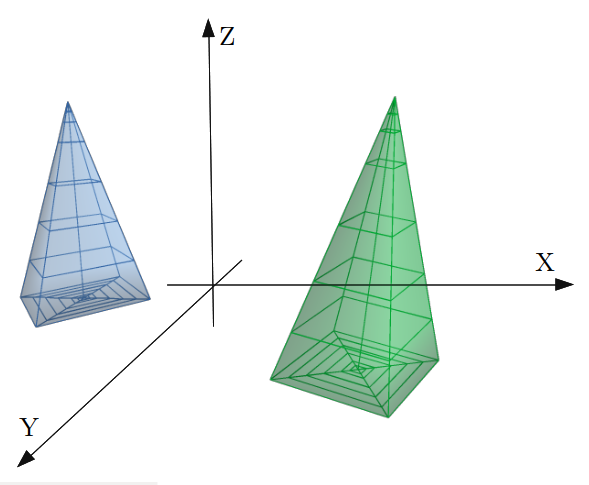
\includegraphics[width=0.8\linewidth, height=4.5cm]{Otros/PRE_1} 
			\caption{}
			%\label{fig:subim1}
		\end{subfigure}
		\begin{subfigure}{0.5\textwidth}
			\centering
			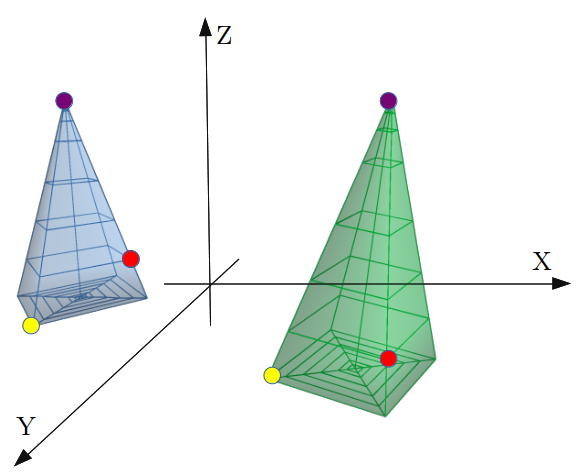
\includegraphics[width=0.8\linewidth, height=4.5cm]{Otros/PRE_2}
			\caption{}
			%\label{fig:subim2}
		\end{subfigure}	
		\caption{Selección de puntos en ambos conjuntos.}
		\label{fig:ex-pre}
\end{figure}
\item Llevar los primeros puntos seleccionados al origen de coordenadas.

\item Llevar los segundos a la parte positiva del eje $ X $ manteniendo fijos los anteriores.
\item Intentar aproximar lo máximo posible los otros puntos mediante una rotación alrededor del eje $ X $.
\end{enumerate}

\begin{figure}[h!]
	\begin{subfigure}{0.5\textwidth}
		\centering
		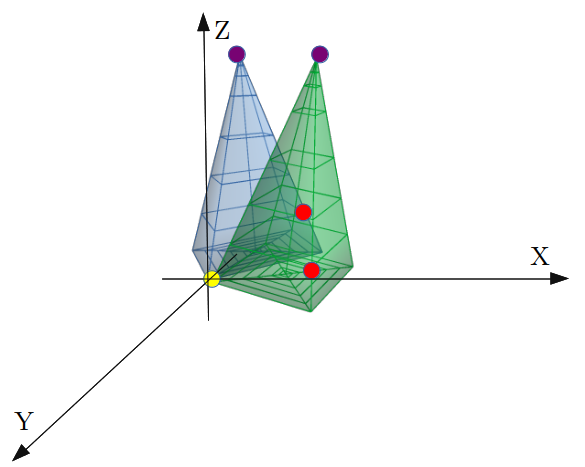
\includegraphics[width=0.8\linewidth, height=4.5cm]{Otros/PRE_3}
		\caption{Paso 2: llevar los primeros puntos al origen.}
	\end{subfigure}
	\begin{subfigure}{0.5\textwidth}
		\centering
		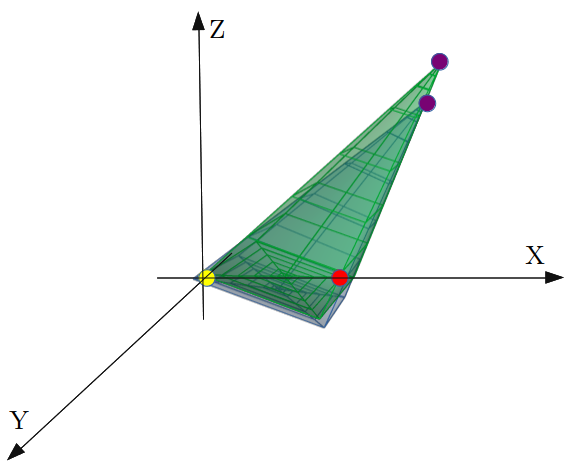
\includegraphics[width=0.8\linewidth, height=4.5cm]{Otros/PRE_4}
		\caption{Paso 3: llevar los segundos puntos al eje $ X $.}
	\end{subfigure}
	\begin{center}
		\begin{subfigure}{0.5\textwidth}
			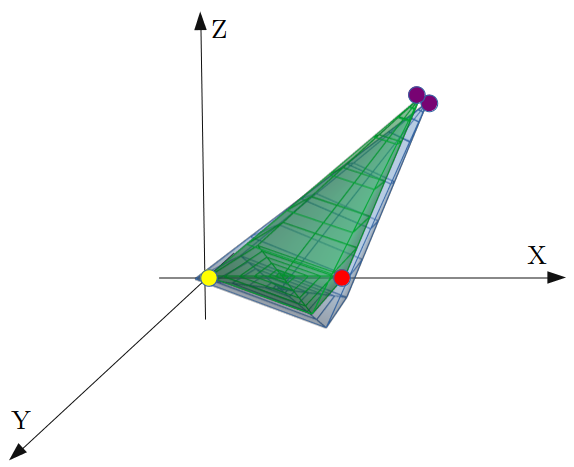
\includegraphics[width=0.8\linewidth, height=4.5cm]{Otros/PRE_5}
			\caption{Paso 4: aproximar lo máximo posible el punto restante.}
		\end{subfigure}
	\end{center}		
	\caption{Mecanismo de prealineado a partir de tres puntos.}
	\label{fig:ex-pre2}
\end{figure}


La figura \ref{fig:ex-pre2} muestra el proceso a seguir en estos últimos pasos. En secciones posteriores veremos un ejemplo práctico de este procedimiento.

\bigskip 
\begin{observacion}\label{ObsTmp}
El cálculo de los puntos más cercanos entre las nubes de puntos es un proceso muy costoso en tiempo.
\end{observacion}
Este paso del algoritmo es el que más tiempo ocupa de todo el proceso al tener una complejidad O($ N_p^2 $) en el peor de los casos. También tenemos que tener en cuenta el tamaño de los conjuntos de los puntos. La finalidad de este proceso es tener un modelo digital detallado y fiel a la realidad de un objeto real. Ello conlleva que las tomas se realicen con cierta calidad lo que hace que, incluso en modelos relativamente pequeños, cada una ronde los 2 millones de puntos. Si es un modelo más complejo podríamos llegar a los 20 millones. En estas situaciones, aplicar el método tradicional podría durar horas en completarse. \\

En esta situación, nos planteamos la posibilidad de una variante para no tener que comprobar todos y cada uno de los puntos en el proceso. En una primera aproximación, podríamos pensar en coger un subconjunto aleatorio de puntos de cada toma y aplicar el proceso descrito. Sin embargo,  comprobamos que esta solución no es válida. Esto se debe a la convergencia local del método lo que nos conduce a las situaciones indeseadas que queremos evitar con el prealineado. Por ello, nos tenemos que plantear mecanismos más complejos que aseguren que se tienen en cuenta las tomas completas. \\

Un primer método sería usar índices espaciales como los \textit{octrees}. Los \textit{octrees} son estructuras jerárquicas que dividen el espacio en cubos denominados \textit{voxels}. Cada \textit{voxel} puede contener un máximo número de puntos por lo que si se supera dicho número el \textit{voxel} se dividiría en otros \textit{voxels} más pequeños. También podríamos imponer una profundidad máxima del árbol. En esta situación, solo deberíamos comprobar la distancia con un punto de cada \textit{voxel} y una vez se tiene, filtrar los puntos del modelo por esa distancia. \\

Otro mecanismo sería identificar alguna característica que nos permita clasificar los puntos. Como las tomas corresponden al mismo modelo, podemos suponer que la característica que buscamos se mantienen en cierta medida en ambos casos y solo tenemos que buscar el punto más cercano con aquellos que tienen características similares. Esta será la opción que nosotros usaremos para proponer alternativas basadas en este procedimiento y que veremos en la sección \ref{varNormal} .
\bigskip

\section{Ejemplos prácticos}\label{ejemPrac1}
En esta sección procedemos a probar el método implementado. Empezamos con un ejemplo parecido al artículo original. Los conjuntos de puntos para la prueba son:

\begin{table}[h!]
	\centering
	\begin{tabular}{| c | c | c |} 
		\hline
		$ x_1 $ & $ x_2 $ & $ x_3 $ \\
		\hline
		0.4389 & -0.0588 & 1.0699 \\ 
		0.4202 & 0.2052 & 1.1252 \\
		0.4201 &0.2539 & 1.1325 \\
		0.4495 & 0.0469 & 1.1260  \\
		0.4412 & 0.1796 & 1.1515 \\
		0.4826 & -0.0137 & 1.1359  \\
		0.4628 & 0.0703 & 1.1458 \\
		0.4700 & 0.1852 & 1.1765 \\
		\hline
	\end{tabular}
	\caption{Conjunto 1.}
	\label{table:1}
\end{table}

\begin{table}[h!]
	\centering
	\begin{tabular}{| c | c | c |} 
		\hline
		$ y_1 $ & $ y_2 $ & $ y_3 $ \\
		\hline
		0.7278 &0.0712 & 1.4610 \\ 
		0.7019 & 0.2480 & 1.4867 \\
		0.7621 & 0.1828 & 1.4720 \\
		0.7271 & 0.1769 & 1.4809  \\
		0.7067 & 0.0462 & 1.495 \\
		0.6438 & -0.0540& 1.4359  \\
		0.7247 & -0.0116 & 1.4385 \\
		0.6982 & 0.1981 & 1.4832 \\
		0.7700 & 0.2500 & 1.5000 \\
		0.8000 & -0.100 & 1.400 \\
		0.8300 & 0.3000 & 1.4500 \\
		\hline
	\end{tabular}
	\caption{Conjunto 2.}
	\label{table:2}
\end{table}

En la imagen \ref{fig:ICP_1} se muestran los puntos antes y después de aplicar una iteración de ICP. Notar que los del primer conjunto se han dibujado de color rojo y los del segundo de color verde. En esta ocasión no ha sido necesaria la etapa de prealineado al no haber una situación deseada tras la transformación. \\

\begin{figure}[h!]
	
	\begin{subfigure}{0.5\textwidth}
		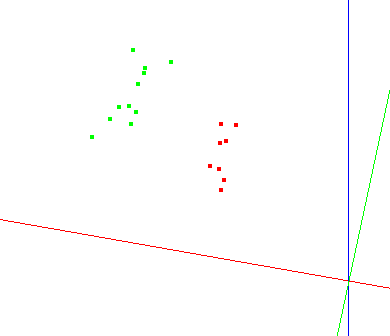
\includegraphics[width=0.7\linewidth, height=4cm]{ICP/prueba_ICP_1_1} 
		%\caption{Caption1}
		%\label{fig:subim1}
	\end{subfigure}
	\begin{subfigure}{0.5\textwidth}
		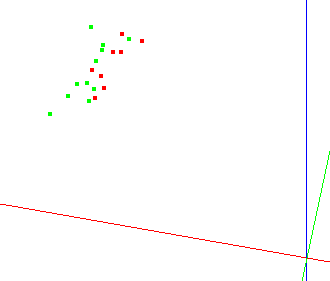
\includegraphics[width=0.7\linewidth, height=4cm]{ICP/prueba_ICP_1_2}
		%\caption{Caption 2}
		%\label{fig:subim2}
	\end{subfigure}
	
	\caption{Conjuntos de puntos antes y después de una iteración de ICP.}
	\label{fig:ICP_1}
\end{figure}

Según los datos calculados, la distancia media en milímetros ha pasado de 403.3571 a 61.0297. El tiempo que ha tardado en realizar el proceso es de 0.00226548 segundos. La traslación y rotación expresada como cuaternio vienen dadas por 
\[
q_T =  (\text{0.166271}, \text{ 0.165485}, \text{ 0.349303})
\]
y 
\[
q_R = (\text{0.0234481}, \text{ 0.0238614}, \text{ -0.154144}, \text{ 0.987482}).
\]

%%Besl y McKay también aportan en su artículo una estimación del la cantidad de operación necesarias en este caso. Para estos conjuntos con 8 y 11 puntos respectivamente ..... COMPRENDER. ¿Es necesario?. \\

El segundo ejemplo que vamos a probar consiste en un caso real, concretamente dos tomas de una escultura de un pie perteneciente a la Facultad de Bellas Artes de la Universidad de Granada tomadas con un escáner láser Faro Focus 130. Queremos alinear dos tomas obtenidas desde diferentes ángulos: \\

\begin{figure}[h!]
	
	\begin{minipage}[b]{0.5\textwidth}
		\centering
		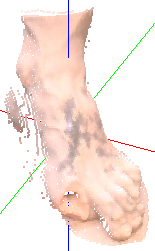
\includegraphics[width=0.5\textwidth]{ICP/prueba_ICP_2_1} 
		\caption*{Conjunto (1) con $ 7\,042 $ puntos.}
		%\label{fig:subim1}
	\end{minipage}
	\begin{minipage}[b]{0.5\textwidth}
		\centering
		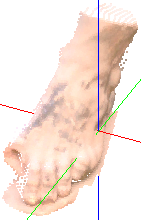
\includegraphics[width=0.5\textwidth]{ICP/prueba_ICP_2_2}
		\caption*{Conjunto (2) con $ 8\,334 $ puntos.}
		%\label{fig:subim2}
	\end{minipage}
	
	\caption{Tomas a alinear.}
	\label{fig:ICP_2}
\end{figure}

Tras la etapa de prealineado (los puntos seleccionados aparecen en la figura \ref{pre1}) se ha obtenido el resultado que muestran la figura \ref{pre2}. \\
\begin{figure}[h!]
	\begin{minipage}[b]{0.5\textwidth}
		\centering
		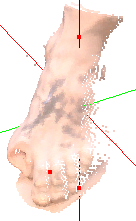
\includegraphics[width=0.5\textwidth]{ICP/prueba_ICP_2_3_1} 
		\caption*{Puntos clave del primer conjunto.}
		%\label{fig:subim1}
	\end{minipage}
	\begin{minipage}[b]{0.5\textwidth}
		\centering
		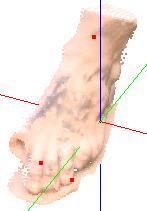
\includegraphics[width=0.5\textwidth]{ICP/prueba_ICP_2_3_2}
		\caption*{Puntos clave del segundo conjunto.}
		%\label{fig:subim2}
	\end{minipage}
	\caption{Etapa de prealineado.}
	\label{pre1}
\end{figure}
\begin{figure}[h!]
	
	\begin{minipage}[b]{0.5\textwidth}
		\centering
		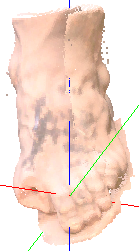
\includegraphics[width=0.5\textwidth]{ICP/prueba_ICP_2_3_3} 
		\caption*{Vista 1}
		%\label{fig:subim1}
	\end{minipage}
	\begin{minipage}[b]{0.5\textwidth}
		\centering
		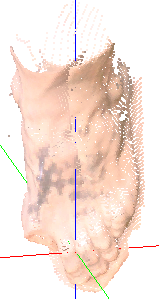
\includegraphics[width=0.5\textwidth]{ICP/prueba_ICP_2_3_4}
		\caption*{Vista 2}
		%\label{fig:subim2}
	\end{minipage}
	\caption{Vistas tras prealinear.}
		\label{pre2}
\end{figure}

A continuación, comenzamos usamos el algoritmo ICP. La tabla \ref{table:ICP2} recoge los datos tras cada iteración. Destacar que con distancia nos referimos a la distancia media entre los puntos y los más cercanos, es decir, lo que hemos notado como $ e_k $ y $ d_k $ en la sección \ref{algICP}. Por su parte, la figura \ref{fig:subim2}, muestra el resultado final tras las cinco iteraciones llevadas a cabo. \\

\begin{table}[h!]
	\centering
	\begin{tabular}{| c | c | c | c |} 
		\hline
		Iteración & Dist. antes (mm)  & Dist. después (mm) & Segundos \\
		\hline
		1 & 21.2000 & 18.1299 & 62.8672\\		 
		2 & 16.7174 &  15.8707 &  62.7888\\	
		3 & 15.1625 & 14.4617  & 62.8636\\
		4 & 13.9753 &  13.7418 & 63.059\\
		5 &  13.6518 &  13.6071 & 62.8259\\
		\hline
	\end{tabular}
	\caption{Resultados ajuste mediante ICP.}
	\label{table:ICP2}
\end{table}

\begin{figure}[h!]
	
	\begin{minipage}[b]{0.5\textwidth}
		\centering
		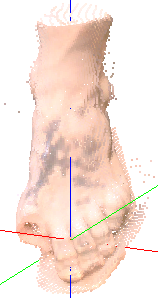
\includegraphics[width=0.5\textwidth]{ICP/prueba_ICP_2_3_5} 
		%\caption{Vista 1}
		%\label{fig:subim1}
	\end{minipage}
	\begin{minipage}[b]{0.5\textwidth}
		\centering
		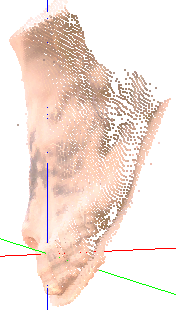
\includegraphics[width=0.5\textwidth]{ICP/prueba_ICP_2_3_6}
		%\caption{Vista 2}
	\end{minipage}
	\caption{Vistas tras cinco iteraciones del ICP.}
	\label{fig:subim2}
\end{figure}
En conclusión, vemos cómo el programa propuesto ha sido capaz de realizar un buen ajuste y por ello hemos conseguido un modelo más completo al original uniendo ambas tomas. Destacamos nuevamente la importancia que tiene en el proceso el prealineado. No solo la necesidad de hacerlo sino también la manera en la que sea lleva a cabo este proceso. Es posible que incluso incluyendo esta etapa el resultado no sea el deseado. Este comportamiento se debe como  ya hemos indicado a la convergencia local del método ICP. Las dos nubes de puntos tienen que estar los no solo lo suficientemente cerca sino también colocadas de tal manera que el algoritmo propuesto solo deba realizar un pequeño ajuste. \\

Por otro lado, también vemos que el tiempo empleado es elevado tal y como se indicó en la observación \ref{ObsTmp}: cada iteración ha durado algo más de un minuto. Hay que tener en cuenta que las nubes de puntos tomadas como modelo tienen un tamaño muy pequeño. En situaciones reales las tomas pueden tener millones de puntos lo que conllevaría mucho tiempo a la hora de aplicar el algoritmo e incluso sin la certeza de si el resultado es el que deseamos. En la siguiente sección planteamos unos métodos para acelerar este proceso.

%% \section{Aleatorios}

\chapter{Cambios en el método: uso de normales}
En las sección anterior nos encontramos con el siguiente problema: el método ICP funciona correctamente pero es demasiado lento ya que tiene un orden cuadrático y manejamos gran cantidad de información. Nuestro objetivo es entonces reducir el conjunto de puntos con los que trabajamos sin perder información. Este proceso no puede ser aleatorio y debe ser lo más significativo posible ya que, de lo contrario, podríamos obtener un resultado no deseado. Así usaremos en estos procedimientos los denominados \textit{descriptores}. Un descriptor lo podríamos definir como una medida de un punto en base a cierta característica que escojamos. De este modo obtenemos los llamados \textit{puntos significativos}, \textit{puntos clave} o \textit{key points} de cada una de las tomas. Como en nuestro marco de trabajo los modelos que tomamos como base son rígidos, es decir, no hay movimiento, cambios de escala, etc. podemos suponer que los puntos clave detectados en una toma deben de ser los mismos que en la otra. Por lo tanto, en una primera aproximación,  si realizamos el proceso para buscar la mejor transformación solo con los puntos clave deberíamos conseguir nuestro objetivo. \\

Como observación, aclarar que del mismo modo que no existe un método que funcione correctamente en el alineado de cualquier modelo, no existe un descriptor que funcione de manera adecuada con todos los modelos. Por ejemplo, podríamos detectar puntos clave en base al color. Si nos encontramos ante una escultura con un ropaje colorido y detallado es un descriptor que podríamos considerar válido. Sin embargo, si nuestro modelo presenta un color plano o una variación poco significativa del mismo no conseguiremos obtener puntos significativos. También debemos de tener en cuenta el tiempo necesario para la detección de puntos clave. El proceso debe ser lo suficientemente rápido para que reduzcamos el tiempo de alineación de las tomas y lo suficientemente bueno para que el conjunto de puntos calculado sea pequeño y descriptivo dentro de toda la nube.

\section{Variación de la normal}\label{varNormal}
El método para la obtención de puntos consistirá en la detección de zonas donde se produzca un cambio brusco de la normal calculando de este modo esquinas, hendiduras, etc.  Este procedimiento no es válido en superficies suaves ya que la variación de la normal en un entorno sería parecida en todo el modelo. Situación de este tipo nos la podemos encontrar, por ejemplo, en esferas. Una vez explicada la idea principal procedemos a explicar el proceso llevado a cabo. \\

En primer lugar, debemos calcular las normales de cada punto de la nube. Generalmente, es un proceso costoso aunque en nuestra  situación tenemos una gran ventaja. La información aportada por escáner con el que tomamos cada una de la muestras nos aporta, en cierta medida, una malla implícita ya que que puede entregar los datos de los puntos registrados siguiendo una cuadrícula en un archivo con formato PTX, que nos aporta el resultado por columnas por lo que podemos reconstruir la ``matriz'' espacial calculada previamente. Así con esta información para cada punto calculamos la normal mediante el producto vectorial de los triángulos adyacentes y luego promediamos obteniendo la de cada punto. En la figura \ref{Malla}, vemos a la izquierda la malla implícita que obtenemos con el formato que estamos trabajando. A la derecha aparece un ejemplo de cómo se han calculado las normales. En amarillo aparecen los vectores que se calculan (siempre y cuando existan dichos puntos) y en rojo los productos vectoriales necesarios. Destacamos que es importante que todas las normales tengan un convenio general de apuntar hacia dentro o hacia fuera del modelo. El nuestro ha sido de que apunten hacia afuera, lo que se ha tenido en cuenta durante la obtención de los productos vectoriales. \\

\begin{figure}[h!]
	
	\begin{minipage}{0.5\textwidth}
		\centering
		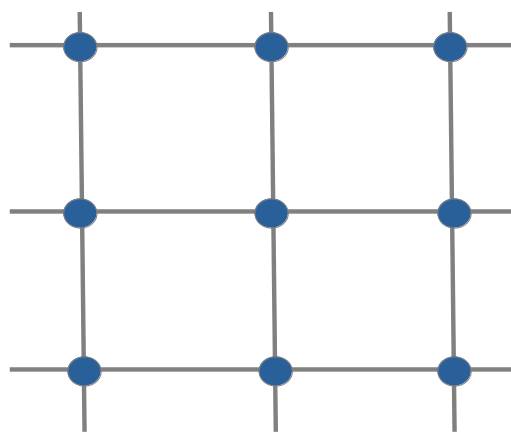
\includegraphics[width=0.65\linewidth, height=4cm]{Otros/Normal_1} 
		\caption*{(a)}
		%\label{fig:subim1}
	\end{minipage}
	\begin{minipage}{0.5\textwidth}
		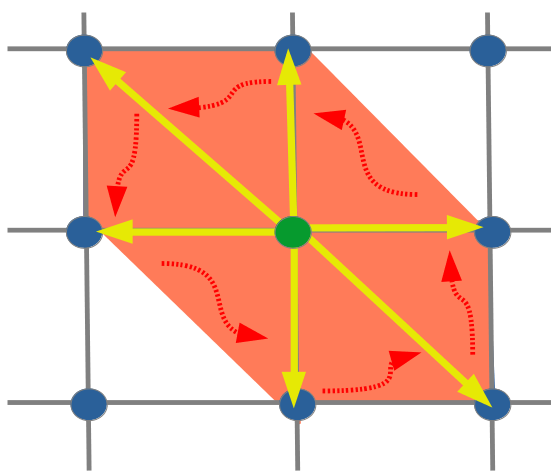
\includegraphics[width=0.8\linewidth, height=4cm]{Otros/Normal_2}
		\caption*{(b)}
		%\label{fig:subim2}
	\end{minipage}
	\caption{(a) Malla ímplicta, (b) Cálculo de la normal.}
	\label{Malla}
\end{figure}

La idea del algoritmo propuesto se basa en que en zonas relativamente planas las normales son muy parecidas por lo que la suma los productos escalares de la normal en un punto con aquellos contenidos en un entorno suyo es prácticamente 0. Razonemos lo que pasa en los lugares en los que hay esquinas. Tomamos un punto y sus vecinos, que en general son un total de 8. Suponemos una situación ideal en la que el punto que hemos escogido está en un borde. Si es así, consideramos que dos de los puntos adyacentes también están en dicho borde. \begin{comment}
INCLUIR DIBUJO !!!!!!!!!!!!!!!11
\end{comment} 
Así, tenemos que de sus vecinos adyacentes, dos tienen una normal parecida y los seis restantes perpendicular. Si calculamos el producto escalar medio en esta situación ideal obtenemos que es de $ 0.25 $. Por ello, el algoritmo propuesto tiene en cuenta este valor y solo se queda con los puntos cuyo descriptor de normales esté en un rango próximo al valor comentado, que pertenecería a la situación ideal. En nuestros experimentos hemos usado como criterio que el valor del producto escalar medio esté entre $ 0.15 $ y $ 0.3 $. \\

A continuación mostramos un ejemplo de los resultados obtenidos. Para ello, hemos usado diferentes niveles de precisión. Esto se ha conseguido simplificando la malla implícita que tenemos del modelo e indicando el número de filas y columnas que queremos conservar. Por ejemplo, si tenemos un nivel de precisión de 5, toma como puntos válidos aquellos que están cada 5 filas y 5 columnas. De este modo, de cada 25 puntos nos quedamos con uno. Si el nivel de precisión es 8, nos quedamos con un punto de 64. En la figura \ref{Ej_simpli} se muestran varios ejemplos de cómo varía la densidad de la malla en función del nivel de simplificado.
\begin{figure}[h!]
	\centering
	\begin{minipage}[b]{0.45\textwidth}
		\centering
		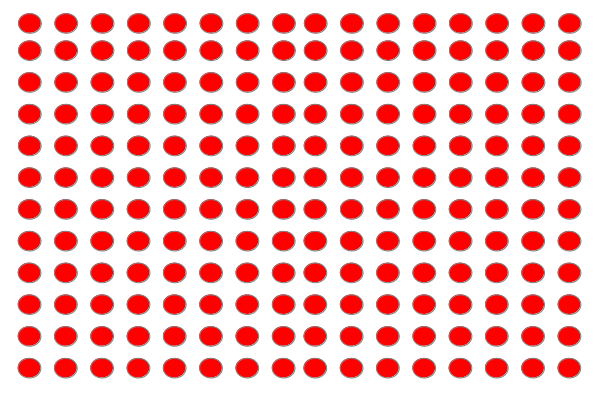
\includegraphics[width=0.7\textwidth]{Otros/Simp_0}
		\caption*{(a)}
	\end{minipage}
	\begin{minipage}[b]{0.45\textwidth}
		\centering
		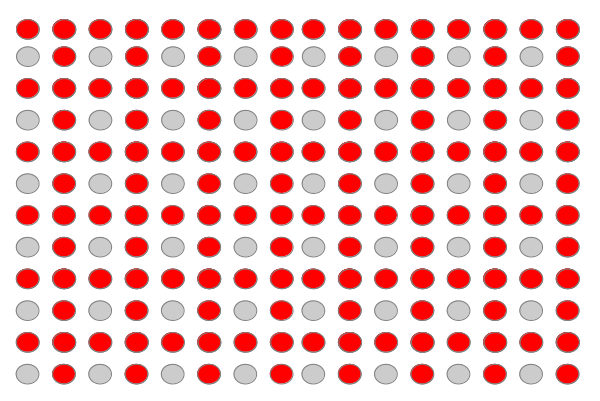
\includegraphics[width=0.7\textwidth]{Otros/Simp_2}
		\caption*{(b)}
	\end{minipage}
	\begin{minipage}[b]{0.45\textwidth}
		\centering
		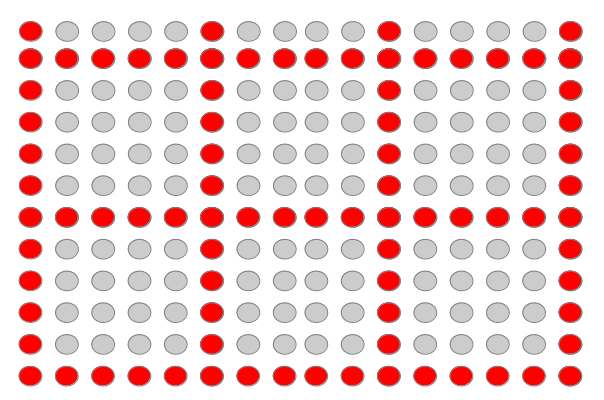
\includegraphics[width=0.7\textwidth]{Otros/Simp_5}
		\caption*{(c)}
	\end{minipage}
	\caption{Ejemplos de simplificado de la malla: (a) sin simplificado, (b) valor 2 y (c) valor 5. En rojo aparecen marcados los puntos con los que nos quedamos en cada caso.}
	\label{Ej_simpli}
\end{figure}

\begin{table}[h!]
	\centering
	\begin{tabular}{| c | c | c | c | c |} 
		\hline
		\thead{Nivel de\\ simplificado} & \thead{Puntos \\ totales}  & \thead{Tiempo cálculo \\normales (seg. )} & \thead{Tiempo cálculo \\ptos. clave (seg. )} & \thead{Puntos \\ clave} \\
		\hline
		1 & 2\,275\,886 & 25.1373 & 13.0592 & 592\,611 \\			 
		2 & 568\,830 & 6.39203  &  3.26905 & 192\,031 \\
		3 & 252\,881 & 2.82 &  1.47162 & 46\,610 \\
		4 &  142\,186 &  1.72909 &  0.837061 & 11\,866\\
		5 & 90\,983 & 1.00018 & 0.549648 & 4490 \\
		8 & 35\,519 &   0.394472 &   0.215125 &  1\,885\\
		\hline
	\end{tabular}
	\caption{Resultados del cálculo de puntos clave. En la primera columna aparece el nivel de simplificado utilizado, en la segunda el número total de puntos de la malla (simplificada), en la tercera y cuarta se incluye el tiempo en segundos para el cálculo de las normales y el cálculo de los valores del descriptor respectivamente. En la última columna se aporta el número de puntos clave obtenidos en cada caso. }
	\label{table:desNormales}
\end{table}

\begin{figure}[h!]
	\begin{minipage}[b]{0.5\textwidth}
		\centering
		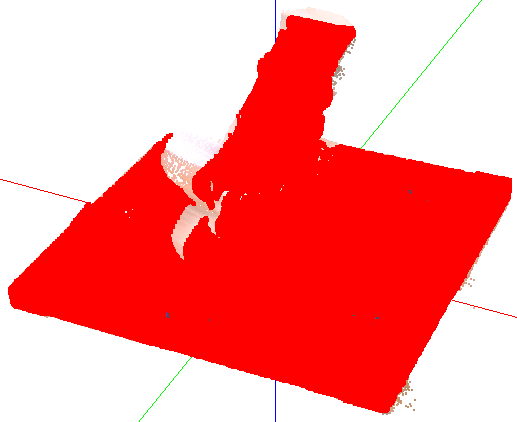
\includegraphics[width=0.7\textwidth]{ICP/desNormal-simp2}
		\caption*{Simplificado 2}
	\end{minipage}
	\begin{minipage}[b]{0.5\textwidth}
		\centering
		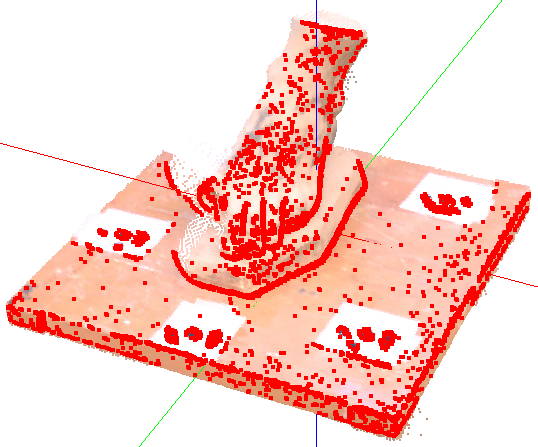
\includegraphics[width=0.7\textwidth]{ICP/desNormal-simp5}
		\caption*{Simplificado 5}
	\end{minipage}
	\begin{center}
		\begin{minipage}[b]{0.5\textwidth}
		\centering
		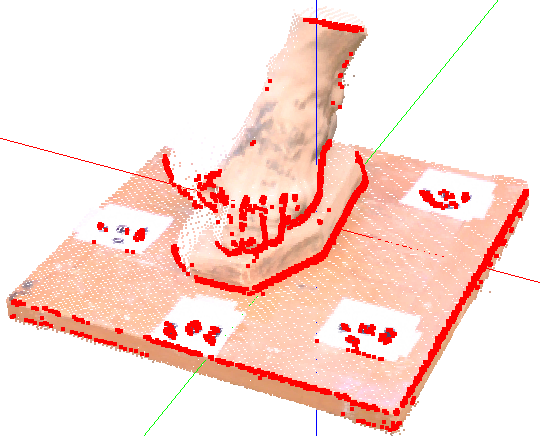
\includegraphics[width=0.7\textwidth]{ICP/desNormal-simp8}
		\caption*{Simplificado 8}
	\end{minipage}
	\end{center}
	\caption{Descriptor normales según el nivel de simplificado.}
	\label{Ej_simpli_real}
\end{figure}
Los resultados obtenidos tras aplicar el algoritmo de detección de puntos claves se muestran en la tabla \ref{table:desNormales} y figura \ref{Ej_simpli_real}. Vemos que uno de los problemas que tiene este método es que muy sensible al ruido. Cuanto más preciso sea el modelo base menos adecuado es el descriptor propuesto. Por lo tanto, si queremos que los puntos obtenidos tras el proceso sean significativos tenemos que calcularlos a partir del modelo simplificado. Esto no debe de ser una problema ya que esto solo lo usaremos en las primeras iteraciones del método ICP ya que para obtener la solución deseada debemos tener en cuenta posteriormente el modelo entero debido a la sensibilidad del procedimiento. 

\section{Pruebas}
\subsection{De puntos clave a todo el modelo}
La primera prueba que se va a realizar es aplicar el procedimiento a los puntos clave pero tomados de parte de una toma a una otra toma completa que tomamos como modelo. Lo explicamos con nuestro ejemplo base del pie. Si probamos con las mismas tomas de la sección \ref{ejemPrac1} en las que solo aparece el pie los puntos que nos aportará el descriptor mediante normales es posible que no tengan una correspondencia clara con la otra toma, sobre todo, los que se encuentran en el borde. Por eso, debemos tomar como modelo la toma completa para asegurar en todo lo que posible que haya correspondencia entre los puntos clave aportados. Del mismo modo, también habría problemas si tomamos las dos tomas completas ya que nuevamente es probable que algunos puntos no estén en el modelo, y al intentar ajustarlos, nos aporte una solución errónea. \begin{comment}
Sección sola de aproximaciones erróneas
\end{comment} 
Destacamos que aplicar el procedimiento propuesto a una parte de las tomas no debe de ser restrictivo porque nos interesa conocer la transformación. Podríamos almacenar los datos de las transformaciones que se van realizando y posteriormente aplicarlo a la toma completa. Otra solución sería, por ejemplo, imponer una distancia máxima entre dos puntos para asegurarse de que realmente se corresponden. Esta solución será la que usaremos en la siguiente sección.\\

\begin{figure}[h!]

	\begin{minipage}[b]{0.5\textwidth}
		\centering
		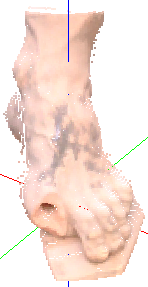
\includegraphics[width=0.3\linewidth]{ICP/prueba_ICP_3_1} 
		\caption*{Conjunto (1) con  7\,527 puntos.}
		%\label{fig:subim1}
	\end{minipage}
	\begin{minipage}[b]{0.5\textwidth}
		\centering
		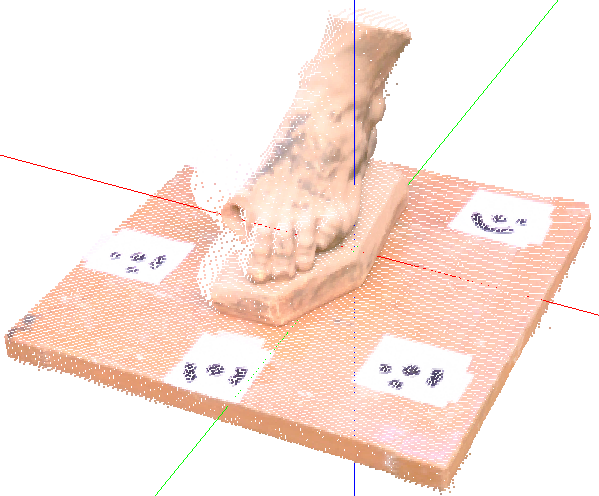
\includegraphics[width=0.6\linewidth]{ICP/prueba_ICP_3_2}
		\caption*{Conjunto (2) con 79\,921 puntos.}
		%\label{fig:subim2}
	\end{minipage}
	
	\caption{Tomas a alinear.}
\end{figure}

El número de puntos característicos detectados en la toma de la izquierda mediante el descriptor de las normales en el intervalo (0.15, 0.3) es de 506. Aplicamos el procedimiento y los resultados obtenidos se muestran en la figura \ref{clave1} y en la tabla \ref{table:ICPKPtotal}.\\

\begin{figure}[h!]
	\begin{minipage}[b]{0.5\textwidth}
		\centering
		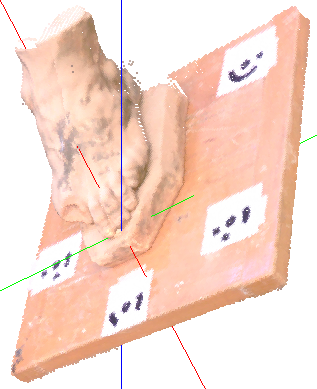
\includegraphics[width=0.65\linewidth]{ICP/prueba_ICP_3_3} 
		\caption*{Situación inicial.}
		%\label{fig:subim1}
	\end{minipage}
	\begin{minipage}[b]{0.5\textwidth}
		\centering
		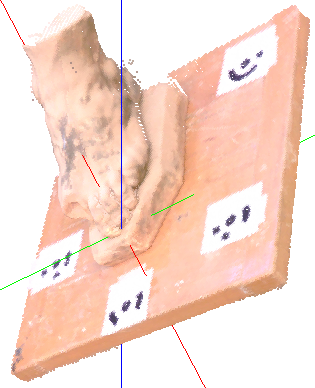
\includegraphics[width=0.65\linewidth]{ICP/prueba_ICP_3_4}
		\caption*{Resultado tras una iteración.}
		%\label{fig:subim2}
	\end{minipage}
	\begin{center}
		\begin{minipage}[b]{0.5\textwidth}
		\centering
		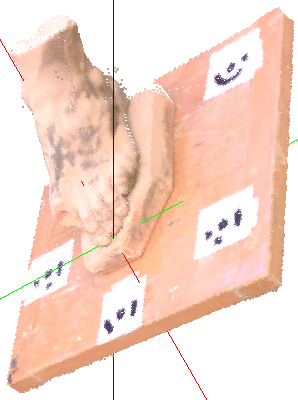
\includegraphics[width=0.65\linewidth]{ICP/prueba_ICP_3_5}
		\caption*{Resultado final.}
		%\label{fig:subim2}
	\end{minipage}
	\end{center}

	\caption{Algoritmo ICP usando un conjunto de puntos clave.}
	\label{clave1}
\end{figure}

\begin{table}[h!]
	\centering
	\begin{tabular}{| c | c | c | c |} 
		\hline
		Iteración & Dist. antes ($ m^2 $)  & Dist. después ($ m^2 $) & Segundos \\
		\hline
		1 &  0.000545768 &  0.00028771 & 20.0778\\			 
		2 & 0.000260278 & 0.000240228 &   19.7434\\	
		3 & 0.000231921 & 0.00022784  & 19.4636\\
		4 & 0.000224222 &  0.00022315 & 19.4807\\
		\hline
	\end{tabular}
	\caption{Resultados ajuste mediante ICP.}
	\label{table:ICPKPtotal}
\end{table}

Vemos que el procedimiento funciona correctamente y además que el tiempo empleado se reduce considerablemente respecto a los tiempos que habríamos necesitado considerando los conjuntos completos. Para hacernos una idea del tiempo que habría tardado basta tomar el ejemplo del pie de la sección \ref{ejemPrac1}. En ese caso, los conjuntos tenían unos 7\,000 y 8\,000 puntos cada uno y tardaba poco más de un minuto. Ahora unos de ellos tiene casi 80\,000, por lo que teniendo en cuenta el orden cuadrático del método, incrementaría bastante el tiempo necesario para completar cada iteración. Destacar que al igual que el procedimiento original, es posible que el resultado obtenido no sea el deseado y tenga que aplicarse desde el principio.
\subsection{De puntos clave a puntos clave}
Nuestro propósito ahora es intentar reducir aún más el conjunto de puntos con los que realizar el proceso ICP. Para ello, vamos a probar qué pasa si aplicamos el algoritmo solamente a los conjuntos de puntos clave calculados. Este paso hay que hacerlo con cuidado ya que, incluso en mayor medida que tomando en una muestra la toma entera, nos arriesgamos a que muchos puntos no tengan una correspondencia. Así, para el cálculo del punto más cercano se ha tenido en cuenta: 

\begin{enumerate}
\item Solo se comprueban puntos clave con un valor de descriptor parecido. Así, se ha fijado una diferencia máxima permitida y solo se comprueban los puntos que tengan un valor dentro de ese intervalo. Este se debe a que al ser movimientos rígidos no hay ningún tipo de deformación por lo que los planos serán los ``mismos'' mismos entre una toma y otra. Sin embargo, ponemos un intervalo debido a los errores del escáner y a las pérdidas de precisión debido al simplificado del modelo para la obtención de puntos clave.
\item Se ha acotado la distancia máxima permitida para un punto. Así, una vez calculada la distancia mínima de un punto al otro conjunto comprobamos que esa distancia no supere un umbral que hemos prefijado. Si lo supera significa que el punto más cercano está demasiado lejos y por ello no se corresponden realmente. De este modo, nos aseguramos que zonas que no se solapen se intenten ajustar y acabemos teniendo una solución errónea. 
\end{enumerate}

En la figura \ref{fig:KPKPICP} mostramos un ejemplo del resultado obtenido imponiendo que los valores de los descriptores entre los puntos claven difieran en $ 0.01 $ y que la distancia (en metros al cuadrado) entre ellos no sea mayor a $ 0.1 $. \\

\begin{figure}[h!]
	
	\begin{minipage}[b]{0.5\textwidth}
		\centering
		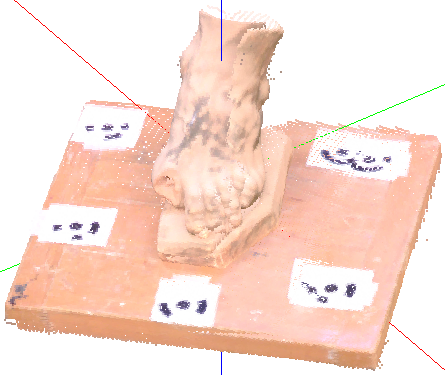
\includegraphics[width=0.9\linewidth]{ICP/prueba_ICP_4_1} 
		\caption*{Tras prealineado.}
		%\label{fig:subim1}
	\end{minipage}
	\begin{minipage}[b]{0.5\textwidth}
		\centering
		\includegraphics[width=0.9\linewidth]{ICP/prueba_ICP_4_2}
		\caption*{Tras dos iteraciones.}
		%\label{fig:subim2}
	\end{minipage}
	\caption{Proceso ICP solo con puntos clave.}
	\label{fig:KPKPICP}
\end{figure}

Se han realizado dos iteraciones. En ambas ha tardado aproximadamente $ 0.7 $ segundos y la distancia media (en metros al cuadrado) ha variado de $ 0.000782562 $ a $ 0.000722275 $. Los puntos clave calculados en cada caso son en el primera toma un total de $ 1142 $ y en la segunda $ 2273 $. Observamos cómo tras las dos iteraciones se han conseguido ajustar mejor las dos tomas. Nuevamente, hacemos hincapié en que el algoritmo ha tardado menos de lo que habría necesitado en caso de haber tomado las nubes de puntos completas gracias a la reducción del número de elementos de ambos conjuntos. \\

Una segunda aproximación es contar el número de productos escalares que dan ``cero'' para saber el número de planos perpendiculares que tiene cada punto. De este modo, solo comparamos con puntos cuyo número de ceros es el mismo. Se ha tomado perpendicularidad cuando el producto escalar sea menor que $ 0.01 $ debido a errores en la toma de muestras y simplificado de la malla. Notar que seguimos teniendo en cuenta la cota de la distancia máxima. Esto puede hacer que en un paso del método la distancia puede ser mayor que el anterior al existir un mayor o menor número de puntos que se han tomado como referencia. Esto no debería ser ningún problema \textit{a priori}. En el ejemplo que mostramos ese número no ha variado entre iteraciones.

\begin{table}[h!]
	\centering
	\begin{tabular}{| c | c | c | c |} 
		\hline
		Iteración & Dist. antes ($ m^2 $)  & Dist. después ($ m^2 $) & Segundos \\
		\hline
		1 &  0.00124479 &  0.00121367 & 2.33132\\			 
		2 & 0.00119796 &  0.0011896 &   2.32062\\	
		3 &  0.00118431 & 0.00118055  & 2.30985\\
		4 & 0.00117839 &  0.00117688 & 2.32283\\
		\hline
	\end{tabular}
	\caption{Resultados ajuste mediante ICP.}
\end{table}

\begin{figure}[th!]
	
	\begin{minipage}[b]{0.5\textwidth}
		\centering
		\includegraphics[width=0.9\linewidth]{ICP/prueba_ICP_5_1} 
		\caption*{Tras prealineado.}
		%\label{fig:subim1}
	\end{minipage}
	\begin{minipage}[b]{0.5\textwidth}
		\centering
		\includegraphics[width=0.95\linewidth]{ICP/prueba_ICP_5_2}
		\caption*{Tras cuatro iteraciones.}
		
		%\label{fig:subim2}
	\end{minipage}
	
	\caption{Proceso ICP solo con puntos clave agrupándolos por el número de ceros de sus productos escalares.}
	\label{fig:ICPej5}
\end{figure}

En la figura \ref{fig:ICPej5}, vemos que nuevamente se ha obtenido un proceso satisfactorio en la zona de los dedos del pie aunque ha tardado más tiempo en cada iteración que en el caso anterior.
\input{capitulos/Más-ejemplos.tex}

\chapter{RANSAC: algoritmo de consenso}
En esta sección estudiaremos otro de los algoritmos más utilizados para la alineación de dos nubes de puntos. Se trata del algoritmo \textit{Random Sample Consensus} (RANSAC). El método ICP que acabamos de ver podríamos decir que es específico para la solución de nuestro problema, es decir, no se utiliza más allá de la situación en la que lo hemos estudiado. Por su parte, el algoritmo RANSAC es más genérico y utilizado en otras tareas diferentes. Su finalidad es la de ajustar parámetros de un modelo matemático que viene determinado por un conjunto de observaciones. Nosotros lo utilizaremos para la detección de superficies planas en nuestros modelos que a su vez las utilizaremos para la obtención de sus puntos intersección. Esos puntos que podríamos considerarlos como clave, siguiendo la nomenclatura utilizada, serán la base para el alineado. Destacar que es considerado un algoritmo robusto incluso bajo la existencia de gran cantidad de valores atípicos y que sigue un paradigma de hipótesis-y-prueba.

\section{Algoritmo}
Este algoritmo fue propuesto por A. Fischler y Robert C. Bolles en \cite{fischler1981random}. Este será el artículo que seguiremos como referencia en lo que respecta a la explicación matemática de la veracidad del método. Como hemos dicho en la introducción, podemos considerar que es un algoritmo del tipo hipótesis-y-prueba. A diferencia de otros algoritmos, no tiene en cuenta todo el conjunto, sino que toma el menor número posible de puntos necesarios para ajustar el modelo y comprueba si efectivamente esos puntos determinan el modelo que queremos. En nuestro caso, el modelo que deseamos obtener es un plano.\\

El algoritmo consta de las siguientes etapas:
\begin{enumerate}
\item Tomar de manera aleatoria el mínimo número de puntos necesarios que define el modelo.
\item Con una tolerancia $ \varepsilon$, contar el número de puntos que distan del modelo definido en el punto anterior.
\item Repetir 1 y 2 un total de $ N $ veces y quedarse con el que contenga una mayor cantidad de puntos.
\end{enumerate}

De este modo, podemos considerar que el algoritmo necesita, por ahora, tres parámetros. El primero de ellos, el mínimo número de puntos para definir el modelo. Por ejemplo, si queremos obtener una recta debemos tomar 2 puntos mientras que si queremos obtener un plano debemos coger 3. También tenemos que decidir una tolerancia $ \varepsilon $ que depende, en cierto modo, de la nube de puntos que tenemos entre manos y del resultado final que queremos. Finalmente, hay que decidir un $ N $ que determina el número de veces que repetimos el proceso. Su cálculo se explicará en siguientes secciones pero destacamos ahora que debe de ser lo suficientemente grande para asegurar que este proceso aleatorio conseguirá nuestro objetivo. \\

Antes de continuar, veamos un ejemplo sencillo en dos dimensiones donde explicaremos cómo funciona este procedimiento. Supongamos que tenemos la nube de la figura \ref{fig:ejransac0}. \\

\begin{figure}[h!]
	\centering
	\includegraphics[width=0.5\linewidth]{imagenes/Ej-RANSAC/ejRANSAC_0}
	\caption{Nube de puntos.}
	\label{fig:ejransac0}
\end{figure}

Queremos aplicarle el algoritmo RANSAC para obtener una recta dentro de ella. Para ello, primero cogemos dos puntos aleatorios del modelo, calculamos la recta que pasa por ellos, y obtenemos los puntos que distan de la misma una distancia menor que $ \varepsilon $. Supongamos que la situación es la que se muestra en la figura \ref{fig:RNASAC-s1}. \\

\begin{figure}[h!]
	\begin{minipage}[b]{0.5\textwidth}
		\centering
		%\includegraphics[width=1\linewidth]{Buyer_call} 
		\includegraphics[width=1\linewidth]{Ej-RANSAC/ejRANSAC_10} 
		\caption*{Selección de puntos.}
		%\label{fig:subim1}
	\end{minipage}
\begin{minipage}[b]{0.5\textwidth}
	\centering
	%\includegraphics[width=1\linewidth]{Buyer_call} 
	\includegraphics[width=1\linewidth]{Ej-RANSAC/ejRANSAC_11} 
	\caption*{Construcción de la recta}
	%\label{fig:subim1}
\end{minipage}
\begin{center}
	\begin{minipage}[b]{0.5\textwidth}
	\centering
	%\includegraphics[width=1\linewidth]{Buyer_call} 
	\includegraphics[width=1\linewidth]{Ej-RANSAC/ejRANSAC_12} 
	\caption*{Vemos la bondad del modelo.}
	%\label{fig:subim1}
\end{minipage}
\end{center}
	\caption{Primer paso del algoritmo RANSAC.}
	\label{fig:RNASAC-s1}
\end{figure}

Si contamos el número de puntos que se ajustan al modelo, vemos que hay un total de 8. Repetimos el proceso y, en una iteración determinada, se obtiene el modelo de la figura \ref{fig:RNASAC-s2}.\\

\begin{figure}[h!]
	\begin{minipage}[b]{0.5\textwidth}
		\centering
		%\includegraphics[width=1\linewidth]{Buyer_call} 
		\includegraphics[width=1\linewidth]{Ej-RANSAC/ejRANSAC_20} 
		\caption*{Selección de puntos.}
		%\label{fig:subim1}
	\end{minipage}
	\begin{minipage}[b]{0.5\textwidth}
		\centering
		%\includegraphics[width=1\linewidth]{Buyer_call} 
		\includegraphics[width=1\linewidth]{Ej-RANSAC/ejRANSAC_21} 
		\caption*{Construcción de la recta}
		%\label{fig:subim1}
	\end{minipage}
	\begin{center}
		\begin{minipage}[b]{0.5\textwidth}
		\centering
		%\includegraphics[width=1\linewidth]{Buyer_call} 
		\includegraphics[width=1\linewidth]{Ej-RANSAC/ejRANSAC_22} 
		\caption*{Vemos la bondad del modelo.}
		%\label{fig:subim1}
	\end{minipage}
	\end{center}
	\caption{Paso del algoritmo RANSAC.}
	\label{fig:RNASAC-s2}
\end{figure}
Ene esta ocasión, un total de 27 puntos se ajustan al modelo. Si no se detectara en el resto de iteraciones un ajuste mejor, este sería el modelo que nos devolvería al algoritmo. \\

\section{Número de iteraciones}
Uno de los puntos clave del algoritmo es asegurarse de que el número de iteraciones $ N $ sea lo suficientemente grande para obtener puntos que ajusten correctamente el modelo que queremos. De este modo, sea $ p $ la probabilidad que al menos uno de los conjuntos tomados no contiene valores atípicos y $ 1-p $ de que todos los conjuntos contienen al menos un valor atípico. Notamos por $ u $, a la probabilidad de que un valor sea correcto y, por lo tanto, $ v = 1 - u $ es la probabilidad de ser un valor atípico. Sea $ m $ el número de puntos mínimo para definir el modelo: dos para una recta, tres para un plano, $ \dots $. Así, la probabilidad de escoger todos los puntos correctos en una iteración es $ u^m $ y la de escoger alguno incorrecto es $ 1-u^m $. Si hacemos un total de $ N $ iteraciones, la probabilidad de escoger siempre un valor atípico es $ (1-u^m)^N $. Pero esto no es más que
\[
1-p = (1-u^m)^N.
\]
Si despejamos el valor de $ N $,
\begin{equation}
N = \frac{\log(1-p)}{\log(1-u^m)} = \frac{\log(1-p)}{\log(1-(1-v)^m)}.
\end{equation}
El valor obtenido no tiene que ser obligatoriamente un número natural por lo que se toma el primero entero que supere o iguale dicho valor. La probabilidad $ p $ es entrada del algoritmo y debe ser elevado. También $ u $ (o $ v $) son parámetros que se eligen y que dependerán en cierto modo, del modelo con el que se está trabajando. La tabla \ref{table:RANSAcvalues} recoge diferentes valores de $ N $ en función de $ p $, $ v $ y $ m $.
% Please add the following required packages to your document preamble:
% \usepackage{multirow}
% Please add the following required packages to your document preamble:
% \usepackage{multirow}
% Please add the following required packages to your document preamble:
% \usepackage{multirow}
% Please add the following required packages to your document preamble:
% \usepackage{multirow}
% Please add the following required packages to your document preamble:
% \usepackage{multirow}
\begin{table}[]
	\centering
	\begin{tabular}{l|l|c|c|c|c|}
		\cline{2-6}
		& \multirow{2}{*}{$ m $} & \multicolumn{4}{c|}{$ v $}                                                                                     \\ \cline{3-6} 
		&                    & \multicolumn{1}{l|}{0.05} & \multicolumn{1}{l|}{0.2} & \multicolumn{1}{l|}{0.5} & \multicolumn{1}{l|}{0.8} \\ \hline
		\multicolumn{1}{|l|}{\multirow{2}{*}{$ p = $0.99 }} & 2                  & 2                         & 5                        & 17                       & 113                      \\ \cline{2-6} 
		\multicolumn{1}{|l|}{}                          & 3                  & 3                         & 7                        & 35                       & 574                      \\ \hline
		\multicolumn{1}{|l|}{\multirow{2}{*}{$ p = $0.9 }}  & 2                  & 1                         & 3                        & 9                        & 57                       \\ \cline{2-6} 
		\multicolumn{1}{|l|}{}                          & 3                  & 2                         & 4                        & 18                       & 287                      \\ \hline
		\multicolumn{1}{|l|}{\multirow{2}{*}{$ p = $0.8 }}  & 2                  & 1                         & 2                        & 6                        & 40                       \\ \cline{2-6} 
		\multicolumn{1}{|l|}{}                          & 3                  & 1                         & 3                        & 13                       & 201                      \\ \hline
	\end{tabular}
\caption{Número de iteraciones para diferentes valores de $ p $ (probabilidad), $ m $ (número de puntos para definir el modelo: 2 recta y 3 plano) y $ v $ probabilidad de ser un valor atípico.}
\label{table:RANSAcvalues}
\end{table}


\section{Ejemplos sencillos}
En esta sección, veremos cómo actúa al algoritmo en dos ejemplos concretos: el del pie y en el de la torre. En ambos casos usaremos los modelos simplificados tal y como hemos visto en la sección \ref{varNormal}. Esto no debería de ser una restricción, ya que la densidad total del modelo no varía y los planos se mantienen. Para cada, utilizaremos diferente valores de los parámetros y veremos cómo de buenos son los resultados obtenidos. Al ser modelos en los que buscamos planos el valor de $ m $ es 3. Destacamos que para el cálculo de la distancia entre el modelo y cada punto se ha hecho mediante la función distancia con signo (en valor absoluto).

\subsection{Pie}
Se ha tomado como nivel de tolerancia $ \varepsilon = 0.05 $, ya que ese valor depende sobre todo del modelo que estamos trabajando. El modelo consta de un total de $ 34.120 $ puntos. En la tabla \ref{table:RANSACpieTable} y en la figura \ref{fig:RANSACpie} están los resultados que nos proporciona. \\

\begin{figure}[h!]
	\begin{minipage}[b]{0.5\textwidth}
		\centering
		%\includegraphics[width=1\linewidth]{Buyer_call} 
		\includegraphics[width=0.8\linewidth]{Ej-RANSAC/pie_0-5_0-4} 
		\caption*{(a)}
		%\label{fig:subim1}
	\end{minipage}
	\begin{minipage}[b]{0.5\textwidth}
		\centering
		%\includegraphics[width=1\linewidth]{Buyer_call} 
		\includegraphics[width=0.8\linewidth]{Ej-RANSAC/pie_0-5_0-3} 
		\caption*{(b)}
		%\label{fig:subim1}
	\end{minipage}
	\begin{minipage}[b]{0.5\textwidth}
		\centering
		%\includegraphics[width=1\linewidth]{Buyer_call} 
		\includegraphics[width=0.8\linewidth]{Ej-RANSAC/pie_0-7_0-3} 
		\caption*{(c)}
		%\label{fig:subim1}
	\end{minipage}
	\begin{minipage}[b]{0.5\textwidth}
		\centering
		%\includegraphics[width=1\linewidth]{Buyer_call} 
		\includegraphics[width=0.8\linewidth]{Ej-RANSAC/pie_0-9_0-3} 
		\caption*{(d)}
		%\label{fig:subim1}
	\end{minipage}		
	\begin{minipage}[b]{0.5\textwidth}
		\centering
		%\includegraphics[width=1\linewidth]{Buyer_call} 
		\includegraphics[width=0.8\linewidth]{Ej-RANSAC/pie_0-9_0-5} 
		\caption*{(e)}
		%\label{fig:subim1}
	\end{minipage}
	\begin{minipage}[b]{0.5\textwidth}
		\centering
		%\includegraphics[width=1\linewidth]{Buyer_call} 
		\includegraphics[width=0.8\linewidth]{Ej-RANSAC/pie_0-9_0-7} 
		\caption*{(f)}
		%\label{fig:subim1}
	\end{minipage}	
	
	\caption{Resultados de aplicar RANSAC en el ejemplo del pie para diferentes parámetros (ver tabla \ref{table:RANSACpieTable}). }
	\label{fig:RANSACpie}
\end{figure}

\begin{table}[h!]
	\centering
	\begin{tabular}{| c | c | c || c | c |} 
		\hline
		Prueba & $ p $ & $ v $ & Tiempo (seg.) & Iteraciones \\
		\hline
		(a) & 0.5 & 0.4 & 0.052172 & 3 \\		
		(b) & 0.5 & 0.3 & 0.026094 & 2  \\	
		(c) & 0.7 & 0.3 & 0.055964 &  3 \\
		(d) & 0.9 & 0.3 & 0.116656 & 6\\
		(e) & 0.9 & 0.5 & 0.356769 & 18\\
		(f) & 0.9 & 0.7 & 1.712500 & 85\\
		\hline
	\end{tabular}
	\caption{Resultados de aplicar el algoritmo RANSAC una vez a una toma del pie. La primera columna identifica la prueba (ver figura \ref{fig:RANSACpie}), la segunda y tercera los valores de $ p $ y $ v $ escogidos y las dos últimas el tiempo empleado en el cálculo del plano y las iteraciones que se han realizado.}
	\label{table:RANSACpieTable}
\end{table}

Vemos que al ser un proceso aleatorio los resultados que se han obtenido son dispares pero en este caso, en un número ``bajo'' de iteraciones hemos visto que es capaz de detectar el plano que contiene el modelo.

\subsection{Torre}
Realizamos diferentes pruebas con nuestro modelo de la torre que consta de $ 431\,254 $ puntos. En esta ocasión se ha optado por una tolerancia de $ \varepsilon = 0.03 $. Los resultados se recogen en la tabla \ref{table:RANSACtorreTable} y en la figura \ref{fig:RANSACtorre}. \\

\begin{figure}[h!]
	\begin{minipage}[b]{0.5\textwidth}
		\centering
		%\includegraphics[width=1\linewidth]{Buyer_call} 
		\includegraphics[width=0.8\linewidth]{Ej-RANSAC/torre_0-5_0-4} 
		\caption*{(a2)}
		%\label{fig:subim1}
	\end{minipage}
	\begin{minipage}[b]{0.5\textwidth}
		\centering
		%\includegraphics[width=1\linewidth]{Buyer_call} 
		\includegraphics[width=0.8\linewidth]{Ej-RANSAC/torre_0-7_0-4} 
		\caption*{(b2)}
		%\label{fig:subim1}
	\end{minipage}
	\begin{minipage}[b]{0.5\textwidth}
		\centering
		%\includegraphics[width=1\linewidth]{Buyer_call} 
		\includegraphics[width=0.8\linewidth]{Ej-RANSAC/torre_0-7_0-6} 
		\caption*{(c2)}
		%\label{fig:subim1}
	\end{minipage}
	\begin{minipage}[b]{0.5\textwidth}
		\centering
		%\includegraphics[width=1\linewidth]{Buyer_call} 
		\includegraphics[width=0.8\linewidth]{Ej-RANSAC/torre_0-8_0-6} 
		\caption*{(d2)}
		%\label{fig:subim1}
	\end{minipage}		
	\begin{minipage}[b]{0.5\textwidth}
		\centering
		%\includegraphics[width=1\linewidth]{Buyer_call} 
		\includegraphics[width=0.8\linewidth]{Ej-RANSAC/torre_0-8_0-7} 
		\caption*{(e2)}
		%\label{fig:subim1}
	\end{minipage}
	\begin{minipage}[b]{0.5\textwidth}
		\centering
		%\includegraphics[width=1\linewidth]{Buyer_call} 
		\includegraphics[width=0.8\linewidth]{Ej-RANSAC/torre_0-85_0-8} 
		\caption*{(f2)}
		%\label{fig:subim1}
	\end{minipage}	
	
	\caption{Resultados de aplicar RANSAC en el ejemplo de la torre para diferentes parámetros (ver tabla \ref{table:RANSACtorreTable}). }
	\label{fig:RANSACtorre}
\end{figure}

\begin{table}[h!]
	\centering
	\begin{tabular}{| c | c | c || c | c |} 
		\hline
		Prueba & $ p $ & $ v $ & Tiempo (seg.) & Iteraciones \\
		\hline
		(a2) & 0.5 & 0.4 & 0.484033 & 3 \\		
		(b2) & 0.7 & 0.4 & 0.961606 & 5  \\	
		(c2) & 0.7 & 0.6 & 4.271831 &  19 \\
		(d2) & 0.8 & 0.6 & 5.749162 & 25\\
		(e2) & 0.8 & 0.7 & 14.00424 & 59 \\
		(f2) & 0.85 & 0.8 & 55.98620 & 237\\
		\hline
	\end{tabular}
	\caption{Resultados de aplicar el algoritmo RANSAC una vez a una toma de  la torre. La primera columna identifica la prueba (ver figura \ref{fig:RANSACpie}), la segunda y tercera los valores de $ p $ y $ v $ escogidos y las dos últimas el tiempo empleado en el cálculo del plano y las iteraciones que se han realizado.}
	\label{table:RANSACtorreTable}
\end{table}

Vemos que nuevamente se han podido obtener resultados buenos en relativamente pocas iteraciones.

\section{Cálculo de los puntos de intersección}
En esta sección, vamos a obtener mediante el algoritmo RANSAC un punto que sea intersección de tres planos. Para ello, tomamos el ejemplo de la torre. En primer lugar, veamos cómo calculamos dicha intersección. Lo único que tenemos que hacer, dado un conjunto de puntos que hemos obtenido como plano, es tomar una normal del mismo. Esta normal puede ser, por ejemplo, la misma que hemos usado para el cálculo de las distancias mediante la función distancia con signo que la podemos ir almacenando para evitar su cálculo posterior. Notamos a la normal obtenida para el paso $ i $ como $ N_i = (N_{i1}, N_{i2}, N_{i3}) \in \RR^3$. De este modo, cada punto $ (x,y,z) $ del conjunto debe cumplir la ecuación:
\[
N_{i1} x + N_{i2} y + N_{i3} z = d_i.
\]
Finalmente, solo nos queda calcular $ d _i$, que se puede hacer de manera sencilla sustituyendo el valor de $ (x,y,z) $ por un punto conocido del conjunto obtenido. Hemos calculado la ecuación del plano de una manera sencilla. Ahora solo nos queda calcular la intersección de tres planos. Para ello, tenemos que resolver el sistema para las iteraciones $ i,j,k $:

\[
\left.
\begin{array}{rcl}
&N_{i1}x + N_{i2}y + N_{i3}z  &= d_i \\ 
&N_{j1}x + N_{j2}y + N_{j3}z  &= d_j \\
&N_{k1}x + N_{k2}y + N_{k3}z  &= d_k
\end{array}
\right\}
\]
\[
\big\Updownarrow
\]
\[
\begin{pmatrix}
N_{i1} & N_{i2} & N_{i3}\\
N_{j1} & N_{j2} & N_{j3}\\
N_{k1} & N_{k2} & N_{k3}\\
\end{pmatrix}
\begin{pmatrix}
x\\
y\\
z\\
\end{pmatrix}
=
\begin{pmatrix}
d_i\\
d_j\\
d_k\\
\end{pmatrix}
\]
\[
\big\Updownarrow
\]
\[
A \begin{pmatrix}
x\\
y\\
z\\
\end{pmatrix}
=
\mathit{\mathbf{d}}.
\]

Si el sistema es compatible determinado, lo que significa que la intersección está formada solo por un punto, podemos calcular $ A^{-1} $ y obtenemos el punto de intersección como:
\[
\begin{pmatrix}
x\\
y\\
z\\
\end{pmatrix} = A^{-1}\mathbf{d}.
\]

Veamos este caso en el modelo real. Primero, obtenemos tres planos de la nube de puntos. Usamos el algoritmo con valor $ p = 0.8 $, $ v = 0.8 $ y $ \varepsilon = 0.03 $. Los planos que se han obtenido se muestran en la siguiente figura \ref{fig:RNASACptoInter}. \\
\begin{figure}[h!]
	\begin{minipage}{0.5\textwidth}
		\centering
		%\includegraphics[width=1\linewidth]{Buyer_call} 
		\includegraphics[width=0.8\linewidth]{Ej-RANSAC/torre_1-1} 
		%\label{fig:subim1}
	\end{minipage}
	\begin{minipage}{0.5\textwidth}
		\centering
		%\includegraphics[width=1\linewidth]{Buyer_call} 
		\includegraphics[width=0.8\linewidth]{Ej-RANSAC/torre_1-2} 
		%\label{fig:subim1}
	\end{minipage}
	\begin{center}
		\begin{minipage}{0.5\textwidth}
		\centering
		%\includegraphics[width=1\linewidth]{Buyer_call} 
		\includegraphics[width=0.8\linewidth]{Ej-RANSAC/torre_1-3} 
		%\label{fig:subim1}
	\end{minipage}
	\end{center}
	\caption{Planos detectados iterativamente en el ejemplo de la torre de las gallinas de la Alhambra. Los parámetros son $ p = 0.8 $, $ v = 0.8 $ y $ \varepsilon = 0.03 $.}
	\label{fig:RNASACptoInter}
\end{figure}

Los valores que se han obtenido han sido los siguientes:
\begin{itemize}
\item $ N_1 = ( \text{0.987981}, \text{ 0.154204}, \text{ 0.0107157}) $, $ d_1 = \text{ -0.50992} $.
\item $ N_2 = ( \text{-0.0192558}, \text{ 0.0458887}, \text{ 0.998761}) $, $ d_2 = \text{-1.13957} $.
\item $ N_3 = ( \text{0.147295}, \text{ -0.987795}, \text{ 0.0506549}) $, $ d_3 = \text{-1.34888}$.
\end{itemize}
Claramente, el sistema que forman es compatible determinado. Si lo resolvemos tal y como se ha explicado anteriormente obtenemos el punto cuyas coordenadas son (-0.690391, 1.20058, -1.20946), que se corresponde con el marcado en la figura \ref{fig:torre1-4}.
\begin{figure}
	\centering
	\includegraphics[width=0.4\linewidth]{imagenes/Ej-RANSAC/torre_1-4}
	\caption{Punto de intersección.}
	\label{fig:torre1-4}
\end{figure}


\section{Ejemplo despacho}
El objetivo de esta sección es probar el comportamiento del algoritmo en un ejemplo más complejo y del que podemos obtener un mayor número de planos. En concreto, se trata de dos tomas de un despacho. Destacamos que nuevamente se ha realizado el proceso de simplificado de las mismas con un nivel de 4 y tras este proceso se han obtenido aproximadamente $ 650\,000 $ puntos en cada toma. En la figura \ref{fig:tomasLab} se muestran ambas nubes de puntos. \\

\begin{figure}[h!]
	\begin{minipage}[b]{0.5\textwidth}
		\centering
		%\includegraphics[width=1\linewidth]{Buyer_call} 
		\includegraphics[width=1\linewidth]{lab/LAB0} 
		\caption*{Toma 0.}
		%\label{fig:subim1}
	\end{minipage}
	\begin{minipage}[b]{0.5\textwidth}
		\centering
		%\includegraphics[width=1\linewidth]{Buyer_call} 
		\includegraphics[width=0.8\linewidth]{lab/LAB1} 
		\caption*{Toma 1.}
		%\label{fig:subim1}
	\end{minipage}
	\caption{Tomas del laboratorio.}
	\label{fig:tomasLab}
\end{figure}

En primer lugar, veamos los planos que se obtienen al ejecutar el algoritmo RANSAC en la primera de ellas. Los planos obtenidos se muestran en la figura \ref{fig:planos-lab0}. Posteriormente, en la tabla \ref{table:res-lab0} aparece el tiempo empleado y el número de puntos detectados en cada plano. Finalmente, en la figura \ref{fig:inter0} están los puntos de intersección obtenidos. \\

\begin{figure}[h!]
	\centering
	\begin{minipage}{0.4\textwidth}
		\centering
		%\includegraphics[width=1\linewidth]{Buyer_call} 
		\includegraphics[width=1\linewidth]{lab/lab0-1} 
		%\label{fig:subim1}
	\end{minipage}
	\centering
	\begin{minipage}{0.4\textwidth}
		\centering
		%\includegraphics[width=1\linewidth]{Buyer_call} 
		\includegraphics[width=1\linewidth]{lab/lab0-2} 
		%\label{fig:subim1}
	\end{minipage}
	\begin{minipage}{0.4\textwidth}
		\centering
		%\includegraphics[width=1\linewidth]{Buyer_call} 
		\includegraphics[width=1\linewidth]{lab/lab0-3} 
		%\label{fig:subim1}
	\end{minipage}
	\centering
	\begin{minipage}{0.4\textwidth}
		\centering
		%\includegraphics[width=1\linewidth]{Buyer_call} 
		\includegraphics[width=1\linewidth]{lab/lab0-4} 
		%\label{fig:subim1}
	\end{minipage}
	\begin{minipage}{0.4\textwidth}
		\centering
		%\includegraphics[width=1\linewidth]{Buyer_call} 
		\includegraphics[width=1\linewidth]{lab/lab0-5} 
		%\label{fig:subim1}
	\end{minipage}
	\centering
	\begin{minipage}{0.4\textwidth}
		\centering
		%\includegraphics[width=1\linewidth]{Buyer_call} 
		\includegraphics[width=1\linewidth]{lab/lab0-6} 
		%\label{fig:subim1}
	\end{minipage}
	\caption{De izquierda a derecha y de arriba a abajo los planos que se han ido detectando en la toma 0.}
	\label{fig:planos-lab0}
\end{figure}

\begin{table}[h!]
	\centering
	\begin{tabular}{| c | c | c | c | c |} 
		\hline
		Iteración  & Tiempo (seg.) & Num. puntos \\
		\hline
		1 & 273.455 & 239\,099 \\				  
		2 & 169.570 & 98\,342  \\	
		3 & 113.872 &  27\,342 \\
		4 & 100.320 &   56\,325\\
		5 & 72.0483 & 46\,067 \\
		6 & 64.7628 & 17\,130 \\
		\hline
	\end{tabular}
	\caption{Resultados de aplicar RANSAC en la toma 0 del laboratorio. En la primera columna aparece el número de la iteración, en la segunda el tiempo empleado en segundos y en la tercera el número de puntos que contiene cada plano detectado.}
	\label{table:res-lab0}
\end{table}

\begin{figure}[h!]
		\centering
		%\includegraphics[width=1\linewidth]{Buyer_call} 
		\includegraphics[width=0.6\linewidth]{lab/inter0-pared+mesas} 
		\caption{Intersecciones entre los planos en la toma 0.}
		\label{fig:inter0}
\end{figure}

Repitamos el proceso con la otra toma. Los resultados se encuentran en las figuras \ref{fig:planos-lab1} y \ref{fig:inter1} y en la tabla \ref{table:res-lab1}. \\

\begin{figure}[h!]
	\begin{minipage}{0.5\textwidth}
		\centering
		%\includegraphics[width=1\linewidth]{Buyer_call} 
		\includegraphics[width=1\linewidth]{lab/lab1-1} 
		%\label{fig:subim1}
	\end{minipage}
	\begin{minipage}{0.5\textwidth}
		\centering
		%\includegraphics[width=1\linewidth]{Buyer_call} 
		\includegraphics[width=1\linewidth]{lab/lab1-2} 
		%\label{fig:subim1}
	\end{minipage}
	\begin{minipage}{0.5\textwidth}
		\centering
		%\includegraphics[width=1\linewidth]{Buyer_call} 
		\includegraphics[width=1\linewidth]{lab/lab1-3} 
		%\label{fig:subim1}
	\end{minipage}
	\begin{minipage}{0.5\textwidth}
		\centering
		%\includegraphics[width=1\linewidth]{Buyer_call} 
		\includegraphics[width=1\linewidth]{lab/lab1-4} 
		%\label{fig:subim1}
	\end{minipage}
	\begin{minipage}{0.5\textwidth}
		\centering
		%\includegraphics[width=1\linewidth]{Buyer_call} 
		\includegraphics[width=1\linewidth]{lab/lab1-5} 
		%\label{fig:subim1}
	\end{minipage}
	\begin{minipage}{0.5\textwidth}
		\centering
		%\includegraphics[width=1\linewidth]{Buyer_call} 
		\includegraphics[width=1\linewidth]{lab/lab1-6} 
		%\label{fig:subim1}
	\end{minipage}
	\caption{De izquierda a derecha y de arriba a abajo los planos que se han ido detectando en la toma 1.}
	\label{fig:planos-lab1}
\end{figure}

\begin{table}[h!]
	\centering
	\begin{tabular}{| c | c | c | c | c |} 
		\hline
		Iteración  & Tiempo (seg.) & Num. puntos \\
		\hline
		1 & 342.291 & 269\,194 \\				  
		2 & 203.528  & 103\,483  \\	
		3 & 151.065 &  83\,988 \\
		4 & 90.8403 &  31\,849\\
		5 & 87.0826 & 15\,167 \\
		6 & 75.1206 & 12\,961 \\
		\hline
	\end{tabular}
	\caption{Resultados de aplicar RANSAC en la toma 1 del laboratorio. En la primera columna aparece el número de la iteración, en la segunda el tiempo empleado en segundos y en la tercera el número de puntos que contiene cada plano detectado.}
	\label{table:res-lab1}
\end{table}

\begin{figure}[h!]
	\centering
	%\includegraphics[width=1\linewidth]{Buyer_call} 
	\includegraphics[width=0.6\linewidth]{lab/inter1} 
	\caption{Intersecciones entre los planos en la toma 0.}
	\label{fig:inter1}
\end{figure}

Una vez que hemos obtenido los puntos clave, lo que tenemos que hacer es agruparlos, es decir, ver la correspondencia entre ellos y calcular la transformación que lleva un conjunto en otro. Así, la idea es calcular tres correspondencias y aplicar un prealineado al igual que hicimos en la fase previa del algoritmo ICP. Nuevamente, utilizaremos los descriptores para obtener características significativas de los puntos y poder asignar unos con otros. Para ello, tomamos como referencia el artículo \cite{theiler2012automatic}. En él, propone varios parámetros posibles para formar parte del descriptor aunque el mejor de todos y el que usaremos es el vector formado por los ángulos de intersección de los planos en dicho punto. La explicación de usar este descriptor es que estos ángulos solo dependen de la geometría del modelo y no de otros factores como pueden ser el punto de vista. Una vez los hemos calculado, se obtiene una matriz con las distancias entre los ángulos. Ahora, aplicamos un algoritmo \textit{greedy} o voraz para obtener las tres mejores correspondencias: vamos tomando en cada paso la menor de las distancias siempre y cuando no se repitan puntos ya obtenidos. La razón de que no se puedan repetir los puntos es bastante simple, ya que, de otro modo no se podría realizar el prealineado.  Por ello, el resultado obtenido se muestra en la figura \ref{fig:lab-alineado}. \\

\begin{figure}[h!]
	\centering
	\begin{minipage}{0.6\textwidth}
		\centering
		%\includegraphics[width=1\linewidth]{Buyer_call} 
		\includegraphics[width=1\linewidth]{lab/alineado1} 
		%\label{fig:subim1}
	\end{minipage}
	\centering
	\begin{minipage}{0.6\textwidth}
		\centering
		%\includegraphics[width=1\linewidth]{Buyer_call} 
		\includegraphics[width=1\linewidth]{lab/alineado2} 
		%\label{fig:subim1}
	\end{minipage}
	\caption{Resultado de la alineación.}
	\label{fig:lab-alineado}
\end{figure}

Tal y como se aprecia en la figura, los resultados no han sido los esperados. ¿A qué se puede deber este resultado? En primer lugar, a la propia geometría del modelo. La habitación tiene sus paredes formando un ángulo recto entre ellas lo que hace que todos los descriptores sean bastante parecidos. Sin embargo, como ya hemos dicho: no existe un algoritmo que funcione con todos los modelos. En segundo lugar, a los propios errores de medición a los que se suman los del cálculo de los planos. Esto hace que las pequeñas variaciones que pueda haber se disipen. También tenemos que tener en cuenta las propias apreciaciones realizadas en el artículo tomado como referencia. Indica que la única manera para obtener la solución óptima sería hacer un algoritmo exhaustivo, es decir, probar todas las posibilidades. Ello conllevaría un gasto de tiempo enorme para el cálculo de la alineación al tener que calcular en cada combinación posible la distancia mínima entre los modelos (que ya hemos visto que es muy costoso). Otras posibles soluciones serían, por ejemplo, a partir de esos puntos que el usuario los seleccione manualmente como en el prealineado de ICP. La ventaja frente a esa situación es, que al ser calculados los puntos automáticamente, se obtendría un mejor resultado que si el usuario lo hiciera de una manera visual. Otra opción sería, siempre y cuando se hubiesen obtenido los mismos puntos en ambos casos, calcular la distancia media solo entre los puntos obtenidos mediante RANSAC. \\

También influye en gran medida el número de planos obtenido durante el proceso. Según el artículo de referencia, el porcentaje de acierto con 15 planos no llega ni al 10\% mientras que unos 30 ya ronda el 80\%. Esto hace pensar que el algoritmo será más indicado con modelos más complejos que el usado en nuestro caso.

\section{Ejemplo específico}
En la sección anterior acabamos de ver que el algoritmo propuesto no funcionaba correctamente en nuestro modelo. Como adelantamos, esto no significa que no se pueda utilizar en otras ocasiones en las que podamos disponer de un modelo adecuado. Incluso en \cite{theiler2012automatic}, dice que en el ejemplo que propone no se realizan todas las correspondencias adecuadamente. Por ello, se ha creado un ejemplo \textit{ad hoc} para demostrar que realmente funciona. En nuestro ejemplo ficticio tenemos los planos

\[
\left\{
\begin{array}{rcl}
x &= 2\\ 
y &= 2\\
z &= 2\\
\text{-0.707106}x + \text{0.707106}z &= -2
\end{array}
\right.
\]
que conforman una ``toma''. La otra está formada por la rotación de $ \frac{\pi}{2} $ alrededor del eje X, es decir,

\[\\
\left\{
\begin{array}{rcl}
x &= 2\\
z &= 2\\
-y & = 2\\
\text{-0.707106}x - \text{0.707106}y &= -2
\end{array}.
\right. 
\]
En la figura \ref{fig:ad-hoc} vemos cómo quedan ambos conjuntos. \\


Los puntos de intersección existentes entre los planos del primer conjunto son: (2,2,2), \mbox{(4.82843, 2, 2)} y (2, 2, -0.82843). En el segundo caso, son estos puntos tras aplicar la rotación indicada anteriormente. Los puntos calculados se pueden observar en la figura \ref{fig:ad-hoc2}\\


Si calculamos los ángulos que forman los planos en cada uno de los puntos obtenemos que en un caso es $ (\frac{\pi}{2}, \frac{\pi}{2}, \frac{\pi}{2}) $, en otro $ (\frac{\pi}{4}, \frac{\pi}{2}, \frac{\pi}{2}) $ y en el último $ (\frac{\pi}{2}, \frac{\pi}{2}, \frac{3\pi}{4}) $. En la otra toma estos valores no varían en los correspondientes puntos. Como vemos, ahora los valores son bastante diferentes entre sí y por ello el algoritmo los asigna correctamente y observamos el resultado en la figura \ref{fig:ad-hoc3}. \\

\begin{figure}[h!]
	\begin{minipage}{0.5\textwidth}
		\centering
		%\includegraphics[width=1\linewidth]{Buyer_call} 
		\includegraphics[width=1\linewidth]{ad-hoc/1} 
		%\label{fig:subim1}
	\end{minipage}
	\begin{minipage}{0.5\textwidth}
		\centering
		%\includegraphics[width=1\linewidth]{Buyer_call} 
		\includegraphics[width=1\linewidth]{ad-hoc/2} 
		%\label{fig:subim1}
	\end{minipage}
	\caption{Planos de ejemplo. Notamos que en una toma se ha modificado la matriz de modelado\footnotemark \hspace{0.5mm}  para poder visualizarlos por separado.}
	\label{fig:ad-hoc}
\end{figure}
\footnotetext{Esta matriz posiciona los puntos en su lugar en coordenadas de mundo.}
\begin{figure}[h!]
	\begin{minipage}{0.5\textwidth}
		\centering
		\includegraphics[width=1\linewidth]{ad-hoc/1-2} 
		%\label{fig:subim1}
	\end{minipage}
	\begin{minipage}{0.5\textwidth}
		\centering
		\includegraphics[width=1\linewidth]{ad-hoc/2-2} 
		%\label{fig:subim1}
	\end{minipage}
	\caption{Puntos de intersección calculados en el ejemplo.}
	\label{fig:ad-hoc2}
\end{figure}


Concluimos que los resultados desfavorables obtenidos en la sección anterior se deben sobre todo a la simetría del modelo disponible y que en otros modelos sí es capaz de funcionar correctamente.
\newpage
\begin{figure}[H]
	\centering
	%\includegraphics[width=1\linewidth]{Buyer_call} 
	\includegraphics[width=0.6\linewidth]{ad-hoc/3} 
	%\label{fig:subim1}
	\caption{Resultado de la alineación. Se ha aplicado un leve cambio en una matriz de modelado para poder apreciar la superposición de ambos conjuntos.}
	\label{fig:ad-hoc3}
\end{figure}
%\newpage
%\begin{itemize}
%\item En isprsarchives... : el original parece que es Fishchler and Bolles en 19811.
%\item En isprsarchives... : propone un método mejorado del anterior.
%\item DEcir lo de que es estocástico y cosas de esas.
%\item En theiler... : Puede usarse para el prealineado en ICP 
%\end{itemize}

\chapter{Banco de pruebas}

En esta última sección nos dedicaremos a explicar algunos aspectos relevantes acerca del banco de pruebas que se ha desarrollado. Como se ha indicado anteriormente, la finalidad de este trabajo fin de grado no era la del desarrollo de una aplicación que se pudiera usar para el proceso digitalizado 3D sino del estudio de las ventajas e inconvenientes de cada uno de los métodos que intervienen. Por ello, esta aplicación ha sido una herramienta más usada durante el proceso. Sin embargo, se ha considerado que merece tener cierta atención ya que se han implementado algunas características interesantes, especialmente las relacionadas con las nubes de puntos, así como aspectos importantes de la Informática Gráfica. Por eso, no se va a hacer un estudio detallado acerca de la aplicación pero sí se van a explicar aspectos generales de la misma. \\

Para el desarrollo del programa ha sido de gran ayuda la referencia \cite{QT+Opengl}. En él se explica cómo desarrollar aplicaciones haciendo uso de la biblioteca \textit{OpenGL} (\textit{Open Graphic Library}) para el ámbito gráfico y \textit{C++} como lenguaje de programación. Sin embargo, la ventaja la encontramos en que utiliza la herramienta \textit{Qt}. La biblioteca gráfica solo nos permite producir los gráficos. Por ello, necesitamos una interfaz de usuario que nos permita la interacción y esa es la razón de usar \textit{Qt}. A modo aclaratorio, también es necesario el uso de \textit{GLEW} (\textit{OpenGL Extension Wrangler Library}) que nos permite una gestión más fácil de \textit{OpenGL}. También es conveniente destacar que el sistema operativo en el que se ha llevado a cabo todo este trabajo ha sido \textit{Ubuntu 18.04.4} sobre un ordenador con procesador \textit{Intel Core i7-3537U} y tarjeta gráfica \textit{GeForce GT 720M}.\\

Finalmente, notamos que la aplicación que se propone en \cite{QT+Opengl} ha servido como base para nuestro estudio. Principalmente, para el manejo de los diferentes objetos y algunos mecanismos como la selección de un punto (\textit{picking}). El código se ha ido completando y modificando según las necesidades que teníamos en cada etapa del desarrollo.

\begin{figure}
	\centering
	\includegraphics[width=0.7\linewidth]{banco/UI}
	\caption{Interfaz de usuario del banco de pruebas programado.}
	\label{fig:ui}
\end{figure}


\section{Estructura básica de la aplicación}\label{sec:estrucBasic}
Una vez se han explicado las herramientas con las que trabajamos, la aplicación base para la visualización consta de las siguientes clases:

\begin{itemize}
\item \textit{main}: es el programa principal. Su única finalidad es mostrar la ventana de la aplicación.
\item \textit{mainwindow}: es la encargada de crear la interfaz de usuario. Deriva a su vez de la clase \textit{QMainWindow}. En el archivo \textit{mainwindow.ui} encontramos almacenada la información relativa a su configuración, principalmente, los menús con los que iremos activando cada una de las funciones necesarias. 
\item \textit{\_gl\_widget}: clase derivada de \textit{QOpenGLWidget} y que implementa las funciones para dibujar con \textit{OpenGL}. Destacamos las funciones \textit{initializeGL}, \textit{resizeGL} y \textit{paintGL} que sirven para iniciar \textit{OpenGL}, actualizar el tamaño de la ventana y dibujar respectivamente. El código está preparado para visualizar los vértices, aristas o con relleno. Sin embargo, al trabajar nosotros con nubes de puntos, solo se visualizarán los mismos.
\end{itemize}

También se han programado los \textit{shaders}. A modo aclaratorio, estos programas se ejecutan en la tarjeta gráfica del juego (no en la CPU) y que se aplican para transformar vértices, aplicar iluminación o crear algún tipo de efecto. Existen dos diferentes: \textit{vertex shader} que se aplica para cada vértice y que transforma vértices, normales, calcula iluminación, etc. y \textit{fragment shader} para cálculo de color de un fragmento (información para generar un píxel). En nuestro caso se han programado, por un lado, los dos \textit{shaders} para la visualización normal de los objetos, y otro para la selección de puntos o \textit{picking} que en la sección \ref{sec:picking}.\\

En cuanto al manejo de la cámara, se hace mediante teclado siendo posible tanto acercar o alejar la cámara y rotarla para observar mejor la imagen. La cámara se mueve alrededor de una esfera con centro el origen y no se ha añadido la posibilidad de cambiarlo. Por ello, es posible que haya objetos que podamos visualizar bien debido a su situación en el espacio. Esto se ha solucionado con la posibilidad de modificar la matriz de modelado de los mismos (mediante combinación de teclas). Esta matriz, como se ha indicado al final del capítulo anterior, se aplica a cada uno de los vértices del modelo y sirve para posicionarlos. Por ejemplo, cuando es la identidad, los puntos se mantienen en las mismas coordenadas que indican sus vértices. Sin embargo, si componemos transformaciones (en nuestro caso traslaciones pero también se puede hacer con cualquiera) a la misma conseguimos desplazar o escalar el objeto sin añadir carga extra. Esto se debe en el propio \textit{vertex shader} se utiliza para calcular la posición de los puntos, junto las matrices de proyección y vista (ver sección \ref{sec:selecRec}). \\

También relacionada con evitar demasiada carga de trabajo a la aplicación, nos encontramos con la manera de enviar los vértices a la tarjeta gráfica. Nos encontramos que estamos trabajando con una gran cantidad de puntos por lo que necesitamos que este trabajo se haga de manera rápida. Para solventar este inconveniente se usa el \textit{envío en diferido} de los datos mediante los llamados \textit{Vertex Buffer Object} (VBO). Estos son vectores que solo pueden ser usados por las tarjetas gráficas. Esto implica que los datos que necesitamos, vértices y colores, se encuentren en la GPU (\textit{Graphics Processing Unit}) en vez de en memoria principal, acelerando el proceso de lectura de los mismos. Estos se han agrupado en un \textit{Vertex Array Object} (VAO), que básicamente son estructuras para almacenar VBOs y que los activa autáticamente. \\

Dentro del mismo VBO almacenamos la información relativa a diversos objetos. Por ello, necesitamos saber en cada momento qué posición ocupa cada uno de esos objetos para poder, por ejemplo, visualizar algunos de ellos. Es ahora cuando entra en juego la clase \textit{\_object\_management}. Esta clase contiene todos los objetos de la escena y se encarga del manejo de las posiciones de inicio dentro del vector y del tamaño de cada uno de los mismos. \\

\subsection{Clase \textit{\_basic\_object3D}}
La clase que representa un objeto genérico es \textit{\_basic\_object3D}. Encontramos por ejemplo los vértices, colores, normales, puntos claves, etc. Se ha ido modificando según las necesidades que teníamos en cada momento. Destacamos que de esta clase deriva otra, \textit{\_malla\_ptx} que es la encargada de guardar y leer objetos que vienen en un archivo con formato PTX. \\

Destacamos que los puntos se mantienen en dos vectores y en una matriz. Un primer vector, que podríamos considerar auxiliar, con solo los vértices y que es el que se utiliza para rellenar el VBO. El segundo y la matriz contienen elementos de una estructura que hemos definido y que se denomina \textit{Punto}. Contiene tanto las coordenadas del vértice así como información relevante del mismo: posición dentro de la matriz (en el caso del vector) o del vector (en el caso de la matriz) y si el punto está activo o no. El hecho de hacerlo se debe a que cada uno de los casos es beneficioso para unas operaciones u otras. La matriz es la que nos indica la relación de vecindad entre cada uno de los puntos. Se usa, por ejemplo, para acelerar el cálculo de las normales, ya que solo tenemos que acceder a las posiciones de la matriz que rodean al vértice actual y no es necesario buscarlas en el vector de vértices. Por otro lado, el vector es más intuitivo a la hora del manejo de vértices en general. En cuanto a si al punto se encuentra activo o no se refiere a si se ha borrado o no. Al realizar una toma, generalmente no se capta solamente el objeto deseado en sí, sino también parte de su entorno. Así, necesitamos indicar los puntos que no nos interesan (ver sección \ref{sec:selecRec}) y borrarlos. En vez de ir modificando el vector de vértices dejando solo los activos, lo que conllevaría una gran carga de trabajo al escribir constantemente en memoria, solo se marca si un vértice está activo o no. De este modo, una vez se tienen marcados los que se quieren visualizar, solo se tiene que actualizar el vector que utiliza el VBO. En cuanto a los colores de cada vértice, tenemos también dos vectores como en el caso de los vértices: uno con todos los colores (tanto de vértices activos como no activos) y otro que se envía a la GPU.\\

Es interesante destacar las funciones para leer y guardar los archivos, sobre todo esta última. Cuando hemos modificado un objeto, ya sea porque hemos alterado su posición o hemos eliminado puntos, necesitamos mantener las relaciones de vecindad del conjunto que teníamos originalmente (para poder calcular las normales, por ejemplo). También, para el caso de que se hayan borrado puntos, el archivo que contiene el modelo modificado debería ocupar menos espacio. Por eso, para guardar, lo que hacemos es encontrar la mínima matriz que contiene a todos los vértices activos y solo guardar dichas filas y columnas. Es posible que esta submatriz contenga puntos que no estén activos. Como no es posible guardar dicha información en el formato PTX, que es con el tipo de datos que estamos trabajando, se ha optado por darle unas coordenadas a esos vértices muy alejadas. Así, al leer el modelo, vemos si la distancia de cada vértice al origen está dentro de una cota. Si no la cumple, marcamos el vértice como no activo y no se dibujaría, pero se seguiría manteniendo la coherencia espacial. Esta cota también la podemos utilizar para filtrar directamente puntos al cargar un archivo y ahorrarnos el eliminarlos manualmente (ver figura \ref{fig:filtrado}). Al cargar también tenemos en cuenta otro parámetro que nos aporta el formato PTX: el coseno del ángulo de incidencia en el plano. De este modo, solo nos quedamos con aquellos puntos que no estén muy oblicuos, ya que eso implica mayor error en la toma de la muestra. Tanto estos valores de filtrado como los de los algoritmos se han pasado al programa mediante lectura de ficheros. Apuntar que el simplificado de las mallas  que hemos mencionado en capítulos anteriores, se hace igual que la operación de guardar, solo aumentamos en cada iteración el incremento del índice para recorrer la matriz.  \\

\begin{figure}[h!]
	\begin{minipage}{0.5\textwidth}
		\centering
		\includegraphics[width=1\linewidth]{banco/filtrado1} 
		\caption*{(a)}
		%\label{fig:subim1}
	\end{minipage}
	\begin{minipage}{0.5\textwidth}
		\centering
		\includegraphics[width=1\linewidth]{banco/filtrado2} 
		\caption*{(b)}
		%\label{fig:subim1}
	\end{minipage}
	\caption{Ejemplo de filtrado según la distancia al escáner al cargar un modelo: (a) filtrado a 2 metros y (b) filtrado a 4 metros.}
	\label{fig:filtrado}
\end{figure}

Esta clase proporciona los funciones con los métodos de alineado que hemos estudiado. Destacamos que los procesos se han ido dividiendo en etapas. Esto se debe a que lo que nos interesaba era conocer el proceso en sí y no tanto tener un único mecanismo para hacerlo completo. Por eso, en ICP tenemos tanto la función de prealineado junto con otra para ejecutar solamente un paso del algoritmo (aunque también hay una función para ejecutar varias iteraciones con condición de parada la original y un número máximo de iteraciones si fuese necesario). Por su parte, el proceso de RANSAC se ha dividido a su vez en el cálculo de planos, poder cargarlos a partir de un archivo, cálculo de intersecciones entre los mismos, etc. Esta división también facilita las tareas de depuración, ya que tenemos cada tarea por separado así como poder reproducir los resultados una vez tenemos calculados correctamente algunos datos.

\section{Picking}\label{sec:picking}
Esta sección junto con la siguiente podemos considerar que son más interesantes dentro del ámbito de la Informática Gráfica. El \textit{picking} consiste en seleccionar un único elemento de la escena. En nuestra aplicación, queremos seleccionar los vértices para el proceso de prealineado. Este proceso debe ser tanto rápido como interactivo. Por ello, una de las soluciones más usadas para solucionar este problema es la llamada \textit{selección por color}. Este método consiste en tener un identificador único para cada elemento y convertirlo de manera unívoca en un color. De este modo, podemos pasar de identificador a color y viceversa sin ningún tipo de problemas. Así, lo único que hay que hacer es dibujar el objeto con estos colores modificados, obtener el color de la posición que se ha seleccionado y recuperar el identificador. Como un color en RGB (\textit{Red Blue Green}) se representa mediante tres bytes, tenemos un total de $ 16\,777\,216 $ de combinaciones. A esta cantidad habría que quitarle la combinación del blanco que se utiliza para indicar que no se ha seleccionado nada. \\

La relación entre identificador y color es de la siguiente manera:
\begin{itemize}
	\item Identificadores de 0 a 255 van a la componente azul.
	\item Identificadores de 256 a $ 65\,535 $ van a la componente verde.
	\item Identificadores de $ 65\,535 $ a $ 16\,777\,215 $ van a la componente roja.
\end{itemize}

Esta conversión se hace fácilmente mediante máscaras y rotaciones de los bits. Ya tenemos la manera de asociar colores e identificadores, ahora, ?`cuál es el identificador para cada vértice que vamos a usar?. Usaremos la posición que ocupa cada vértice en el vector del VBO y que nos lo aporta directamente la directiva \textit{gl\_PrimitiveID} del \textit{fragment shader}. Como se ha mencionado en \ref{sec:estrucBasic} necesitamos por tanto otro programa \textit{shader} diferente: en el \textit{vertex} solo calculamos la posición en el mundo de cada vértice y en el \textit{fragment} hacemos la conversión de identificador a color. \\

Volviendo al proceso, hemos comentado que tenemos que dibujar el objeto con los nuevos colores asignados. Esto no lo podemos hacer en la pantalla, ya que ahí queremos visualizar el objeto normal. Si se hiciese de ese modo se observaría un parpadeo. Se utiliza entonces un \textit{framebuffer}, esto es, una zona de memoria donde se dibuja la imagen y se hacen otras operaciones como el cálculo de las profundidades (algorimto \textit{z-buffer}). El \textit{framebuffer} principal es el único que permite mostrar por la pantalla por lo que debemos crear uno propio, asignándole tanta zona de memoria para los colores como otra para el \textit{z-buffer}. Finalmente, solo falta obtener el color del pixel seleccionado mediante la función \textit{glReadPixels}. En la figura \ref{fig:shaders}, encontramos un ejemplo de visualización normal y otras con los colores para el \textit{picking}.

\begin{figure}[h!]
	\begin{minipage}{0.5\textwidth}
		\centering
		\includegraphics[width=1\linewidth]{banco/pick1} 
		\caption*{(a)}
		%\label{fig:subim1}
	\end{minipage}
	\begin{minipage}{0.5\textwidth}
		\centering
		\includegraphics[width=1\linewidth]{banco/pick2} 
			\caption*{(b)}
		%\label{fig:subim1}
	\end{minipage}
	\caption{Visualización con los dos programas \textit{shader}: (a) visualización normal y (b) visualización con la asignación de colores según identificador para el picking}
	\label{fig:shaders}
\end{figure}

\section{Selección mediante rectángulo}\label{sec:selecRec}
Otra de las funciones a nombrar y que se han incluido en el banco de pruebas es la posibilidad de seleccionar puntos mediante un rectángulo. Esto es clave para eliminar las partes que no nos interesan de las tomas. Uno de los aspectos que involucra a este tema ya se ha explicado y es mantener la información de si un punto está activo o no para no elevar la carga dae trabajo. El segundo aspecto a destacar lo tratamos aquí es la propia detección de puntos que están dentro del rectángulo y que se ha abordado de manera diferente al \textit{picking}.\\

En primer lugar, necesitamos dibujar el propio rectángulo que indica la selección. Para ello se ha usado un objeto la clase \textit{QRubberBand} que proporciona \textit{Qt}. Además, ya tiene un método que nos proporciona si un determinado elemento está dentro del mismo o no. ?`Cuál es el aspecto interesante? Se trata del tipo de coordenadas que recibe como entrada dicha función y que veremos a continuación. \\

Para poder dibujar correctamente la figura en pantalla, hay que tener en cuenta no solo el lugar del objeto en el mundo virtual sino también la posición de la cámara, modificaciones en el propio objeto, etc. Esto ya se ha tratado al hablar de las traslaciones del objeto mediante modificaciones de la matriz de modelado, por ejemplo. Así, el flujo para obtener el lugar de la pantalla donde se proyecta cada vértice es el siguiente:

\begin{enumerate}
\item Los vértices vienen dados en coordenadas de objeto que es la posición según el marco de referencia del propio objeto.
\item Primero aplicamos la matriz de modelado para obtener las coordenadas del mundo que son comunes a toda la escena. 
\item A continuación, mediante la matriz de vista, se obtienen las coordenadas de ojo y que se puede ver como la transformación que nos sitúa en el marco de referencia de la cámara.
\item Una vez hecho esto, necesitamos recortar la imagen indicando la región que queremos que sea visible así como el tipo de proyección que queremos, en nuestro caso principalmente con perspectiva. Esto se hace mediante la matriz de proyección.

\begin{figure}[h!]
	\begin{minipage}{0.5\textwidth}
		\centering
		\includegraphics[width=1\linewidth]{banco/rect2} 
		\caption*{(a)}
		%\label{fig:subim1}
	\end{minipage}
	\begin{minipage}{0.5\textwidth}
		\centering
		\includegraphics[width=1\linewidth]{banco/rect3} 
		\caption*{(b)}
		%\label{fig:subim1}
	\end{minipage}
	\begin{minipage}{0.5\textwidth}
		\centering
		\includegraphics[width=1\linewidth]{banco/rect4} 
		\caption*{(c)}
		%\label{fig:subim1}
	\end{minipage}
	\begin{minipage}{0.5\textwidth}
		\centering
		\includegraphics[width=1\linewidth]{banco/rect5} 
		\caption*{(d)}
		%\label{fig:subim1}
	\end{minipage}
	\caption{Borrado de puntos: (a) rectángulo de selección, (b) zona a borrar con posibilidad de mantener los seleccionados anteriores, (c) y (d) modelo tras borrar los puntos seleccionados.}
	\label{fig:delRect}
\end{figure}

\item A continuación se obtienen las coordenadas normalizadas de dispositivo, para que las coordenadas del punto se encuentren entre $ \left[-1,1\right] $. Esto se hace mediante la división de un cuarto parámetro que obtenemos directamente del paso anterior.
\item Por último, se tienen las coordenadas de dispositivo mediante la transformación lineal de llevar el intervalo $ \left[-1,1\right] $ al tamaño y posición del \textit{viewport} dentro de la ventana actual.

\end{enumerate}

Una vez explicado el proceso, notamos que las matrices de modelado y de vista son relativamente fáciles de calcular: la primera porque es resultado de transformaciones que hemos ido aplicando y para la segunda hay que tener en cuenta que la cámara viene dada en nuestro caso en coordenadas esféricas. En cuanto a la matriz de proyección, la podemos obtener directamente pasando los parámetros del área que queremos visualizar. Así, la función \textit{contains} de nuestro rectángulo recibe las coordenadas de dispositivo y que son necesarias calcularlas manualmente. En la figura \ref{fig:delRect} vemos un ejemplo de selección y borrado de un conjunto de puntos. \\

En definitiva, aunque el proyecto se haya centrado en otros aspectos, gracias al desarrollo de este banco de pruebas se ha podido conocer nuevos entornos de desarrollo. También se han profundizado en otros aspectos relacionados con la informática  gráfica que en mayor o menor medida ya se habían estudiado anteriormente pero se ha considerado que eran lo suficientemente relevantes para volver a tratarlos. Además, se han debido de solucionar problemas, como guardar modelos modificados, que aunque no son relevantes en las conclusiones obtenidos, son de suma importancia a la hora de poder trabajar.

\begin{comment}
\section{Instalación y uso}
La aplicación está pensada para poder ser ejecutaba en sistemas operativos \textit{Linux} ya que se ha desarrollado en \textit{Ubuntu}. No hace falta realizar ningún tipo de instalación para poder ejecutar la misma. En la documentación entregada se encuentra el archivo ejecutable denominado \textit{Application} dentro de la carpeta \textit{build-Application-Desktop\_Qt\_5\_9\_1\_GCC\_64bit-Debug}. En la carpeta \textit{Application} hay unos modelos de ejemplo de ejemplo en la carpeta \textit{Ejemplos} (\ref{table:1} y \ref{table:2}) y en \textit{ES} están los distintos archivos que hemos mencionado para pasar parámetros al programa. \\

Para mover la cámara se usan las flechas del teclado y para acercar y alejar la misma se usan las teclas menos y más respectivamente. Destacar que las combinaciones te teclado para modificar la matriz de vista son: \textit{CTRL+u} para mover arriba, \textit{CTRL+d} mover abajo, \textit{CTRL+l} mover a la izquierda y \textit{CTRL+r} mover a la derecha.
\end{comment}





\chapter{Conclusiones y vías futuras}
Los objetivos que nos marcamos en la propuesta inicial se han alcanzado satisfactoriamente. Es más, se ha realizado una incursión no prevista en la teoría minimax de manos de los teoremas de la alternativa. Ello ha permitido obtener una visión completa de las técnicas y aplicaciones de los teoremas de la alternativa.

%% Incluir en la bibliografía las referencias no citadas
\nocite{*}
% \bibliographystyle{alpha-es}
% \bibliography{bibliografia/bibliografia}
\begin{thebibliography}{X}
	\bibitem{borwein} J.M. Borwein, A.S. Lewis, \textsl{Convex analysis and nonlinear optimization: theory and examples}, Second Edition, CMS Books in Mathematics/Ourrages Mathématiques de la SMC 3, Springer, New York, 2006.
	
	\bibitem{elliot1999mathematics} R.J. Elliot, R.E. Kopp, \textsl{Mathematics of financial markets}, Second Edition, Springer Finance, New York, 2005.
	
	\bibitem{giorgi2004mathematics} G. Giorgi, A. Guerraggio, J. Thierfelder, \textsl{Mathematics of optimization: smooth and nonsmooth case}, Elsevier Science B.V., Amsterdam, 2004.
		
	\bibitem{König1} H. König, \textsl{Über dans von Neumannsche minimax-theorem}, Archiv der Mathematik 19(1968), 482-487.
	
	\bibitem{König2} H. König, \textsl{Sublinear functionals and conical measures}, Archiv der Mathematik 77(2001), 56-64.
	
	\bibitem{mo} S. Mazur, W. Orlicz, \textsl{Sur les espaces métriques linéaires II}, Studia Mathematica 13(1953), 137-179.

	\bibitem{schechter1996handbook} E. Schechter,
	\textsl{Handbook of analysis and its foundations}, Academic Press, Inc., San Diego, CA, 1999.
	
	\bibitem{Simons2008} S. Simons, \textsl{From Hahn-Banach to monotonicity}, 2nd edition, Lectures notes in Mathematics 1693, Springer, New York, 2008.
	
	\bibitem{QuatPowerPoint} Jernej Barbic, \textsl{Quaternions and Rotations}, CSCI 520 Computer Animation and Simulation, University of Southern California.
	
	\bibitem{ICPBesl} Paul J.Besl y Neil D.McKay, \textsl{A method for registration of 3d-shapes}, IEEE Transactions on Pattern Analysis and Machine Inteligence, 1992.
	
	\bibitem{fischler1981random} Martin A Fischler y Robert C Bolles, \textsl{Random sample consensus: a paradigm for model fitting with applications to image analysis and automated cartography}, Communications of the ACM, 24(6):381–395, 1981.
	
	\bibitem{hartley2003multiple} Richard Hartley y Andrew Zisserman, \textsl{Multiple view geometry in computer vision}, Cambridge university press, 2003.
	
	\bibitem{QuatYan} Yan-Bin Jia, \textsl{Quaternions and rotations}, Com S 477/577, 2013.
	Notes.
		
	\bibitem{QT+Opengl} Domingo Martín Perandrés, \textsl{Informática Gráfica con OpenGL 4}, 2018.
	
	\bibitem{tam2012registration} Gary KL Tam, Zhi-Quan Cheng, Yu-Kun Lai, Frank C Langbein, Yonghuai Liu, David Marshall, Ralph R Martin, Xian-Fang Sun, Paul L Rosin, \textsl{Registration of 3D point clouds and meshes: A survey from rigid to nonrigid}, IEEE transactions on visualization and computer graphics, 2012.
			
	\bibitem{theiler2012automatic} PW Theiler, K Schindler, et al, \textsl{Automatic registration of terrestrial laser scanner point clouds using natural planar surfaces}, ISPRS Annals of Photogrammetry, Remote Sensing and Spatial	Information Sciences, 3:173–178, 2012.
	
	\bibitem{QTdocu} \textsl{Qt Documentation}, \url{https://doc.qt.io/qt-5/reference-overview.html} Último acceso: 26/06/2020.
	
	\bibitem{EigenDocu} \textsl{Eigen C++ library documetation}, \url{http://eigen.tuxfamily.org/dox/} Último acceso: 26/06/2020.
\end{thebibliography}

%\bibliographystyle{apalike-es}
%\bibliography{bibliografia/bibliografia}
%
%\input{capitulos/03_Planificacion}
%
%\input{capitulos/04_Analisis}
%
%\input{capitulos/05_Diseno}
%
%\input{capitulos/06_Implementacion}
%
%\input{capitulos/07_Pruebas}
%
%\input{capitulos/08_Conclusiones}
%
%%\chapter{Conclusiones y Trabajos Futuros}
%
%
%%\nocite{*}
%\bibliography{bibliografia/bibliografia}\addcontentsline{toc}{chapter}{Bibliografía}
%\bibliographystyle{miunsrturl}
%
%\appendix
%\input{apendices/manual_usuario/manual_usuario}
%%\input{apendices/paper/paper}
%\input{glosario/entradas_glosario}
% \addcontentsline{toc}{chapter}{Glosario}
% \printglossary

\end{document}
